\documentclass[leqno,twocolumn]{article}
\usepackage[left=0.5in,right=0.5in]{geometry}
\usepackage[utf8]{inputenc}
\usepackage{amsmath, amsfonts, color, booktabs, centernot, graphicx, fancyhdr}
\usepackage[linktoc=all,hidelinks]{hyperref}
\setlength\parindent{0pt}
\begin{document}
\onecolumn
\title{Midterm Review}
\author{Leah Dickstein}

\maketitle

\tableofcontents

\twocolumn
\section{2014-06-03 Channel Estimation}
\subsection{Problem Statement:}
\begin{align*}
&X + Z = Y\\
\\
&X \sim N(0,\sigma^2)\\
&Z \sim N(0, 1)\\
\\
&\mathbb{E}[X] = 0\\
&Var[X] = 0
\end{align*}

\subsection{Solution:}
\begin{align*}
&f_{X|Y=y}(X) = \frac{f_X(X)*f_{Y=y|X}(Y)}{f_{Y=y}(Y=y)}\\
&Pdf = \frac{1}{\sigma \sqrt{2\pi}}*e^{\frac{-(x-\mu)^2}{2\sigma^2}}\\
\\
&Var[Y|X] = 1\\
&Var[Y] = \sigma^2 + 1\\
&Var[X] = \sigma^2\\
&Var[Z] = 1\\
\\
&f_{X|Y=y}(X) = \frac{\sqrt{\sigma^2+1}}{\sigma\sqrt{2\pi}}e^{\frac{-(y-x)^2}{2}-\frac{x^2}{2\sigma^2}+\frac{y^2}{2(\sigma^2+1)}}\\
&\frac{d}{dx} f_{X|Y=y}(X) = \frac{\sigma^2}{\sigma^2+1}Y
\end{align*}

\subsection{Multiple Copies of Y}
for the Same Realization of X:\\
It's more effective because there is an averaging effect in the variance of the noise:
\begin{align*}
Var[Y|X] &= \frac{1}{n}\\
Var[Y] &= \sigma^2 + \frac{1}{n}\\
Var[X] &= \sigma^2\\
Var[Z] &= \frac{1}{n}
\end{align*}

This assumes we are working with Gaussians.

\section{Another L[X|Y]}
\begin{align*}
& min \mathbb{E}[(\alpha Y + \beta - X)^2]\\
\frac{d}{d\alpha} \mathbb{E}[(\alpha Y + \beta - X)^2] &= \mathbb{E}[2(\alpha Y + \beta - X)(Y)] = 0\\
&= \mathbb{E}[\alpha Y^2 + \beta Y - XY] = 0\\
&= \mathbb{E}[\alpha Y^2] = \mathbb{E}[XY - \beta Y]\\
&= \alpha = \frac{\mathbb{E}[XY-\beta Y]}{\mathbb{E}[Y^2]}\\
&= \alpha = \frac{Cov[XY]}{Var[Y]}
\end{align*}

This assumes either $\beta = 0$ or $\mathbb{E}[Y] = 0$. The former we will soon show, and the latter is a result of Y being 0-mean, which is a result of X and Z being 0-mean.

\begin{align*}
\frac{d}{d\beta} \mathbb{E}[(\alpha Y + \beta - X)^2] &= \mathbb{E}[2(\alpha Y+\beta-X)] = 0\\
&= \mathbb{E}[\beta] = \mathbb{E}[X-\alpha Y]\\
&= \beta = \mathbb{E}[X] - \alpha\mathbb{E}[Y]\\
&= \beta = 0\\
\\
L[X|Y] = \alpha Y + \beta = \frac{Cov[XY]}{Var[Y]}Y
\end{align*}

This assumes we are using a linear estimator for random variables that \textcolor{red}{aren't necessarily} Gaussian, thus showing that for Gaussians the optimal estimator \textbf{is} the linear the estimator.

\section{Notes from Kalman Filter Wikipedia}

\section{2014-06-05}
\subsection{Q1}
\begin{align*}
x[n] &= a*x[n-1]\\
x[0] &\sim N(0,a^{2n})
\end{align*}
The variance increases so that the probability of being larger remains the same.

\subsection{Q2}
\begin{align*}
x[n] &= a*x[n-1] + w[n-1]\\
w[n-1] &\sim N(0,\sigma_w^2)\\
x[n] &\sim N(0, \sigma_w^2\Sigma_{i=0}^{n-1}a^{2i} + a^{2n})
\end{align*}

\subsection{Q3}
\begin{align*}
x[n] &= a*x[n-1]\\
y[n] &= c*x[n]\\
\hat{x}[n] &= 1/c*y[n]
\end{align*}
In this case, the observation is noiseless.

\subsection{Q4}
\begin{align*}
x[n] &= a*x[n-1]+w[n-1]\\
y[n] &= c*x[n]\\
\hat{x}[n] &= 1\c*y[n]
\end{align*}
W[n] doesn't matter because it's incorporated into the state, and we're trying to guess the state.

\subsection{Q5}
Estimate x[n] using memory.\\
If the observations are noiseless, then memory doesn't matter since we have perfect observation anyway. If observations are noisy, over time the noise $\rightarrow$ 0.\\

If you add noise to the observation, use the $L[X|Y]$ shown above.

\section{Notes from EE126 Appendix A}

\section{Proofs about L[X|Y]}
\subsection{L[X|Y,Z] = L[X|Y] + L[X|Z]}

\subsection{L[X|Y,Z] = L[X|Y] + L[X|Z-L[Z|Y]]}

\section{2014-06-09~2014-06-15 Kalman Filter}
\subsection{Problem Setup:}
\begin{align*}
X[n] &= AX[n-1]+W[n-1]\\
Y[n] &= CX[n]+V[n]\\
\\
\textcolor{red}{X} &\sim N(0, A^{2n} + \sigma_W^2\Sigma_{i=0}^{n-1}A^{2i}\\
\textcolor{red}{Y} &\sim N(0, C^2(A^{2n} + \sigma_W^2\Sigma_{i=0}^{n-1}A^{2i}) + \sigma_V^2\\
\\
X(0) &\sim N(0,1)\\
W[n] &\sim N(0,\Sigma_W)\\
V[n] &\sim N(0,\Sigma_V)
\end{align*}

\subsection{Goal:}
\begin{align*}
\mathbb{E}[X[n+1]|Y^n] &= \hat{X}[n+1]\\
Y^n &= (Y[0] \dots Y[n])\\
\mathbb{E}[X[n+1]|Y^n] &= \sqcup\mathbb{E}[X[n]|Y^{n-1}] + \sqcup(Y[n] - \mathbb{E}[Y[n]|Y^{n-1}]  \\
\end{align*}

\subsection{Equations:}
\begin{align}
L[X|Y] &= \mathbb{E}[X] + \frac{cov(X,Y)}{cov(Y)}(Y-\mathbb{E}[Y])\\
L[X|Y,Z] &= L[X|Y] + L[X|Z-L[Z|Y]]\\
cov(AX,CY) &= Acov(X,Y)C'\\
if V,W \perp cov(V+W) &= cov(V) + cov(W)
\end{align}

\[ \mathbb{E}[X[n+1]|Y^n] = \mathbb{E}[X[n+1]|Y^{n-1}]+\mathbb{E}[X[n+1]|Y[n]-\mathbb{E}[Y[n]|Y^{n-1}] \]

\setcounter{equation}{0}
\subsection{$\mathbb{E}[X[n+1]|Y^{n-1}]$}
\begin{align}
\mathbb{E}[AX[n] + W[n]|Y^{n-1}] &= \mathbb{E}[AX[n]|Y^{n-1}] + \mathbb{E}[W[n]|Y^{n-1}]\\
&= A\hat{X}[n] + \mathbb{E}[W[n]]\\
&= A\hat{X}[n]
\end{align}

\subsection{$\mathbb{E}[Y[n]|Y^{n-1}]$}
\begin{align}
\mathbb{E}[CX[n]+V[n]|Y^{n-1}] &= C\mathbb{E}[X[n]|Y^{n-1}] + \mathbb{E}[V[n]|Y^{n-1}]\\
&= C\hat{X}[n]
\end{align}

\subsection{$\mathbb{E}[X[n+1]|Y[n]-C\hat{X}[n]]$}
\begin{align}
\mathbb{E}[X[n+1]|Y[n]-C\hat{X}[n]] &= \mathbb{E}[AX[n]+W[n]|Y[n]-C\hat{X}[n]]\\
&= \mathbb{E}[AX[n]|Y[n]-C\hat{X}[n]]\\
&= \mathbb{E}[AX[n]-A\hat{X}[n]|Y[n]-C\hat{X}[n]]
\end{align}

\subsection*{Lemma: $Y^{n-1} \perp Y[n]-\mathbb{E}[Y[n]|Y^{n-1}]$}
{\Large \textcolor{red}{Strong Induction!}}\\
\textbf{Base Case:} $cov(Y[0],Y[1]-\mathbb{E}[Y[1]|Y[0]])=0$
\setcounter{equation}{0}
\begin{align}
&\mathbb{E}[y[0](cax[0]+cw[0]+v[1]-\frac{ac^2\Sigma_{x[0]}}{\Sigma_{y[0]}}y[0])]\\
&= \mathbb{E}[y[0](cax[0]-\frac{ac^2\Sigma_{x[0]}}{\Sigma_{y[0]}}y[0])]\\
&= \mathbb{E}[(cx[0]+v[0])cax[0]-\frac{ac^2\Sigma_{x[0]}}{\Sigma_{y[0]}}y^2[0]]\\
&= \mathbb{E}[c^2ax^2[0]-\frac{ac^2\Sigma_{x[0]}}{\Sigma_{y[0]}}y^2[0]]\\
&= c^2a\Sigma_{x[0]} - \frac{ac^2\Sigma_{x[0]}}{\Sigma_{y[0]}}\Sigma_{y[0]}\\
&= c^2a\Sigma_{x[0]} - ac^2\Sigma_{x[0]} = 0
\end{align}

\textbf{Inductive Hypothesis:} $cov(Y[n-1],Y[n]-\mathbb{E}[Y[n]|Y[n-1]])=0 \wedge \dots \wedge cov(Y[0],Y[n]-\mathbb{E}[Y[n]|Y[0]])=0$\\

\textbf{Inductive Step:} $cov(Y[n],Y[n+1]-\mathbb{E}[Y[n+1]|Y[n]]) = 0$\\
\[ \mathbb{E}[y[n](cax[n]-\frac{c^2a\Sigma_{x[n]}}{\Sigma_{y[n]}}y[n])] = c^2a\Sigma_{x[n]}-\frac{c^2a\Sigma_{x[n]}}{\Sigma_{y[n]}}\Sigma_{y[n]} = 0 \]

In addition,
\begin{align}
\forall t \leq n,\quad &cov(y[t],y[n+1]-\mathbb{E}[y[n+1]|y[t]]) = 0\\
&= \mathbb{E}[y[t](ca^{n+1-t}x[t]-\frac{c^2a^{n+1-t}\Sigma_{x[t]}}{\Sigma_{y[t]}}y[t])]\\
&= \mathbb{E}[c^2a^{n+1-t}x^2[t]-\frac{c^2a^{n+1-t}\Sigma_{x[t]}}{\Sigma_{y[t]}}y^2[t]]\\
&= c^2a^{n+1-t}\Sigma_{x[t]}-\frac{c^2a^{n+1-t}\Sigma_{x[t]}}{\Sigma_{y[t]}}\Sigma_{y[t]} = 0
\end{align}

If $t=n+1$,$cov(y[n+1], y[n+1]-\mathbb{E}[y[n+1]|y[n+1]]) = cov(y[n+1], y[n+1]-y[n+1]) = cov(y[n+1], 0) = 0$.\\
The answer is trivial.

\hrulefill

\[ cov(Y^{n-1}, Y[n]-\mathbb{E}[Y[n]|Y^{n-1}])\]
\[ = \mathbb{E}\left[ [Y[0] \dots Y[n-1] ] \left[Y[n] - \frac{cov(Y[n],Y^{n-1})}{cov(Y^{n-1})} \left[\begin{smallmatrix}Y[0]\\ \vdots \\ Y[n-1] \end{smallmatrix}\right]\right]\right] \]

We have proved for $\forall t < n$ this $=0$, therefore the answer is the 0 vector and we prove the Lemma. Since $\hat{X}[n]=\mathbb{E}[X[n]|Y^{n-1}]$, it is the projection of X onto $Y^{n-1}$. If $Y^{n-1} \perp \tilde{Y}, \hat{X}[n] \perp \tilde{Y}$. We can add if inside the cov() since it's equivalent to adding 0.\\

\[ cov(AX[n] - A\hat{X}[n], CX[n] - C\hat{X}[n]) = Acov(X[n] - \hat{X}[n])C' \]
\[ S_n = cov(X[n] - \hat{X}[n]) \]

\[ cov(Y[n] - C\hat{X}[n]) = cov(CX[n] + V[n] - C\hat{X}[n])\]
\[ = cov(C(X[n] - \hat{X}[n])) + cov(V[n]) = CS_nC' + \sigma_v^2\]
\[K_n = \frac{AS_nC'}{CS_nC' + \sigma_v^2} \]

\[\hat{X}[n+1] = \mathbb{E}[X[n+1]|Y^n]\]
\[\boxed{ = A\hat{X}[n] + \frac{Acov(X[n]-\hat{X}[n])C'}{Ccov(X[n]-\hat{X}[n])C'+\sigma_v^2}\left(Y[n]-C\hat{X}[n]\right) } \]

\section{2014-06-16 Underlying X1 and X2}
\subsection{Problem Setup}
$\left[\begin{matrix}
x_1(n+1)\\
x_2(n+1) 
\end{matrix}\right] = \left[\begin{matrix}
2 & 0\\
0 & 3\\
\end{matrix}\right] * \left[\begin{matrix}
x_1(n)\\
x_2(n)
\end{matrix}\right]$\\
Y(n) = $[1 \quad 1] * \left[ \begin{matrix}
x_1(n)\\ x_2(n)
\end{matrix} \right] $\\
Calculate $x_1(n), x_2(n)$ from y(n)\\
Calculate $x_1(n), x_2(n)$ from y(n), y(n-1)\\

\textbf{Variations}:
Y(n) = $\left[ \begin{matrix}
1 & 0\\ 0 & 1
\end{matrix}\right] * \left[ \begin{matrix}
x_1(n) \\ x_2(n)
\end{matrix} \right] $\\
Y(n) = $[0 \quad 1] * \left[ \begin{matrix}
x_1(n) \\ x_2(n)
\end{matrix} \right] $

\subsection{Solution}
\[ X[n] = \left[ \begin{matrix}
2 & 0\\ 0 & 3
\end{matrix} \right] * \left[ \begin{matrix}
1 & 1\\ 2 & 3
\end{matrix} \right]^{-1} * \left[ \begin{matrix}
y(n-1) \\ y(n)
\end{matrix} \right] \]
\[ X[n] = \left[ \begin{matrix}
6 & -2\\ -6 & 3
\end{matrix} \right] \left[ \begin{matrix}
y(n-1) \\ y(n)
\end{matrix} \right] \]

In this case we showed that when dealing with $X_1$ and $X_2$, system error matters. This is because instead of trying to estimate the fluctuating line, we are now trying to estimate the "straight line" where the system "should" go.

\section{2014-06-18 Conditions of Observability}
$\left[ \begin{matrix}
C \\ \vdots \\ CA^{\lfloor\frac{m}{n}\rfloor}
\end{matrix} \right] * \left[ \begin{matrix}
x_1(n-\lfloor\frac{m}{n}\rfloor) \\ \vdots \\ x_n(n-\lfloor\frac{m}{n}\rfloor)
\end{matrix} \right] = \left[ \begin{matrix}
y(n-\lfloor\frac{m}{n}\rfloor) \\ \vdots \\ y(n)
\end{matrix} \right] $\\

Check that $\left[ \begin{matrix}
C \\ \vdots \\ CA^{\lfloor\frac{m}{n}\rfloor}
\end{matrix} \right]$ is full rank, then delete $\lceil\frac{m}{n}\rceil*n - m = - m mod n$ lines and solve for x.\\

$\left[ \begin{matrix}
C \\ \vdots \\ CA^{\lfloor\frac{m}{n}\rfloor}
\end{matrix} \right]$ must be full rank, or span X.

\section{2014-06-19 Various Proofs}
\subsection{Best Control}
\begin{align*}
& min \mathbb{E}[||x(n+1)||^2]\\
=& min \mathbb{E}[||ax(n) + w(n) + u(n)||^2]\\
=& min \mathbb{E}[||ax(n) + w(n) + \alpha y(n) + \beta ||^2]\\
=& min \mathbb{E}[||ax(n) + w(n) + \alpha cx(n) + \alpha v(n) + \beta ||^2]\\
\\
\frac{d}{d\alpha} \mathbb{E}[] &= \mathbb{E}[2(ax(n) + w(n) + \alpha cx(n) + \alpha v(n) + \beta)(cx(n) + v(n))] = 0\\
&= \mathbb{E}[acx^2(n) + \alpha (c^2x^2(n) + v^2(n))] = 0\\
&= \alpha \mathbb{E}[c^2x^2(n)+v^2(n)] = -\mathbb{E}[acx^2(n)]\\
&= \alpha = \frac{-acVar(x)}{Var(Y)}\\
\\
\frac{d}{d\beta} \mathbb{E}[] &= \mathbb{E}[2(ax(n) + w(n) + \alpha cx(n) + \alpha v(n) + \beta)] = 0\\
&= \mathbb{E}[\beta] = 0\\
\\
u(n) &= \frac{-acVar(X)}{Var(Y)}Y(n) = -L[X|Y]
\end{align*}

\subsection{Error of Control Problem}
\begin{align*}
& \mathbb{E}[||x(n) + u(n)||^2]\\
&= \mathbb{E}[||x(n) - \frac{ac\Sigma_X}{\Sigma_Y}(cx(n) + v(n))||^2]\\
&= \mathbb{E}[||(1-\frac{ac\Sigma_X}{\Sigma_Y})x(n) - \frac{ac\Sigma_X}{\Sigma_Y} v(n) ||^2]\\
&\rightarrow \boxed{(1-\frac{ac\Sigma_X}{\Sigma_Y})^2\Sigma_X + (\frac{ac\Sigma_X}{\Sigma_Y})^2\Sigma_V}
\end{align*}

\subsection{Without System Error, Estimation Error = 0}
In this system, we assume $a \leq 1$.
\begin{align*}
\Sigma_n &= cov(x(n)-\hat{x}(n))\\
S_n &= A^2\Sigma_{n-1} + \Sigma_W = A^2\Sigma_{n-1}\\
\Sigma_n &= (1-KnC)Sn = A^2(1-KnC)\Sigma_{n-1}\\
&\rightarrow 0 < \left(1-\frac{c^2S_n}{c^2S_n+\Sigma_V}\right) < 1\\
& \left(1-\frac{c^2S_n}{c^2S_n+\Sigma_V}\right) < 1 \rightarrow \frac{c^2S_n}{c^2S_n+\Sigma_V} > 0
\end{align*}
It is easy to see the error coefficient is greater than 0, because 1 - fraction $>$ 0. By definition $c \neq 0$, since the signal must have \textit{some} power. By definition $\Sigma_n$ starts out $> 0$, thus $S_n > 0$, thus $\left(1-\frac{c^2S_n}{c^2S_n+\Sigma_V}\right) < 1$ and $n \rightarrow \infty \implies \Sigma_n \rightarrow 0$.

\section{2014-06-29 Kalman Filter with Multiplicative Noise}
\subsection{Problem Setup:}
\begin{align*}
X[n] &= AX[n-1]+BW[n-1]\\
Y[n] &= U[n]CX[n]+V[n]\\
\\
X(0) &\sim N(0,S(0))\\
W[n] &\sim N(0,\Sigma_W) = N(0,Q(n))\\
V[n] &\sim N(0,\Sigma_V) = N(0,R(n))\\
U(n) &\sim N(\mu, \sigma^2) = N(M(n), N(n))
\end{align*}

\subsection{Goal:}
\begin{align*}
\hat{X}[n] &= \mathbb{E}[X[n]|Y^n]\\
Y^n &= (Y[0] \dots Y[n])\\
\mathbb{E}[X[n]|Y^n] &= \sqcup\mathbb{E}[X[n]|Y^{n-1}] + \sqcup(Y[n] - \mathbb{E}[Y[n]|Y^{n-1}]
\end{align*}

It is necessary and sufficient: $\tilde{X}[n] = X[n]-\hat{X}[n] \perp Y^n$ or $Y[n] - Y^{n-1}$.

\subsection{Equations:}
\begin{align}
L[X|Y] &= \mathbb{E}[X] + \frac{cov(X,Y)}{cov(Y)}(Y-\mathbb{E}[Y])\\
L[X|Y,Z] &= L[X|Y] + L[X|Z-L[Z|Y]]\\
cov(AX,CY) &= Acov(X,Y)C'\\
if V,W \perp cov(V+W) &= cov(V) + cov(W)
\end{align}

\[ \mathbb{E}[X[n]|Y^n] = \mathbb{E}[X[n]|Y^{n-1}]+\mathbb{E}[X[n]|Y[n]-\mathbb{E}[Y[n]|Y^{n-1}] \]

\setcounter{equation}{0}
\subsection{$\mathbb{E}[X[n]|Y^{n-1}]$}
\begin{align}
\mathbb{E}[AX[n-1] + BW[n-1]|Y^{n-1}] &= \mathbb{E}[AX[n-1]|Y^{n-1}] + \mathbb{E}[BW[n-1]|Y^{n-1}]\\
&= A\hat{X}[n-1] + B\mathbb{E}[W[n-1]]\\
&= A\hat{X}[n-1]
\end{align}

\subsection{$\mathbb{E}[Y[n]|Y^{n-1}]$}
\begin{align}
\mathbb{E}[U[n]CX[n]+V[n]|Y^{n-1}] &= \mathbb{E}[U[n]CX[n]|Y^{n-1}]\\
&= C\mathbb{E}[U[n]|Y^{n-1}]\mathbb{E}[X[n]|Y^{n-1}]\\
&= C\mathbb{E}[U[n]]*A\hat{X}[n-1]
&= CM(n)A\hat{X}[n-1]
\end{align}

\subsection{$\mathbb{E}[X[n]|Y[n]-CM(n)A\hat{X}[n-1]]$}
Note: $P(n) = cov(X[n]-A\hat{X}[n-1]) = \mathbb{E}[X^2[n]-2X[n]A\hat{X}[n-1]+A^2\hat{X}^2[n-1]]$\\
\textbf{Numerator}:
\begin{align}
& cov(X[n], U[n]CX[n] + V[n] - CM[n]A\hat{X}[n-1])\\
&= cov(X[n], C(U[n]X[n]  - M[n]A\hat{X}[n-1]))\\
&= cov(X[n] - A\hat{X}[n-1], C(U[n]X[n]  - M[n]A\hat{X}[n-1]))\\
&= C\mathbb{E}[U[n]X^2[n] - U[n]AX[n]\hat{X}[n-1] - M[n]X[n]A\hat{X}[n-1] + M[n]A^2\hat{X}^2[n-1]))\\
&= C(\mathbb{E}[U[n]]\mathbb{E}[X^2[n]] - \mathbb{E}[U[n]]\mathbb{E}[AX[n]\hat{X}[n-1]] - M[n]\mathbb{E}[X[n]A\hat{X}[n-1]] + M[n]\mathbb{E}[A^2\hat{X}^2[n-1]])\\
&= C(M[n]\mathbb{E}[X^2[n]] - M[n]\mathbb{E}[AX[n]\hat{X}[n-1]] - M[n]\mathbb{E}[X[n]A\hat{X}[n-1]] + M[n]\mathbb{E}[A^2\hat{X}^2[n-1]])\\
&= CM[n](\mathbb{E}[X^2[n]] - \mathbb{E}[AX[n]\hat{X}[n-1]] - \mathbb{E}[X[n]A\hat{X}[n-1]] + \mathbb{E}[A^2\hat{X}^2[n-1]])\\
&= CM[n]P[n]
\end{align}

\textbf{Denominator}:
\begin{align}
& cov(U[n]CX[n] + V[n] - M[n]CA\hat{X}[n-1])\\
&= cov(C(U[n]X[n] - M[n]A\hat{X}[n-1])) + cov(V[n])\\
&= C^2cov(U[n]X[n] - M[n]X[n] + M[n]X[n] - M[n]A\hat{X}[n-1]) + R[n]\\
&= C^2cov((U[n]-M[n])X[n] + M[n](X[n]-A\hat{X}[n-1])) + R[n]\\
&= C^2\mathbb{E}[||(U[n]-M[n])X[n] + M[n](X[n]-A\hat{X}[n-1])||^2] + R[n]\\
&= C^2\mathbb{E}[(U[n]-M[n])^2X^2[n] + 2(U[n]-M[n])X[n]M[n](X[n]-A\hat{X}[n-1]) + M^2[n](X[n]-A\hat{X}[n-1])^2] + R[n]\\
&= C^2\mathbb{E}[(U[n]-M[n])^2X^2[n] + M^2[n](X[n]-A\hat{X}[n-1])^2] + R[n]\\
&= C^2(\mathbb{E}[(U^2[n] - 2U[n]M[n] + M^2[n])X^2[n]] + M^2[n]\mathbb{E}[(X[n]-A\hat{X}[n-1])^2]) + R[n]\\
&= C^2(\mathbb{E}[(U^2[n] - M^2[n])X^2[n]] + M^2[n]P[n]) + R[n]\\
&= C^2(\mathbb{E}[N(n)*X^2[n]] + M^2[n]P[n]) +R[n]\\
&= C^2(N[n]S[n] + M^2[n]P[n]) + R[n]
\end{align}

\[\boxed{Kf = \frac{M[n]P[n]C}{C^2N[n]S[n] + C^2M^2[n]P[n] + R[n]}} \]

\[\hat{X}[n] = \mathbb{E}[X[n]|Y^n] = A\hat{X}[n-1] + Kf\left(Y[n]-CM(n)A\hat{X}[n-1] \right) \]



\onecolumn
\section{Results of Simulations}
\subsection{Kalman Filter Additive Noise}
\begin{minipage}[c]{0.5\textwidth}
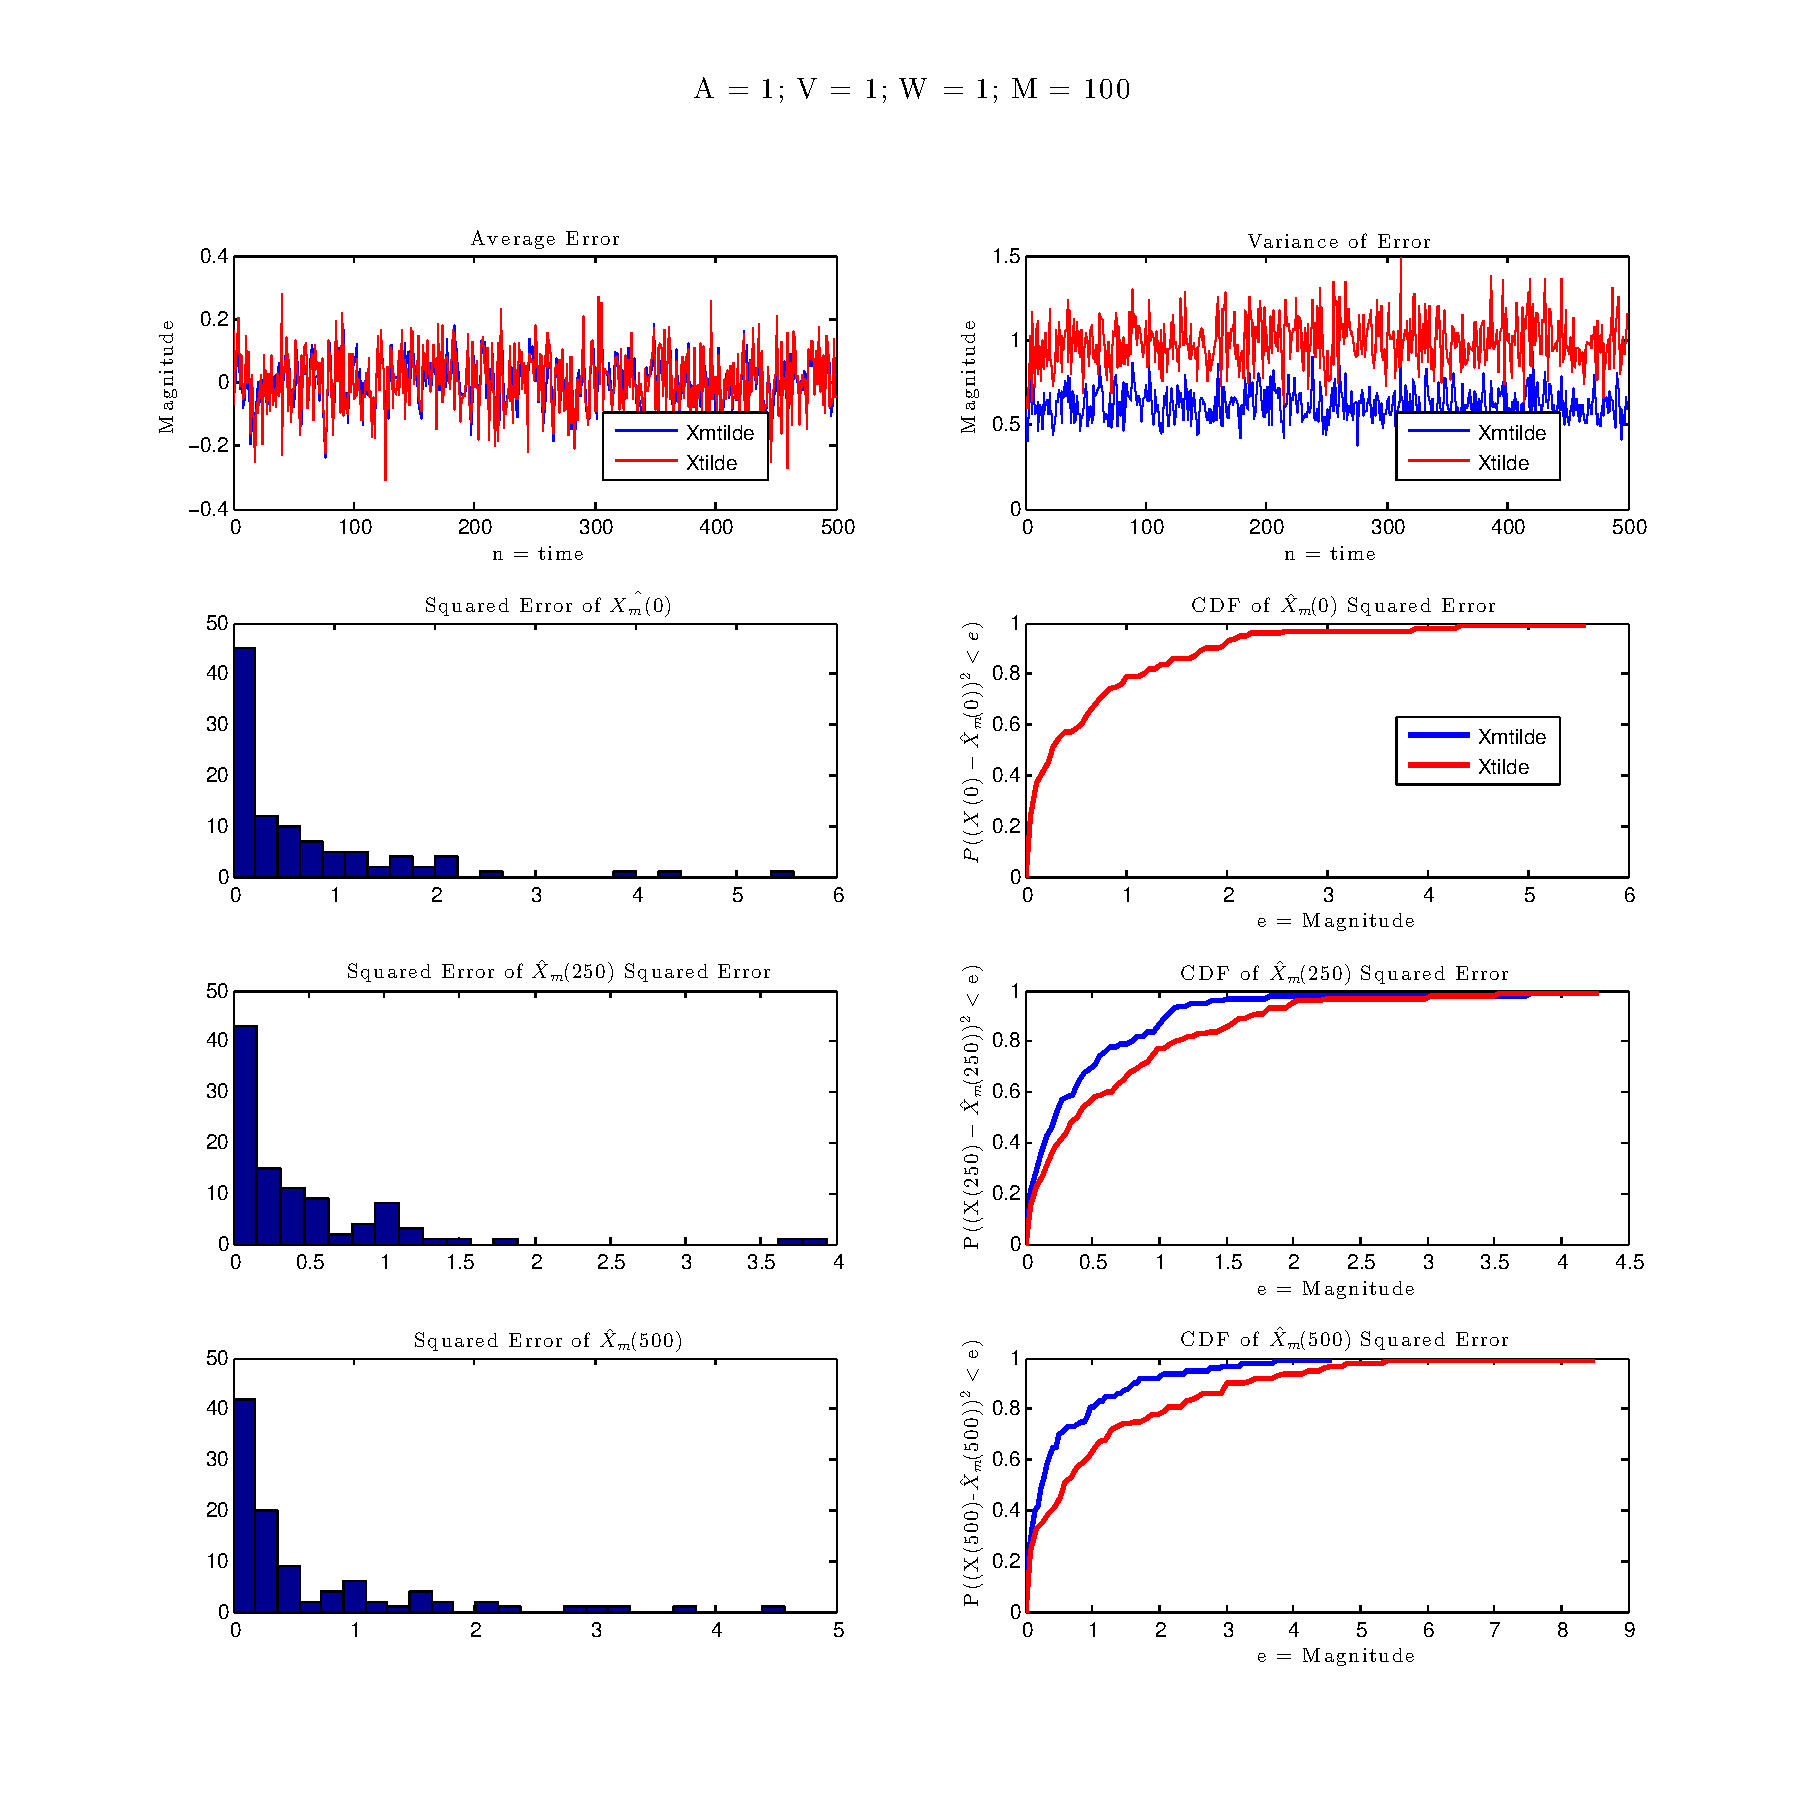
\includegraphics[width=\textwidth]{/Users/leahdickstein/Dropbox/R.edu/Sahai/140626/fig1_m100}
\end{minipage}
\begin{minipage}[c]{0.5\textwidth}
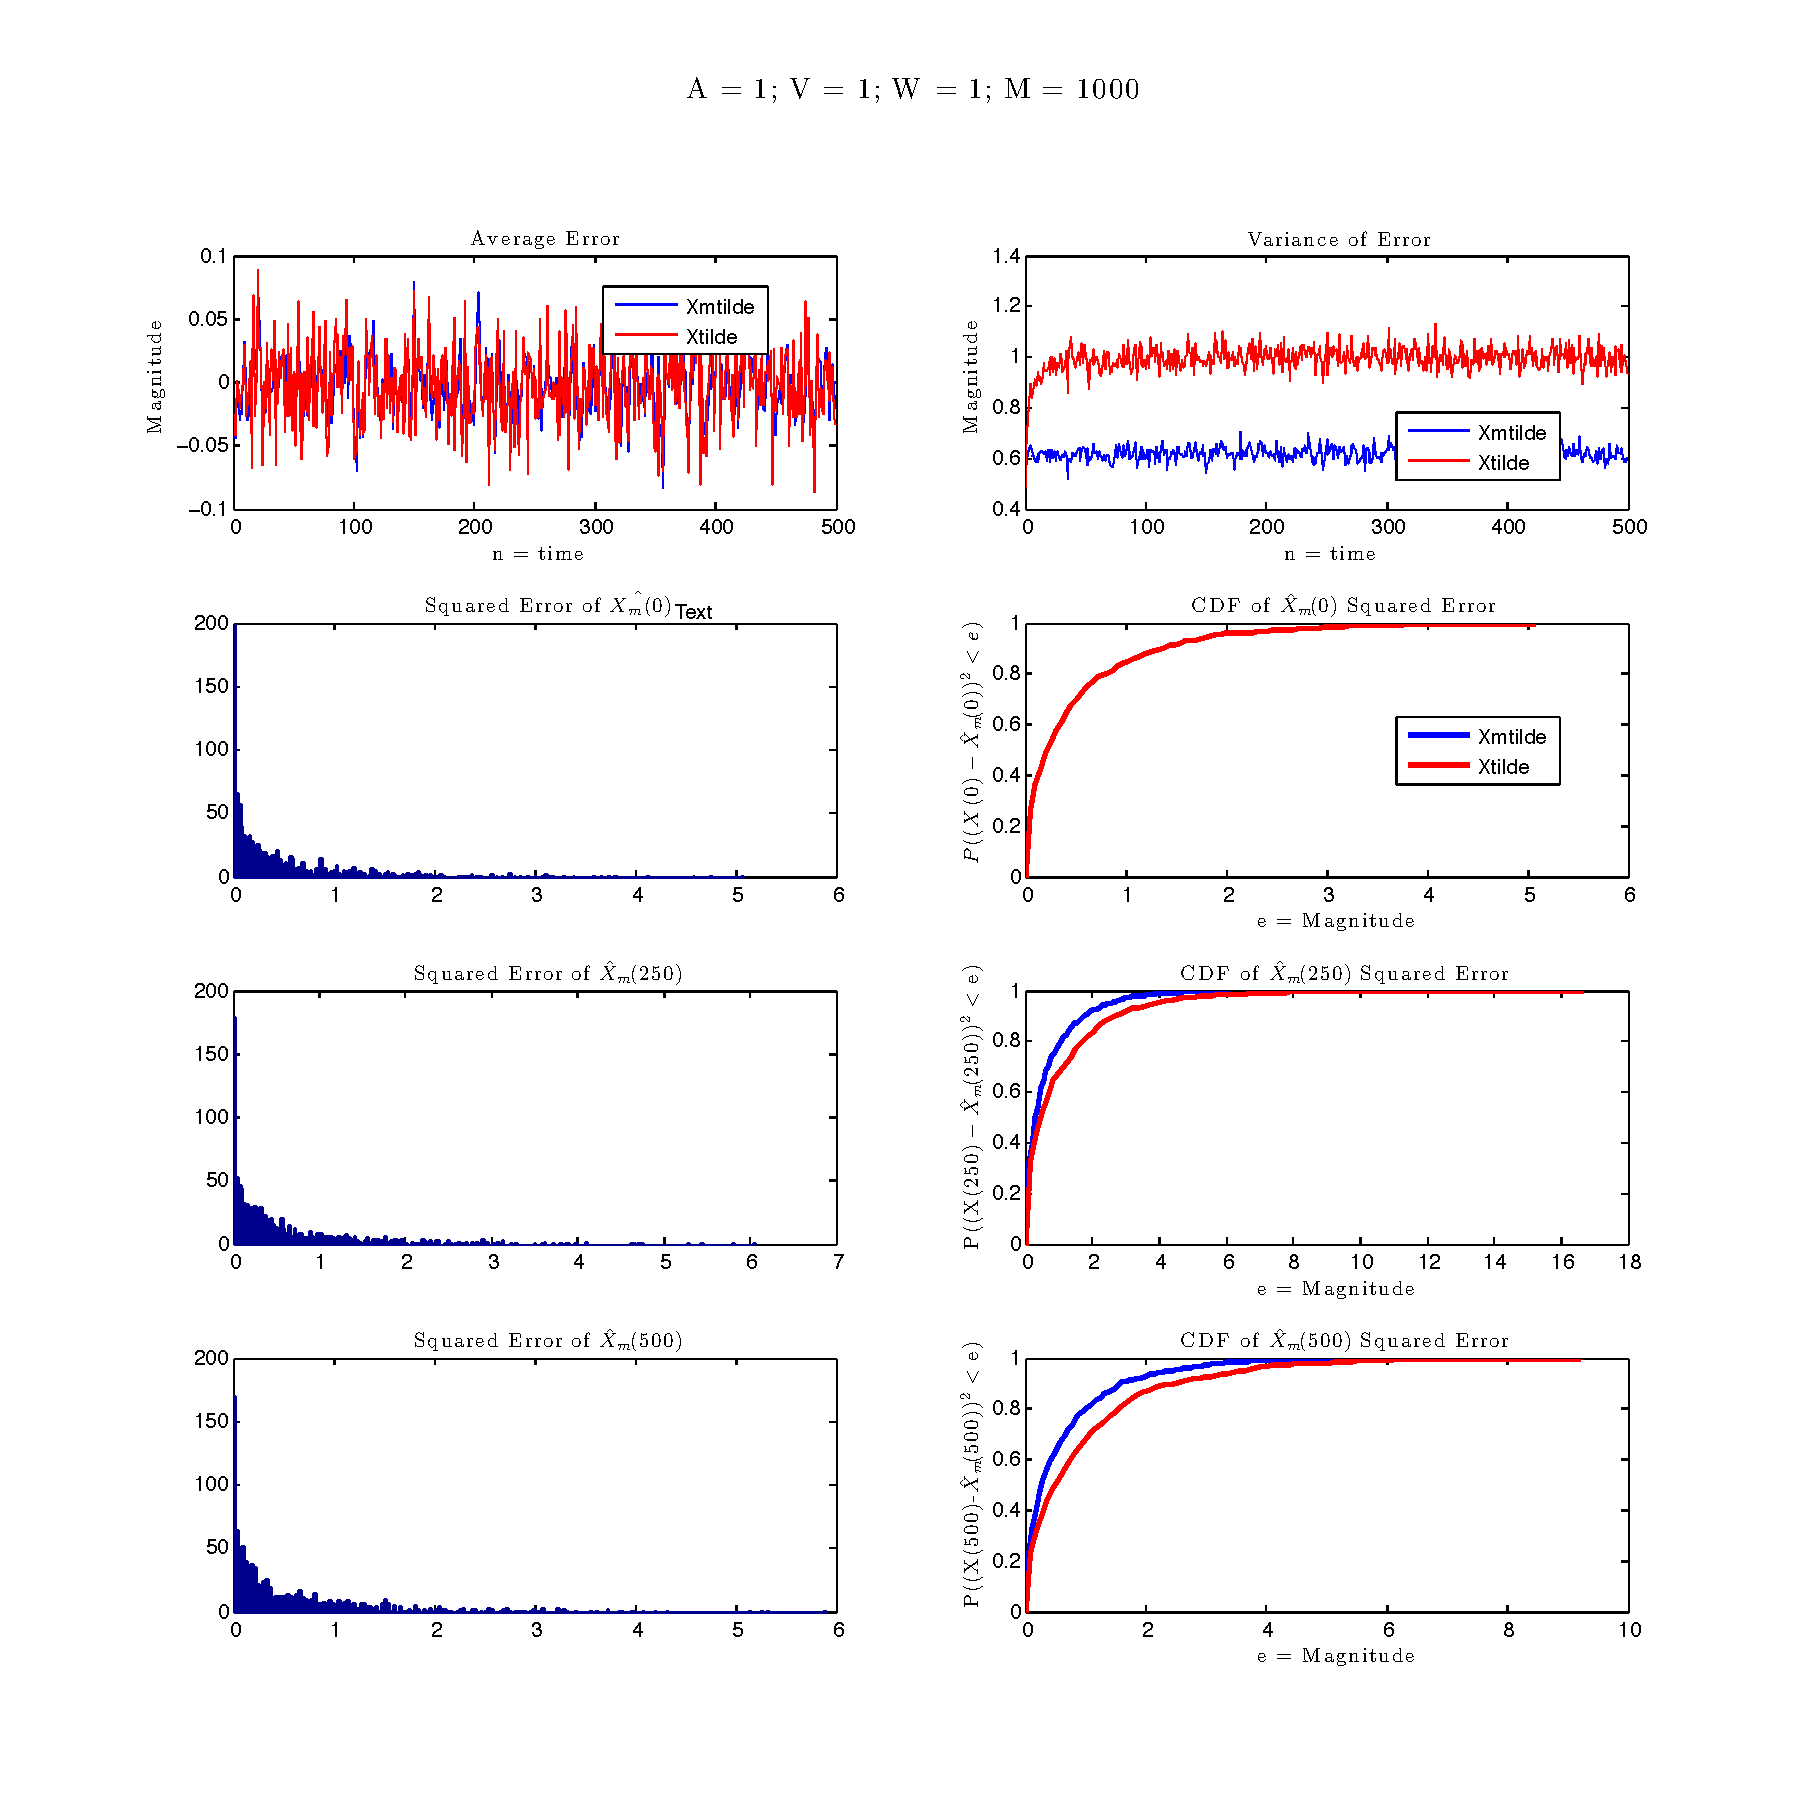
\includegraphics[width=\textwidth]{/Users/leahdickstein/Dropbox/R.edu/Sahai/140626/fig1_m1000}
\end{minipage}
These two figures represent a Kalman Filter with Additive Noise estimating a system with only additive noise. Xtilde represents a memoryless estimate, while Xmtilde represents the Kalman Filter's estimate.
\begin{itemize}
\item The estimation error variance is bounded
\item The Kalman Filter performs better than the optimal memoryless estimator; over many trials it's clearer the error variance is lower
\item If $0 < A < 1$, $Xmtilde \rightarrow Xtilde$. We showed earlier that the Kalman Filter is only intended for an estimation system, not a control system, and as the value of the state converges to 0 the estimation system behaves like the control problem. Since the value of the state is so close to 0 at each timestep, memory provides no additional benefit/utility to estimation.
\item The CDF of estimation error is affected by C, V, and W
\end{itemize}
\textbf{Note}: CDF of $\hat{X}_m(n)$ Squared Error means the plots are of the estimation error.

\subsection{Kalman Filter Ignoring Multiplicative Noise}
\begin{minipage}[c]{0.5\textwidth}
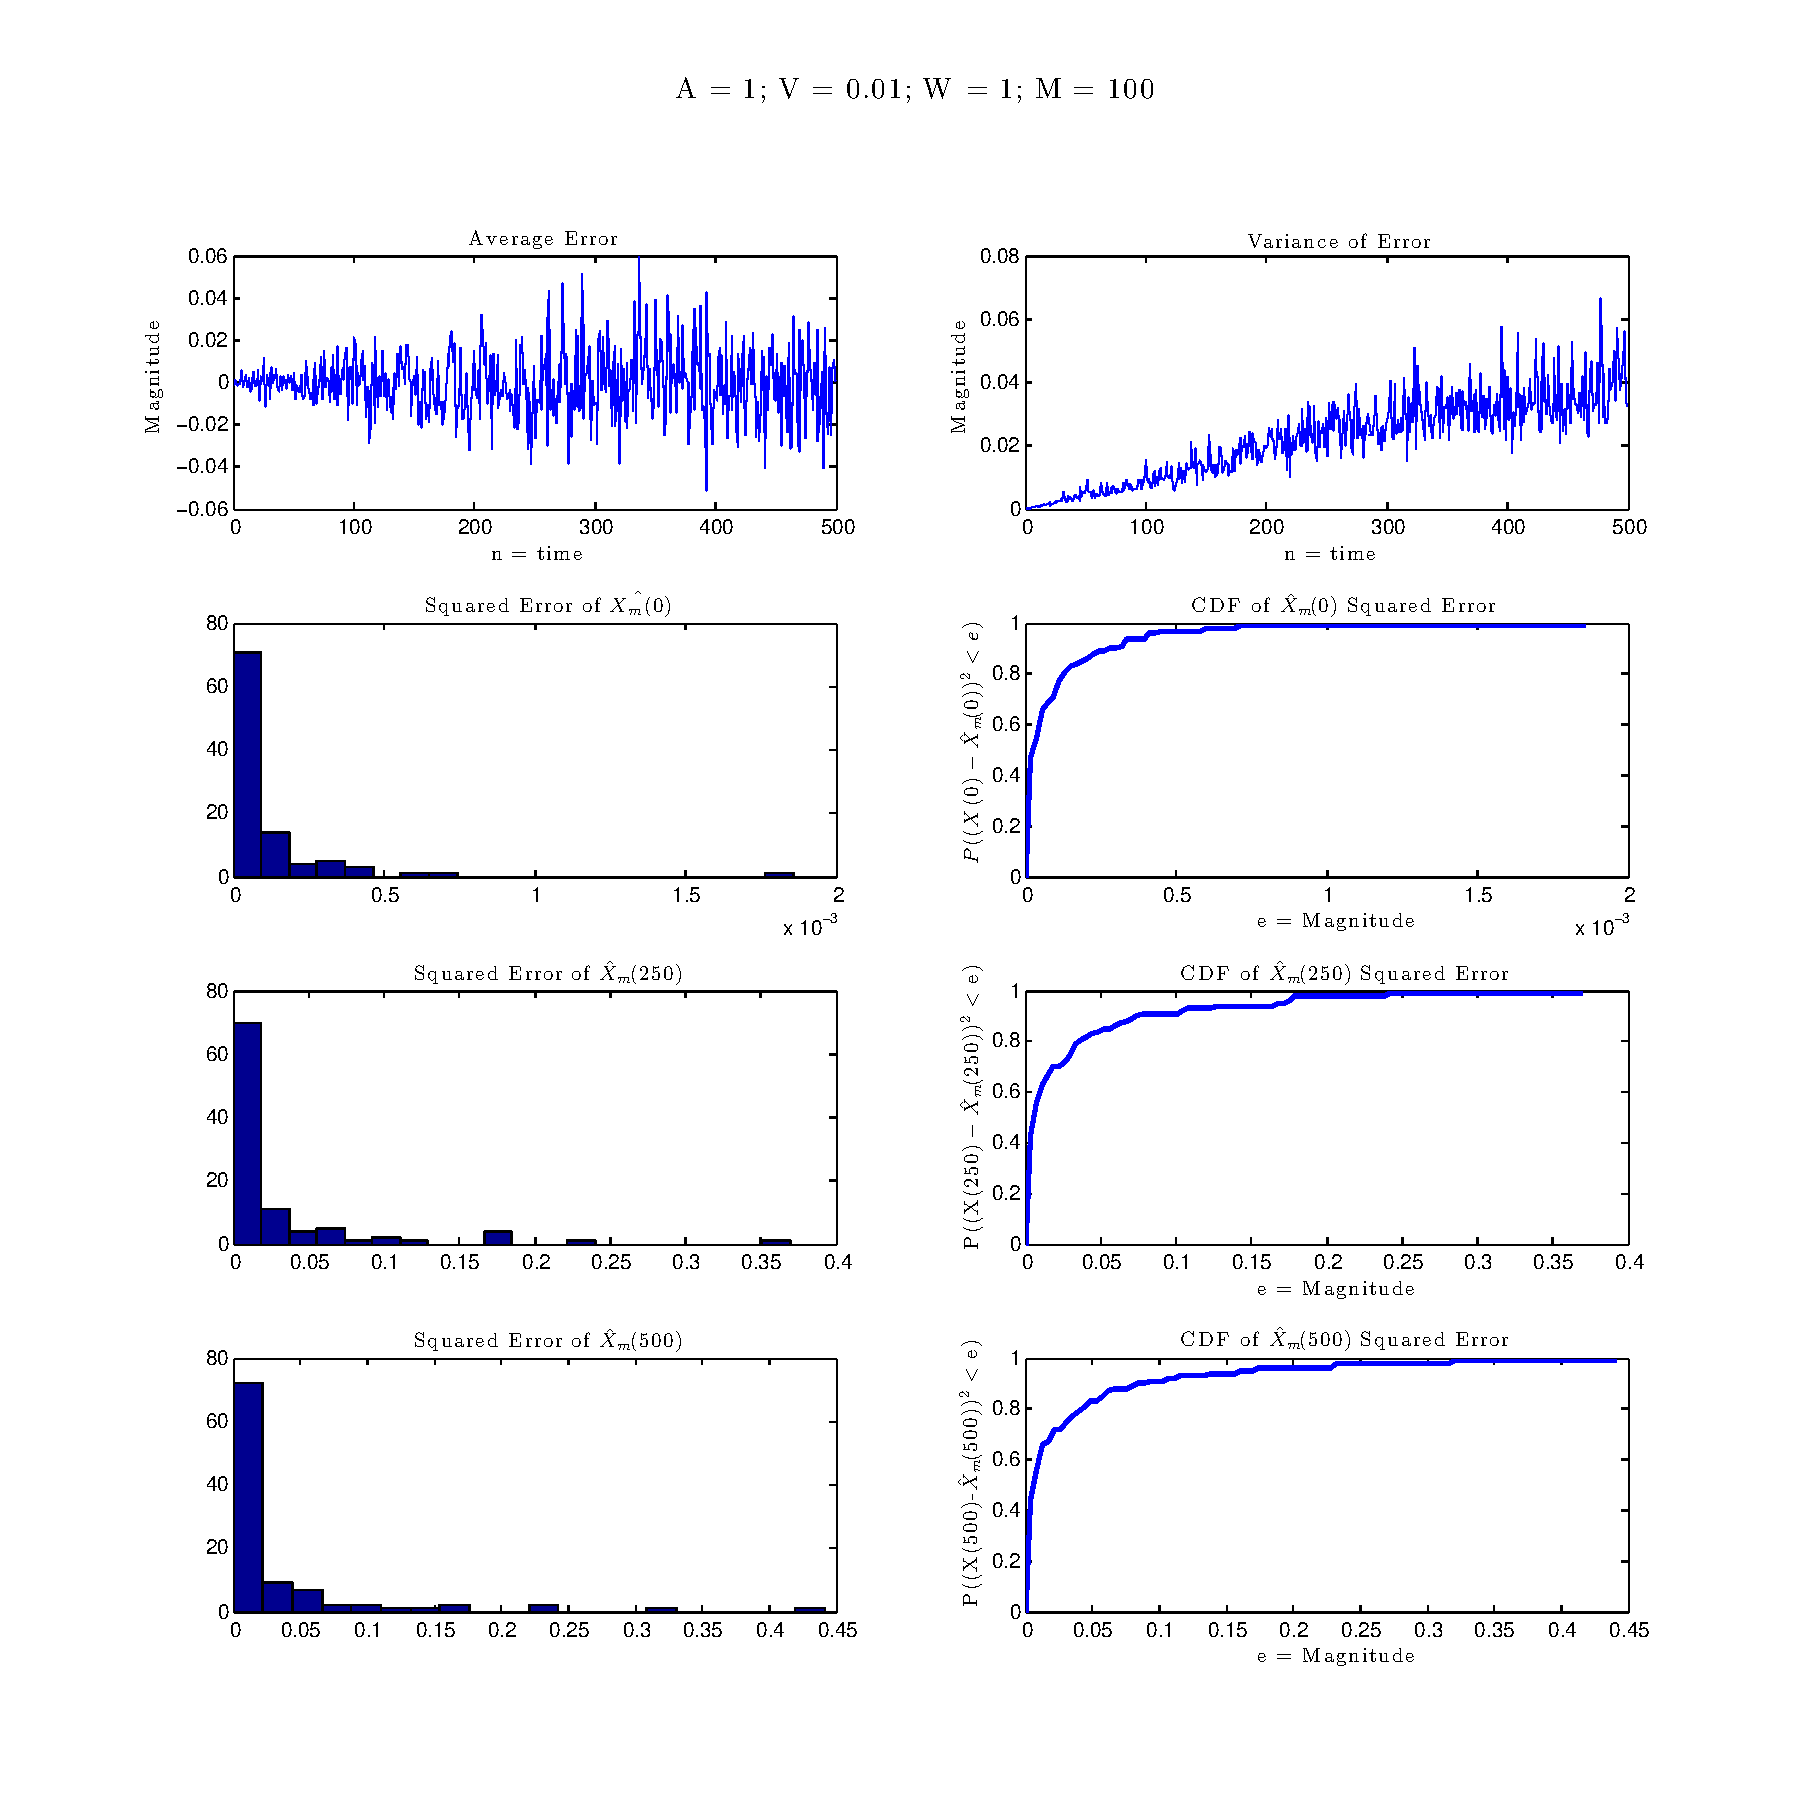
\includegraphics[width=\textwidth]{/Users/leahdickstein/Dropbox/R.edu/Sahai/140626/fig2_v001_m100}
\end{minipage}
\begin{minipage}[c]{0.5\textwidth}
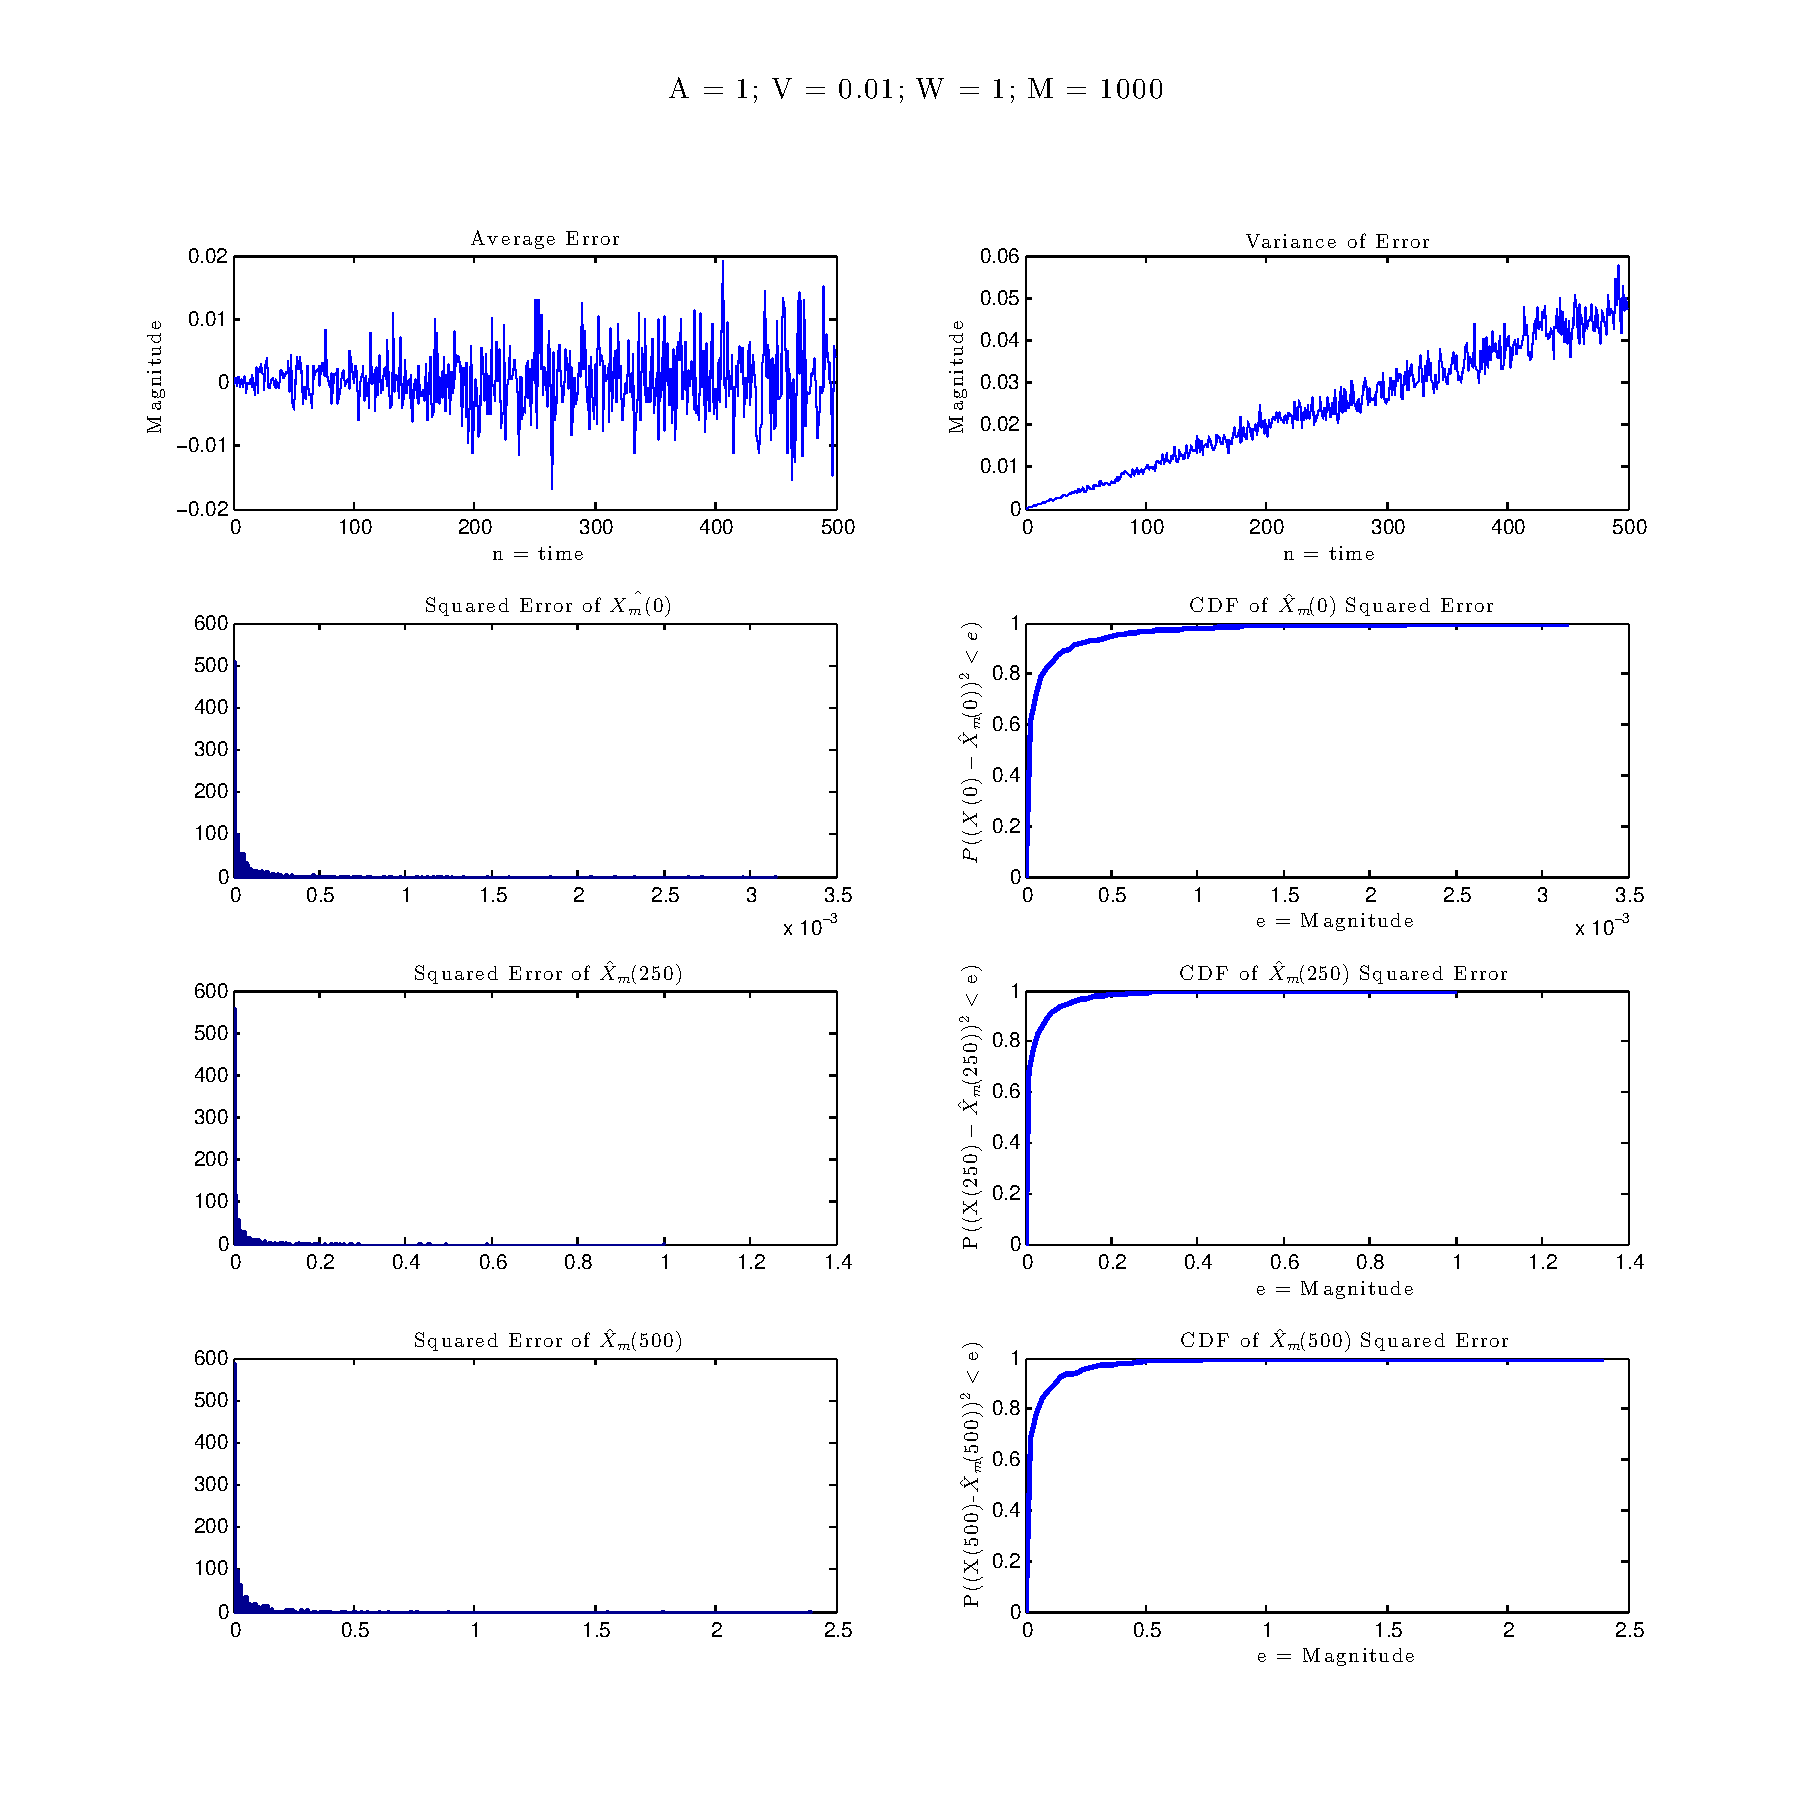
\includegraphics[width=\textwidth]{/Users/leahdickstein/Dropbox/R.edu/Sahai/140626/fig2_v001_m1000}
\end{minipage}

\begin{minipage}[c]{0.5\textwidth}
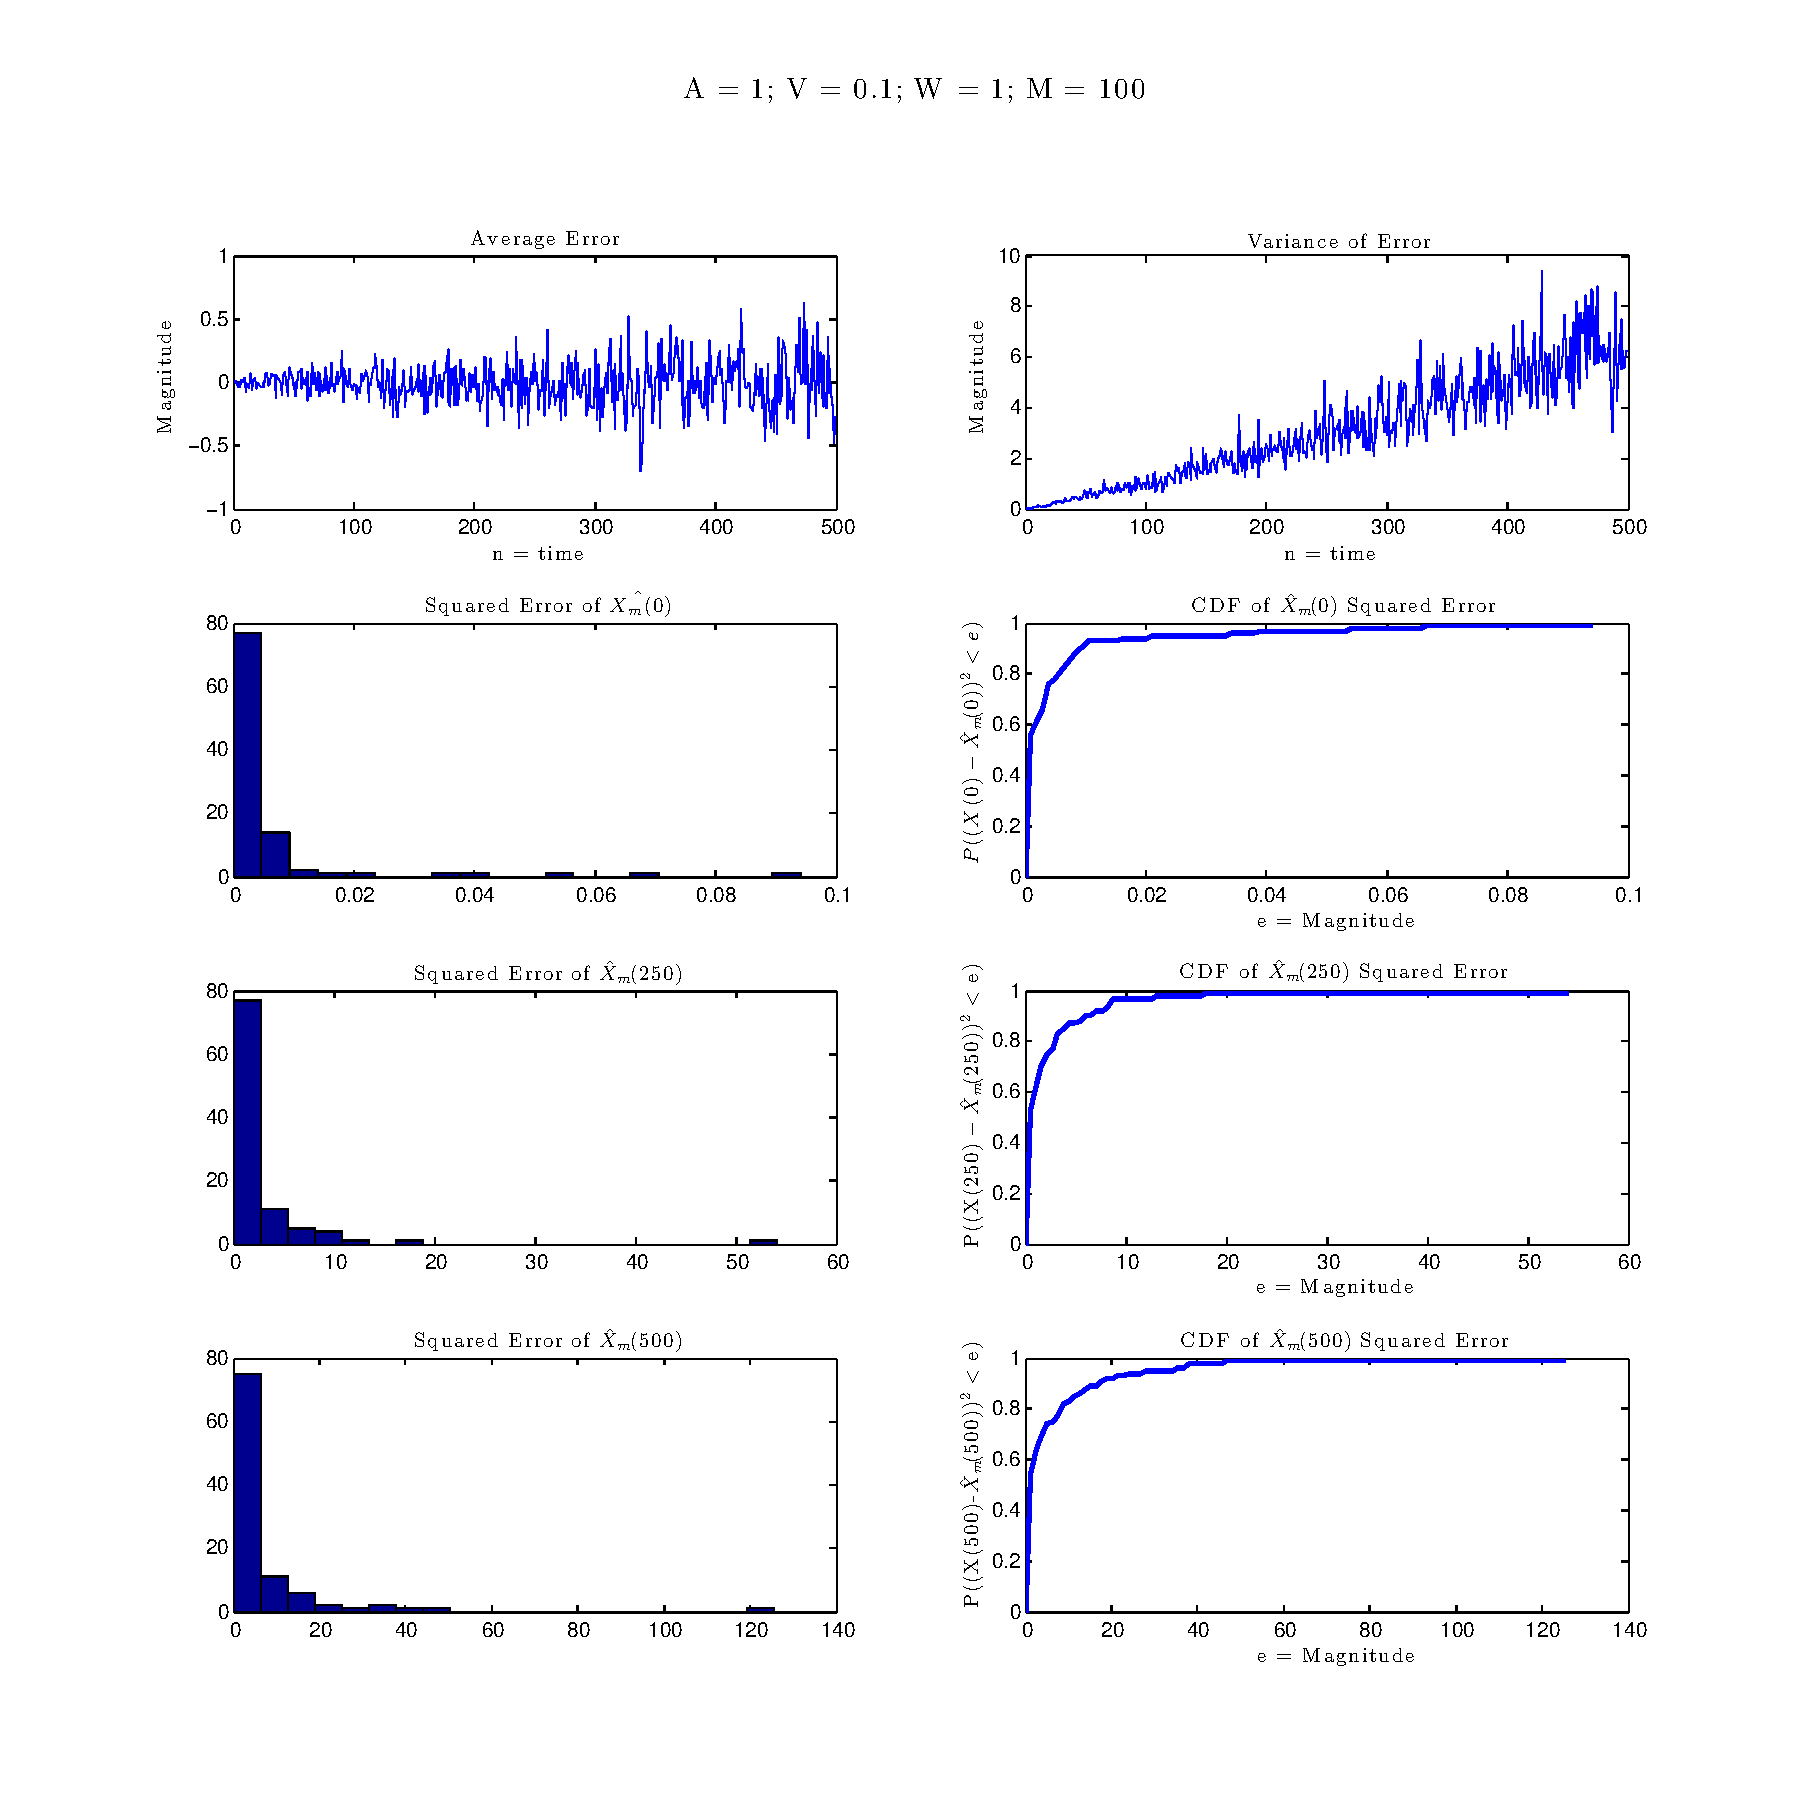
\includegraphics[width=\textwidth]{/Users/leahdickstein/Dropbox/R.edu/Sahai/140626/fig2_v01_m100}
\end{minipage}
\begin{minipage}[c]{0.5\textwidth}
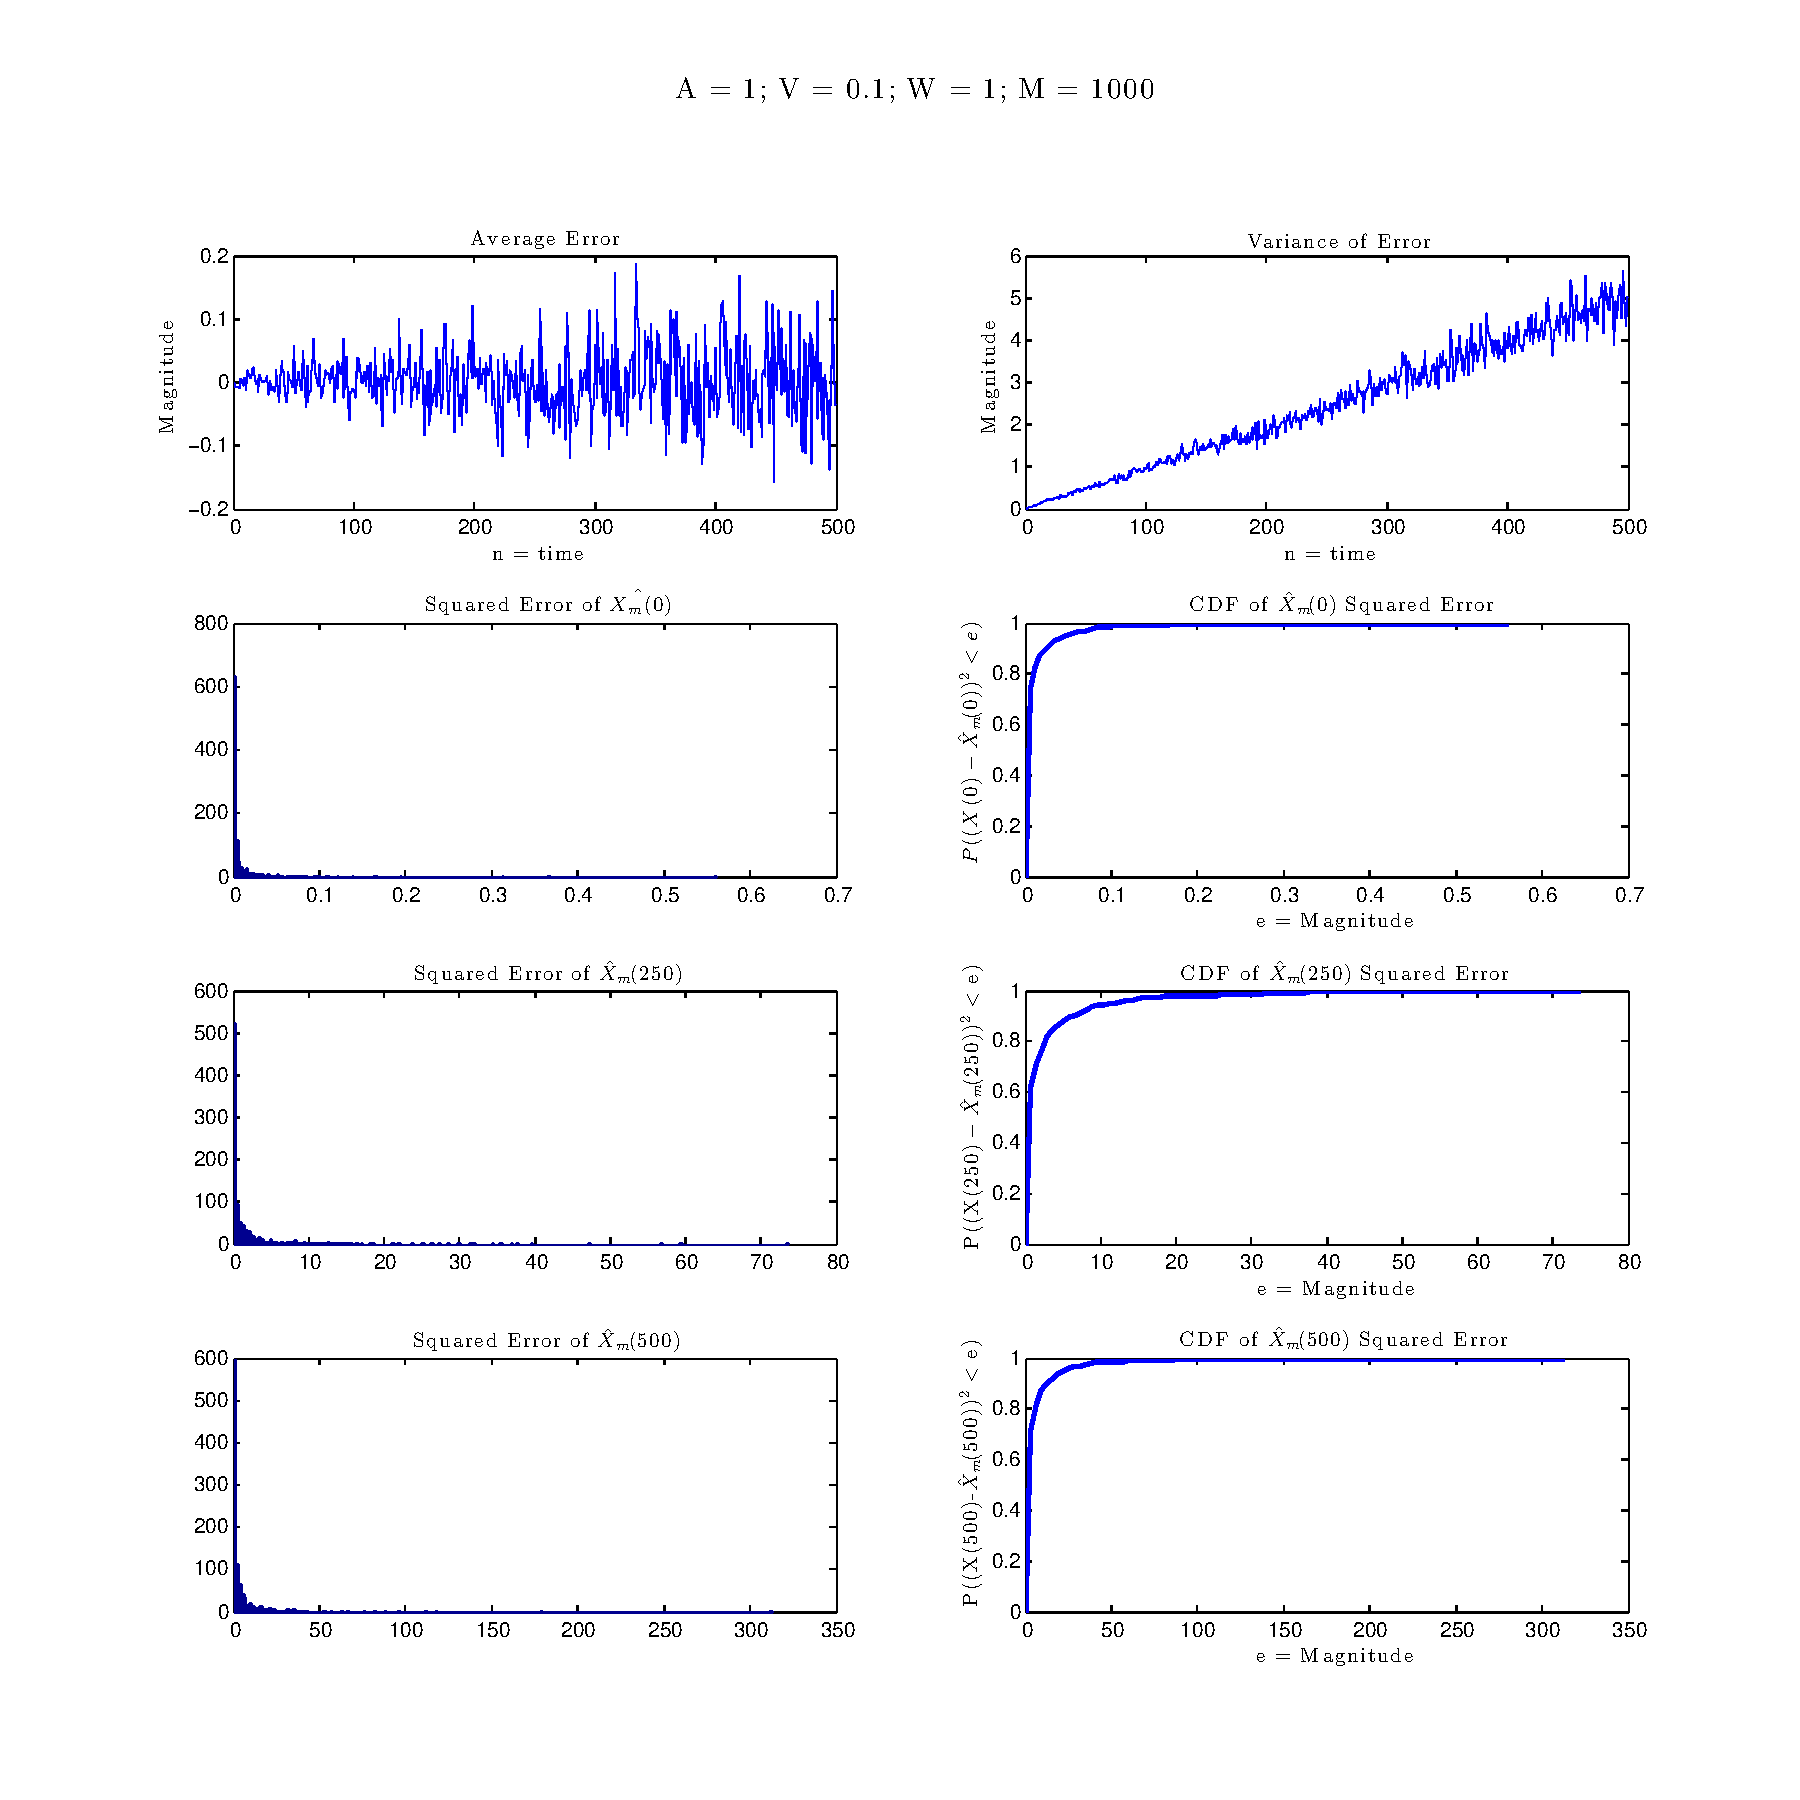
\includegraphics[width=\textwidth]{/Users/leahdickstein/Dropbox/R.edu/Sahai/140626/fig2_v01_m1000}
\end{minipage}

\begin{minipage}[c]{0.5\textwidth}
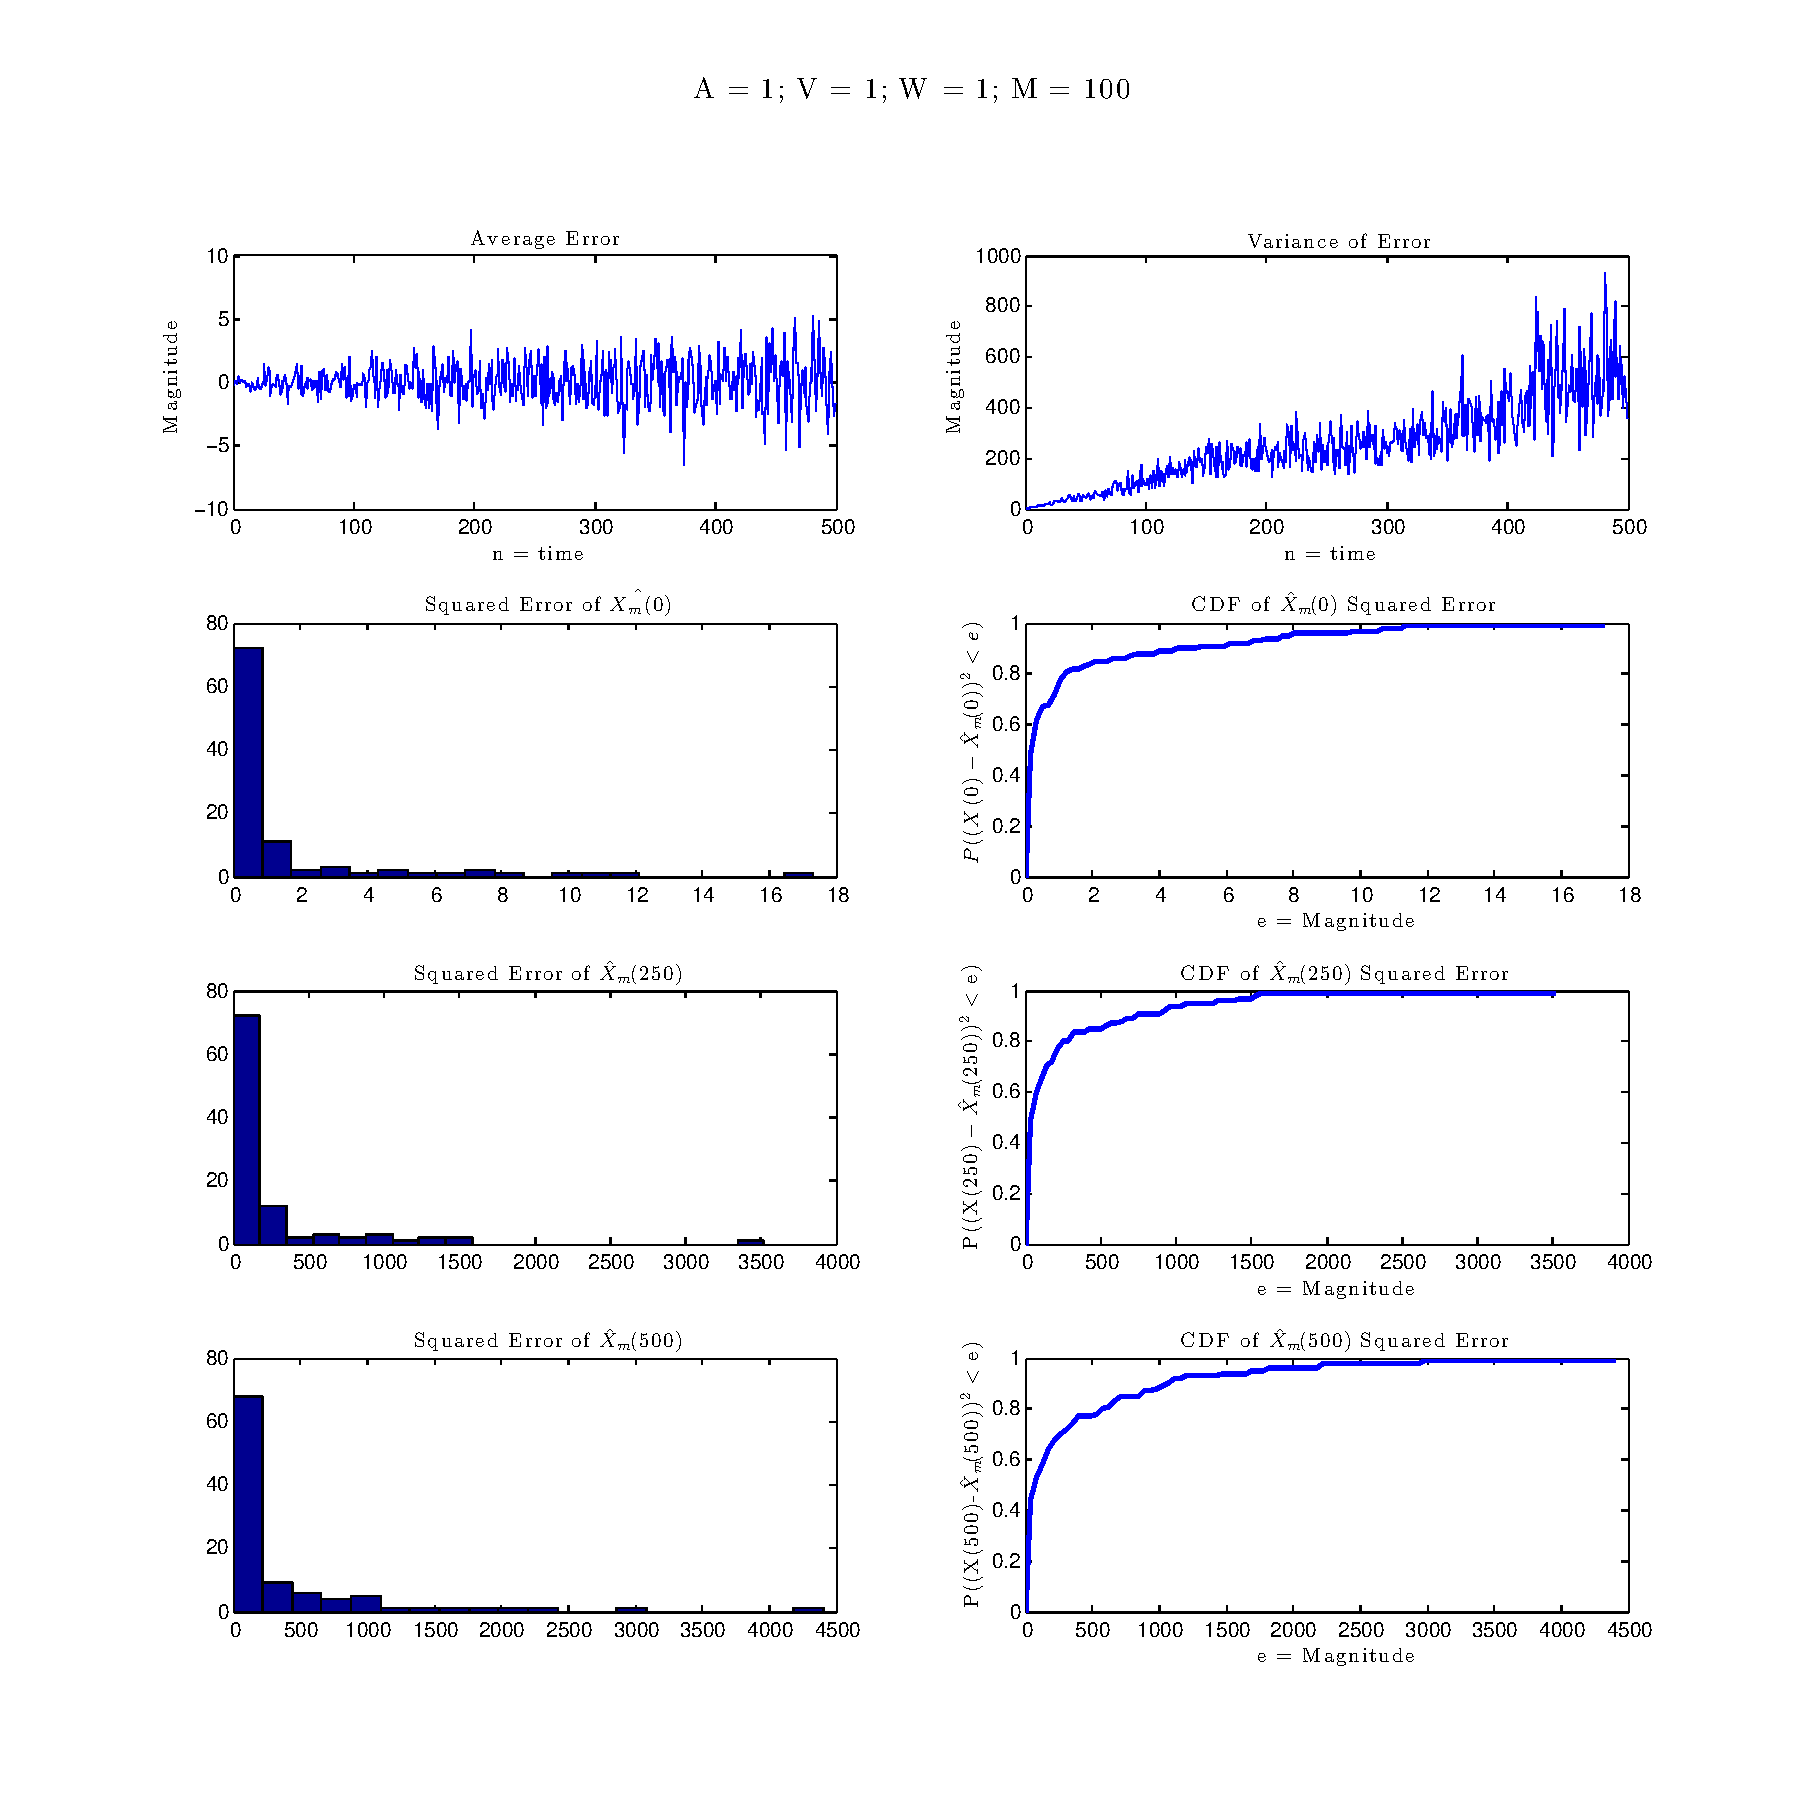
\includegraphics[width=\textwidth]{/Users/leahdickstein/Dropbox/R.edu/Sahai/140626/fig2_v1_m100}
\end{minipage}
\begin{minipage}[c]{0.5\textwidth}
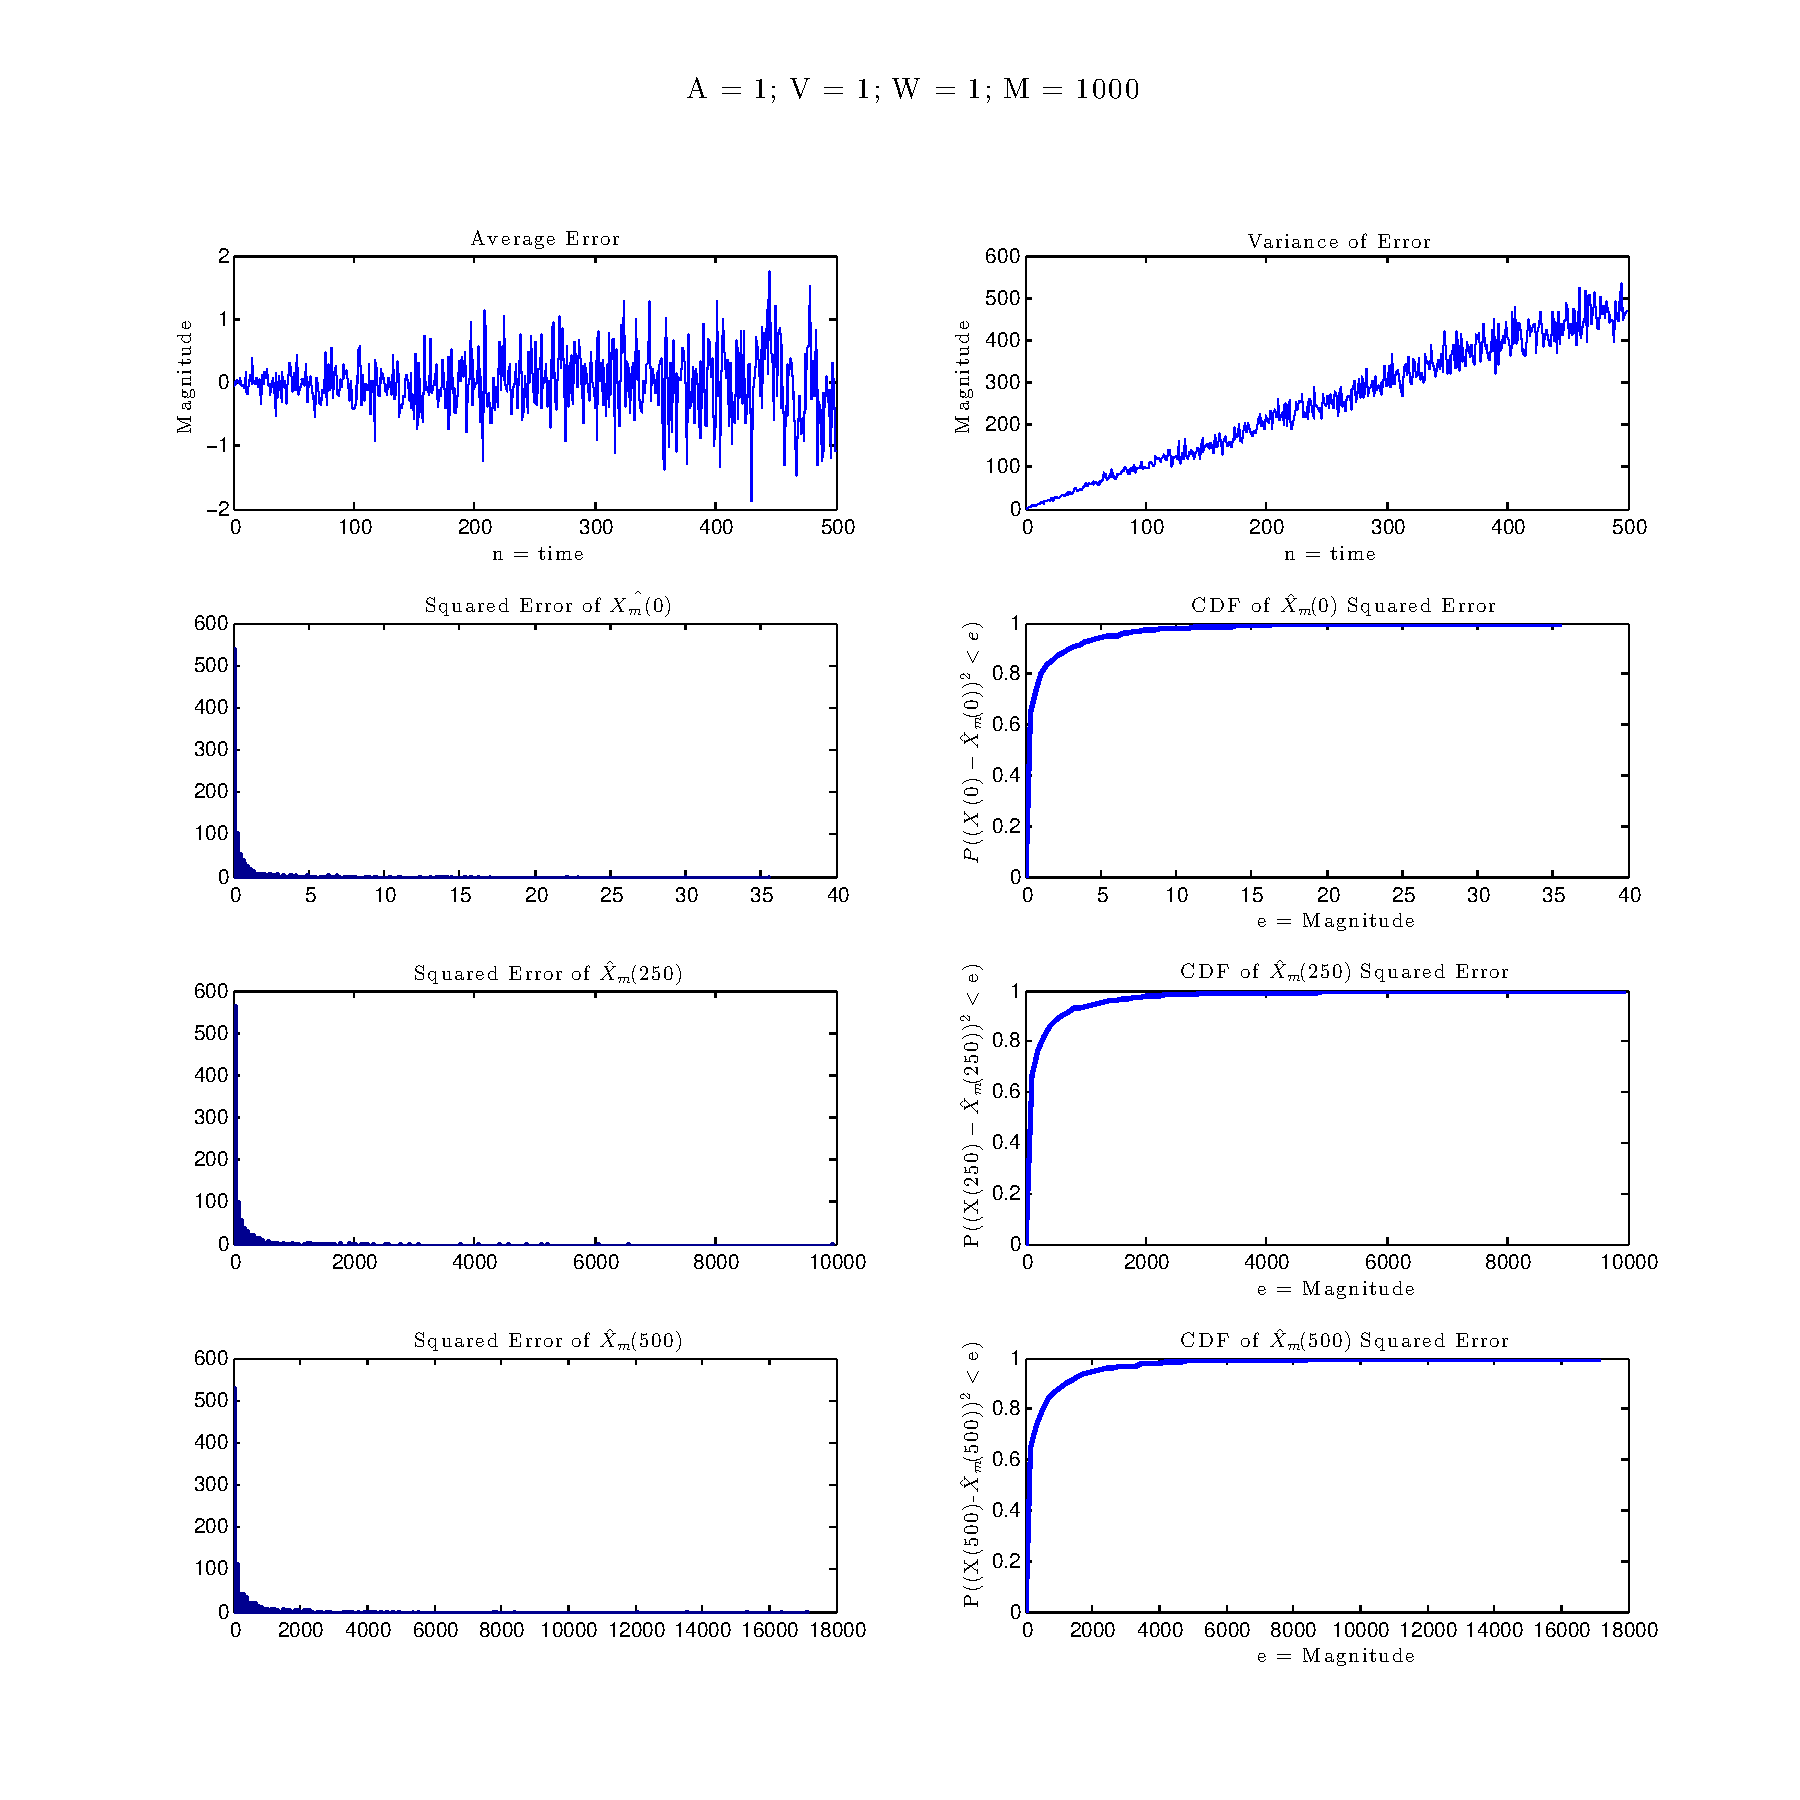
\includegraphics[width=\textwidth]{/Users/leahdickstein/Dropbox/R.edu/Sahai/140626/fig2_v1_m1000}
\end{minipage}

\begin{minipage}[c]{0.5\textwidth}
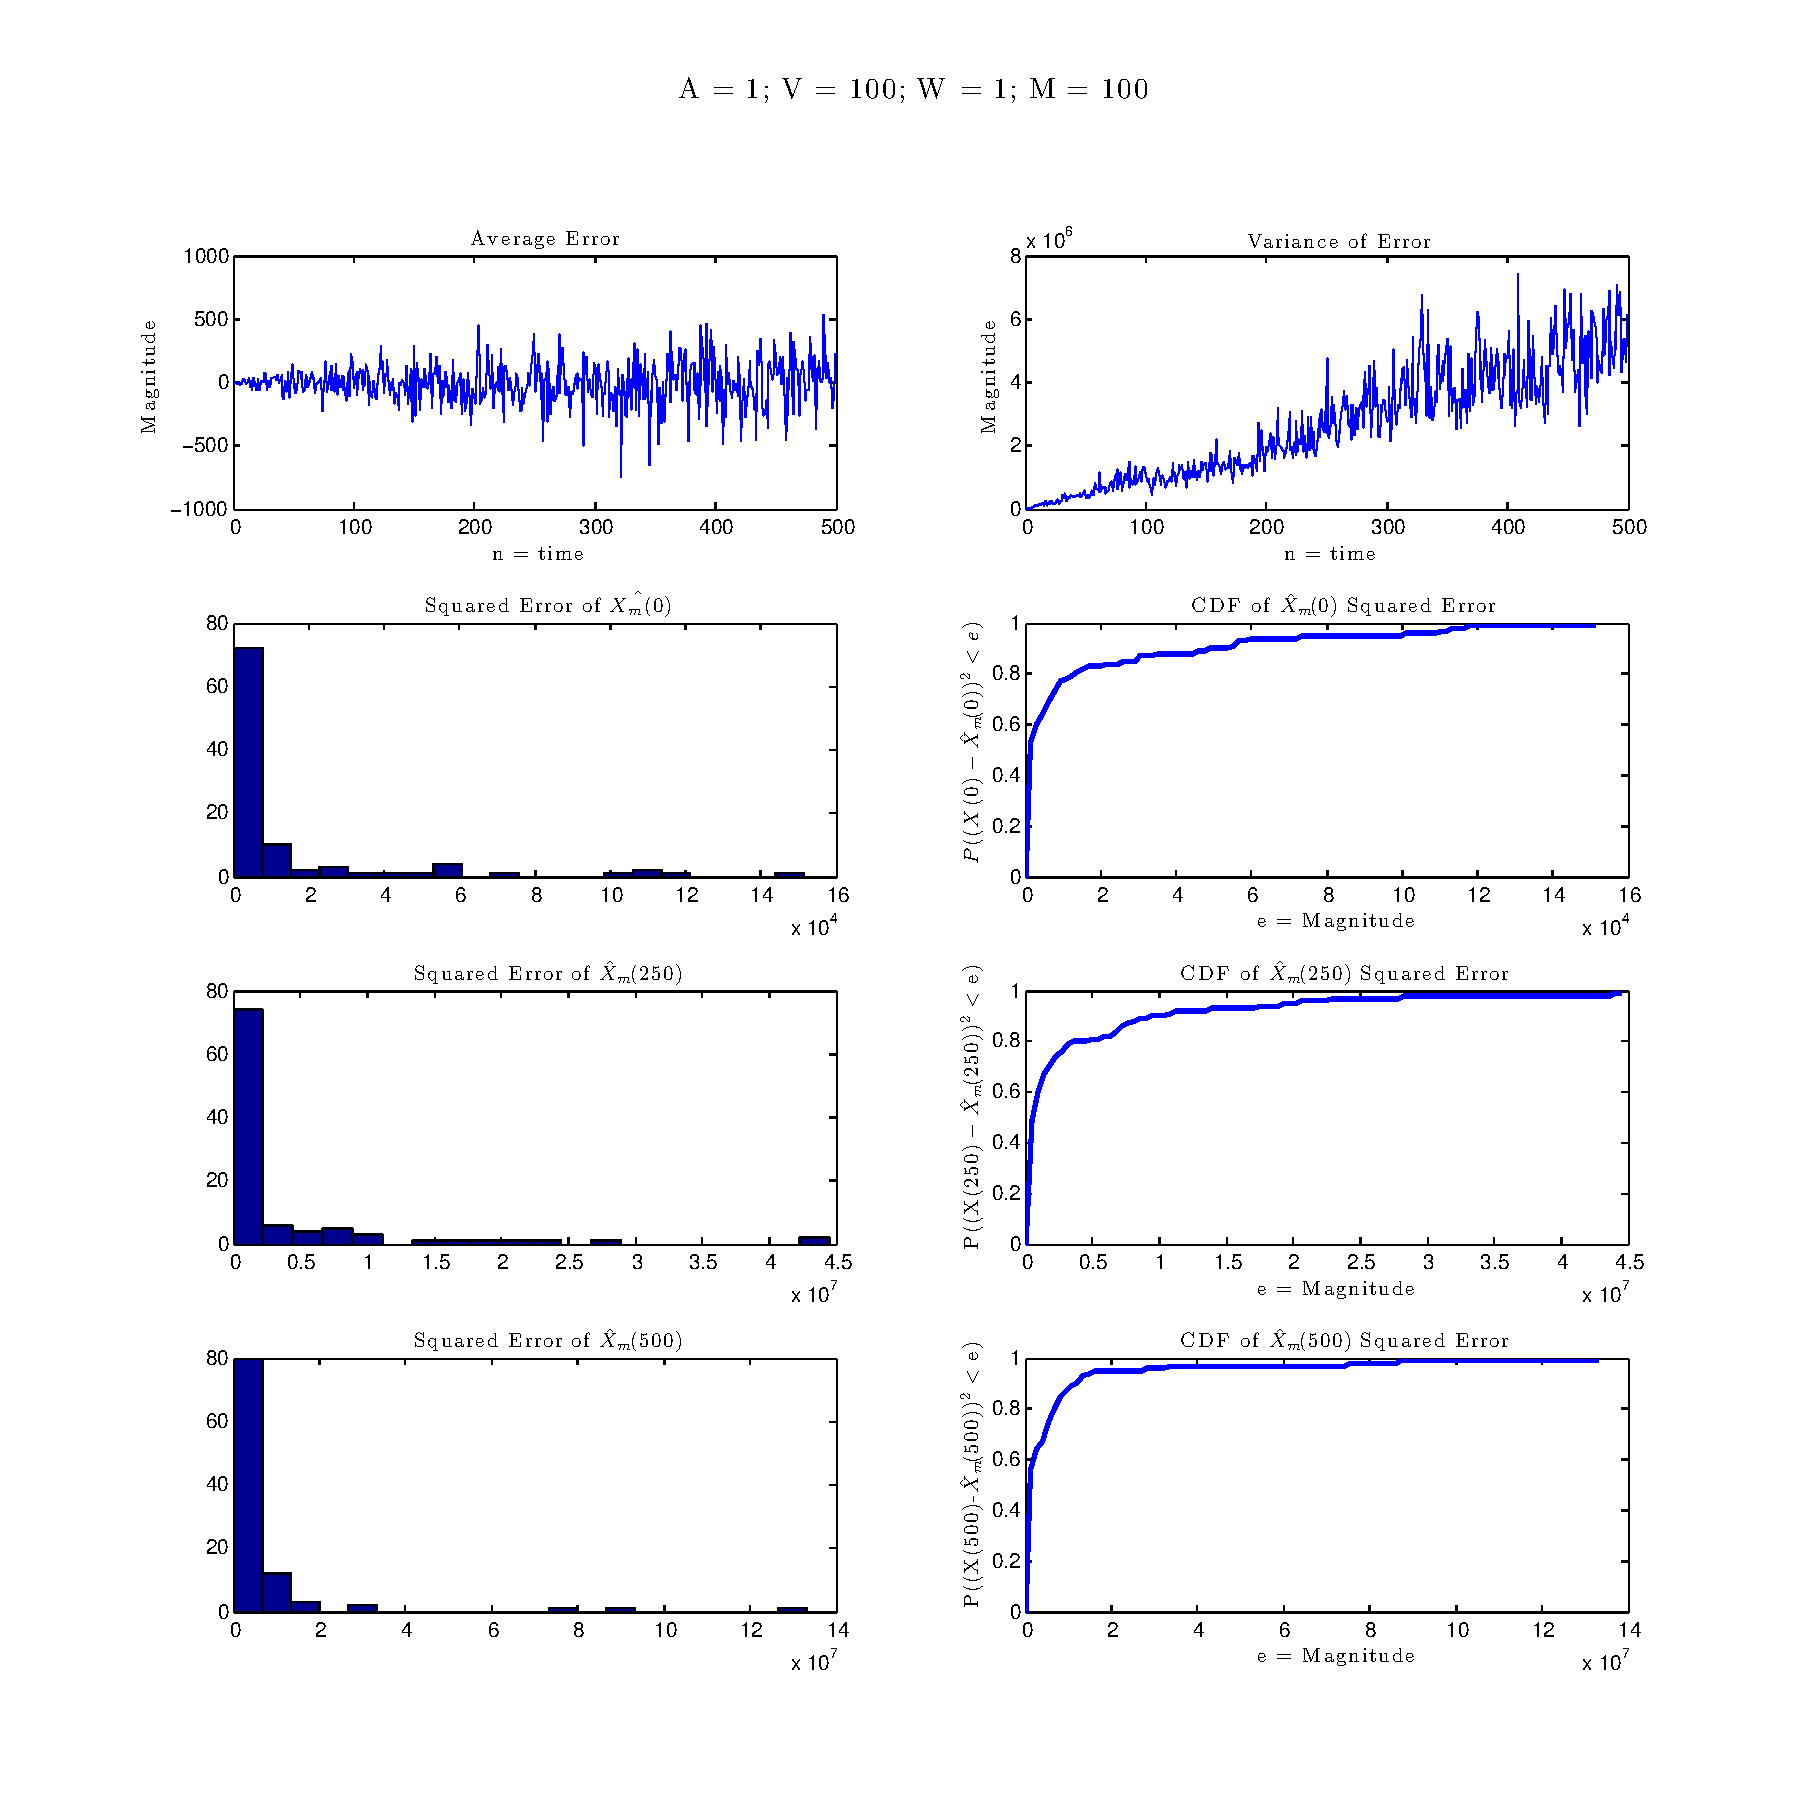
\includegraphics[width=\textwidth]{/Users/leahdickstein/Dropbox/R.edu/Sahai/140626/fig2_v100_m100}
\end{minipage}
\begin{minipage}[c]{0.5\textwidth}
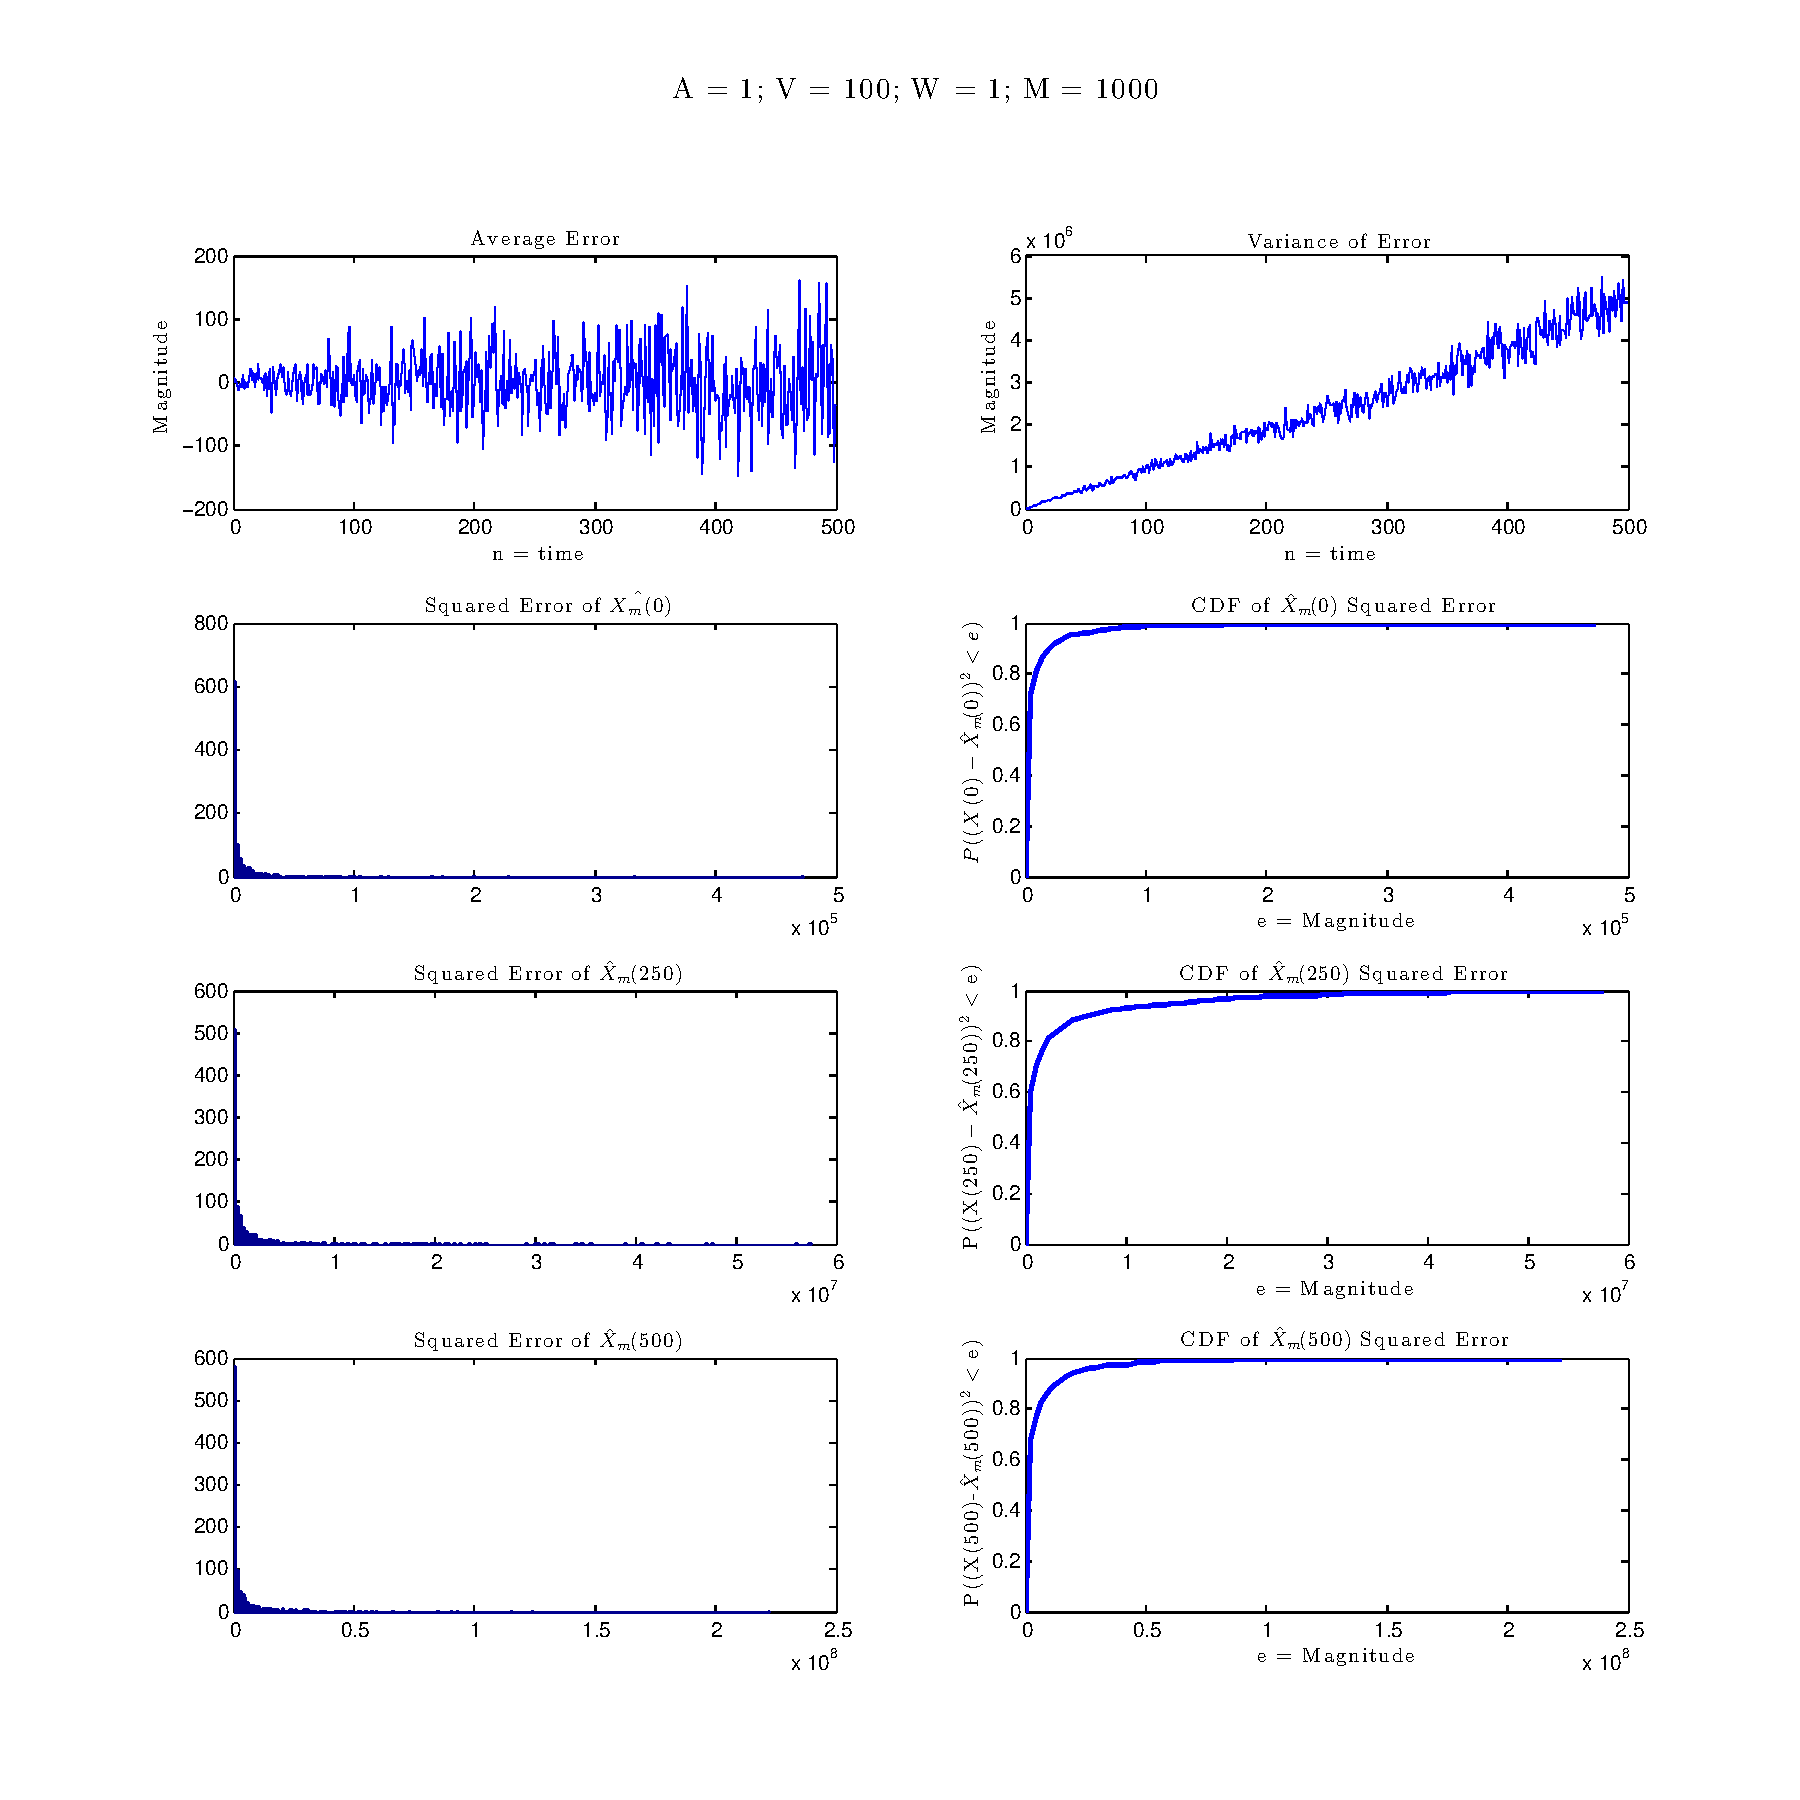
\includegraphics[width=\textwidth]{/Users/leahdickstein/Dropbox/R.edu/Sahai/140626/fig2_v100_m1000}
\end{minipage}

These figures represent a Kalman Filter for Additive Noise with a system that has state multiplicative noise and additive noise but no observation noise. The estimation error variance steadily increases because the multiplicative noise causes the signal to increase, thus increasing the error from the multiplicative noise. In this setup, the multiplicative error was $(1+r(n)) = (1+normrnd(0,varv))$. The four figures represent ascending levels of V (or $\frac{1}{p}$), with the estimation error variance increasing as V increases.\\
\textbf{Note}: CDF of $\hat{X}_m(n)$ Squared Error means the plots are of the estimation error.

\subsection{Kalman Filter for Multiplicative Noise}
\begin{minipage}[c]{0.5\textwidth}
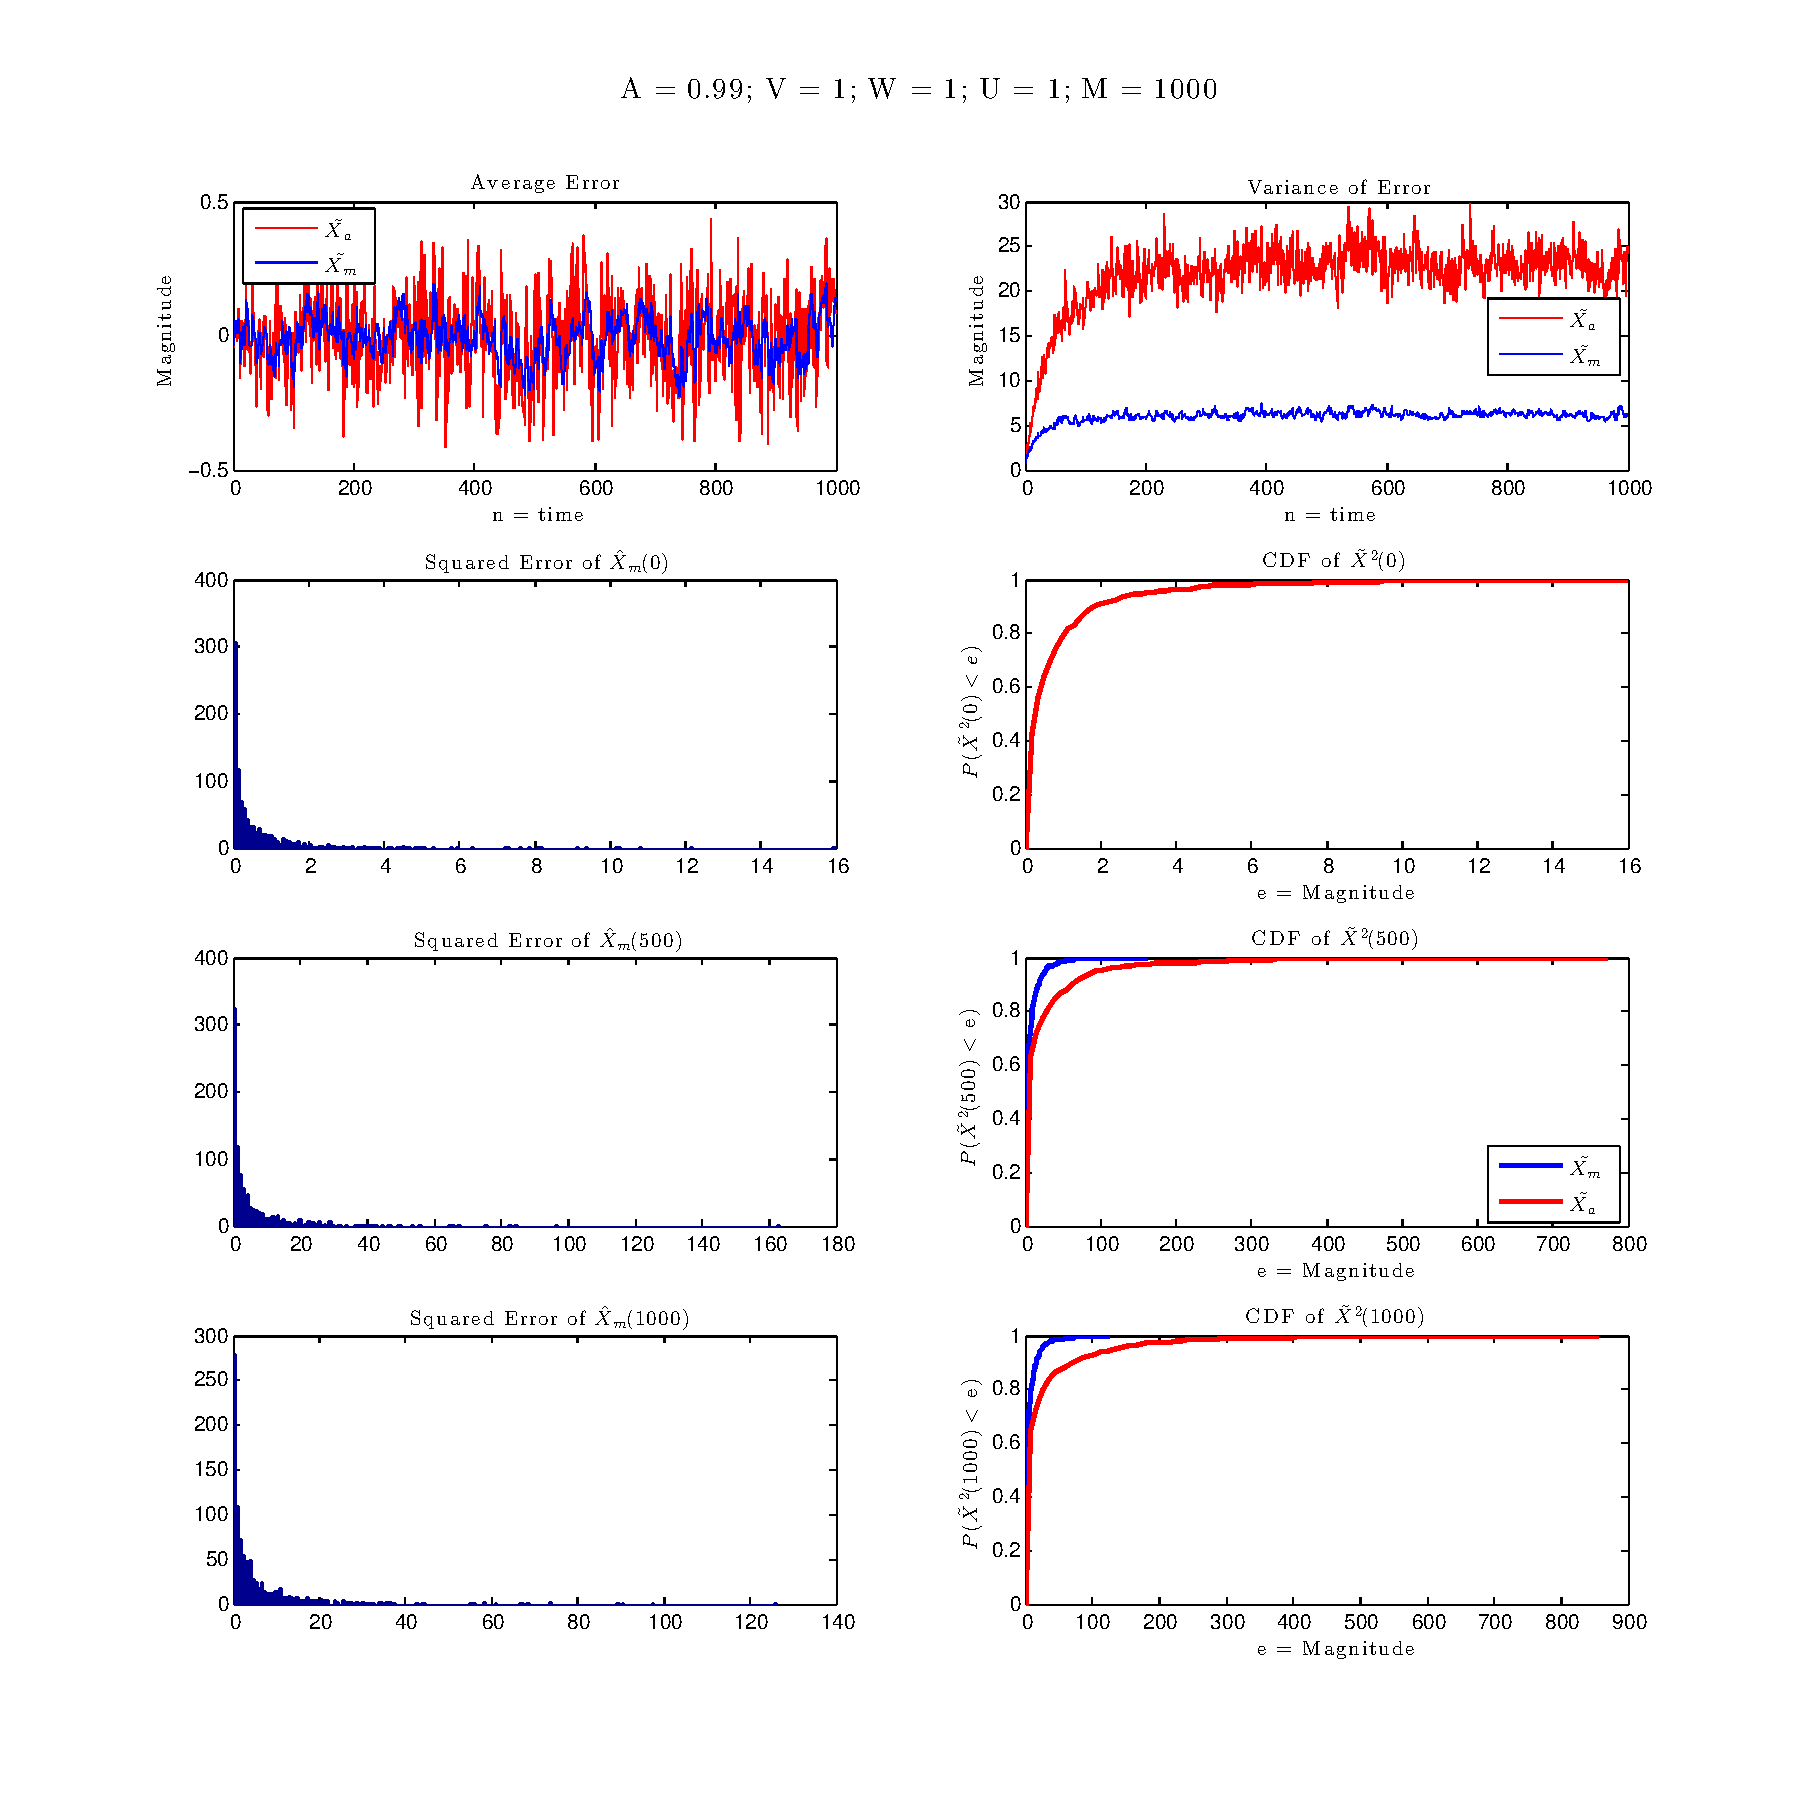
\includegraphics[width=\textwidth]{/Users/leahdickstein/Dropbox/R.edu/Sahai/140706/kfmul_a099_m1000}
\end{minipage}
\begin{minipage}[c]{0.5\textwidth}
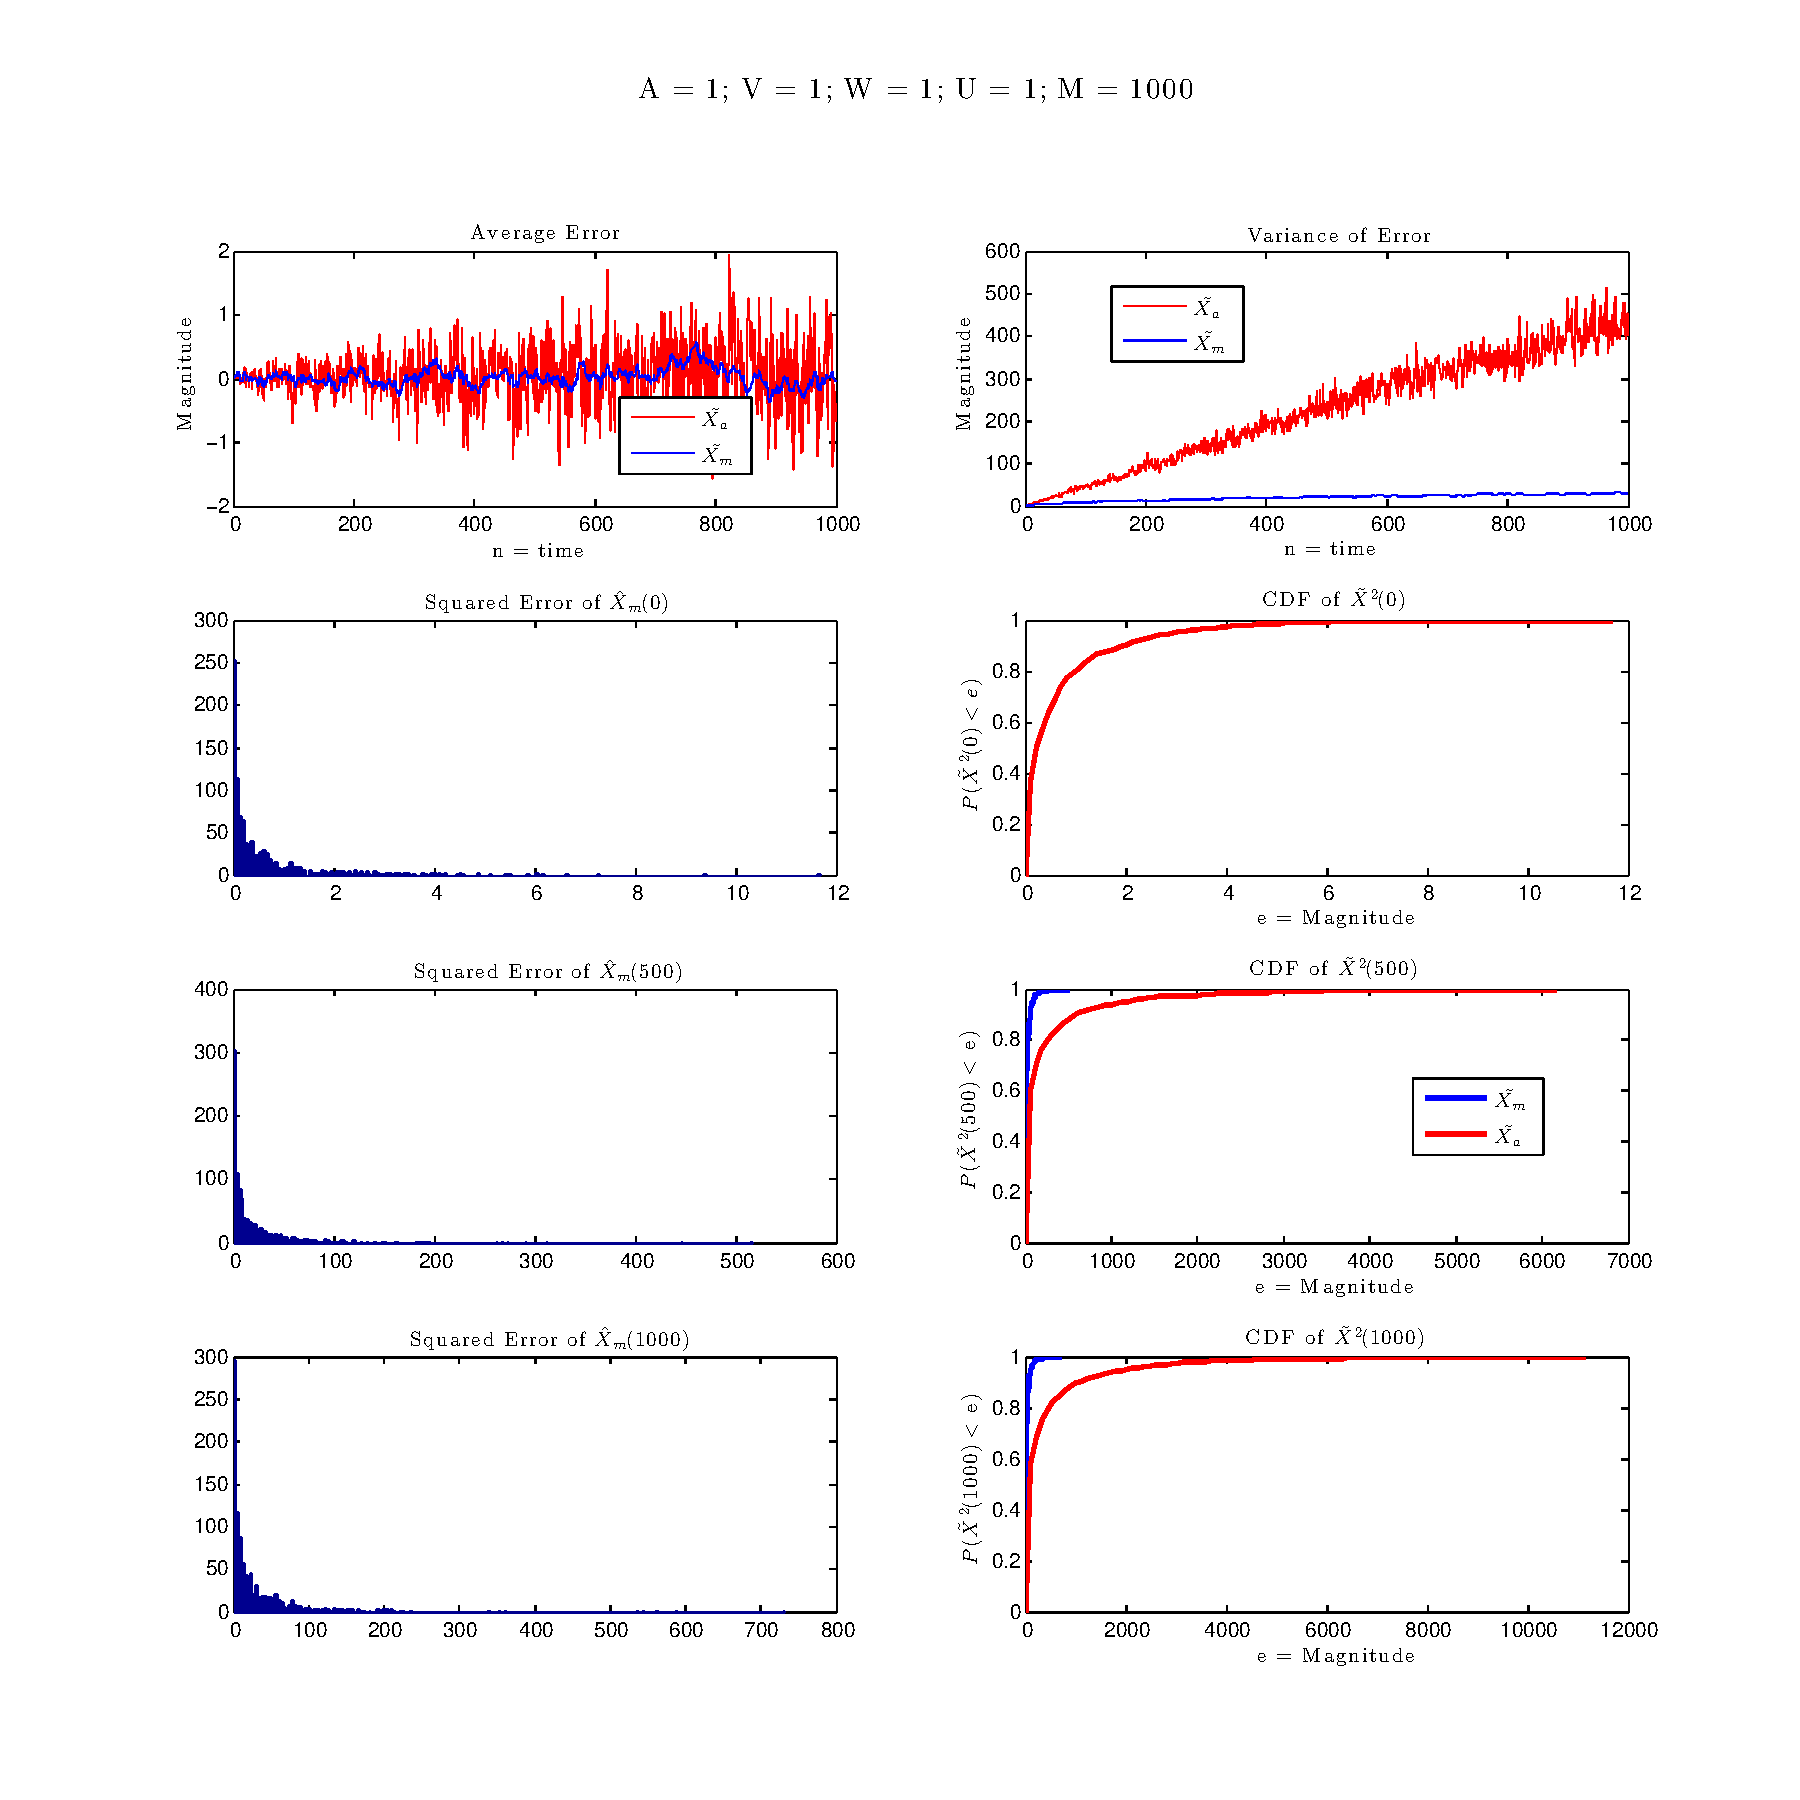
\includegraphics[width=\textwidth]{/Users/leahdickstein/Dropbox/R.edu/Sahai/140706/kfmul_a1_m1000}
\end{minipage}

\begin{minipage}[c]{0.5\textwidth}
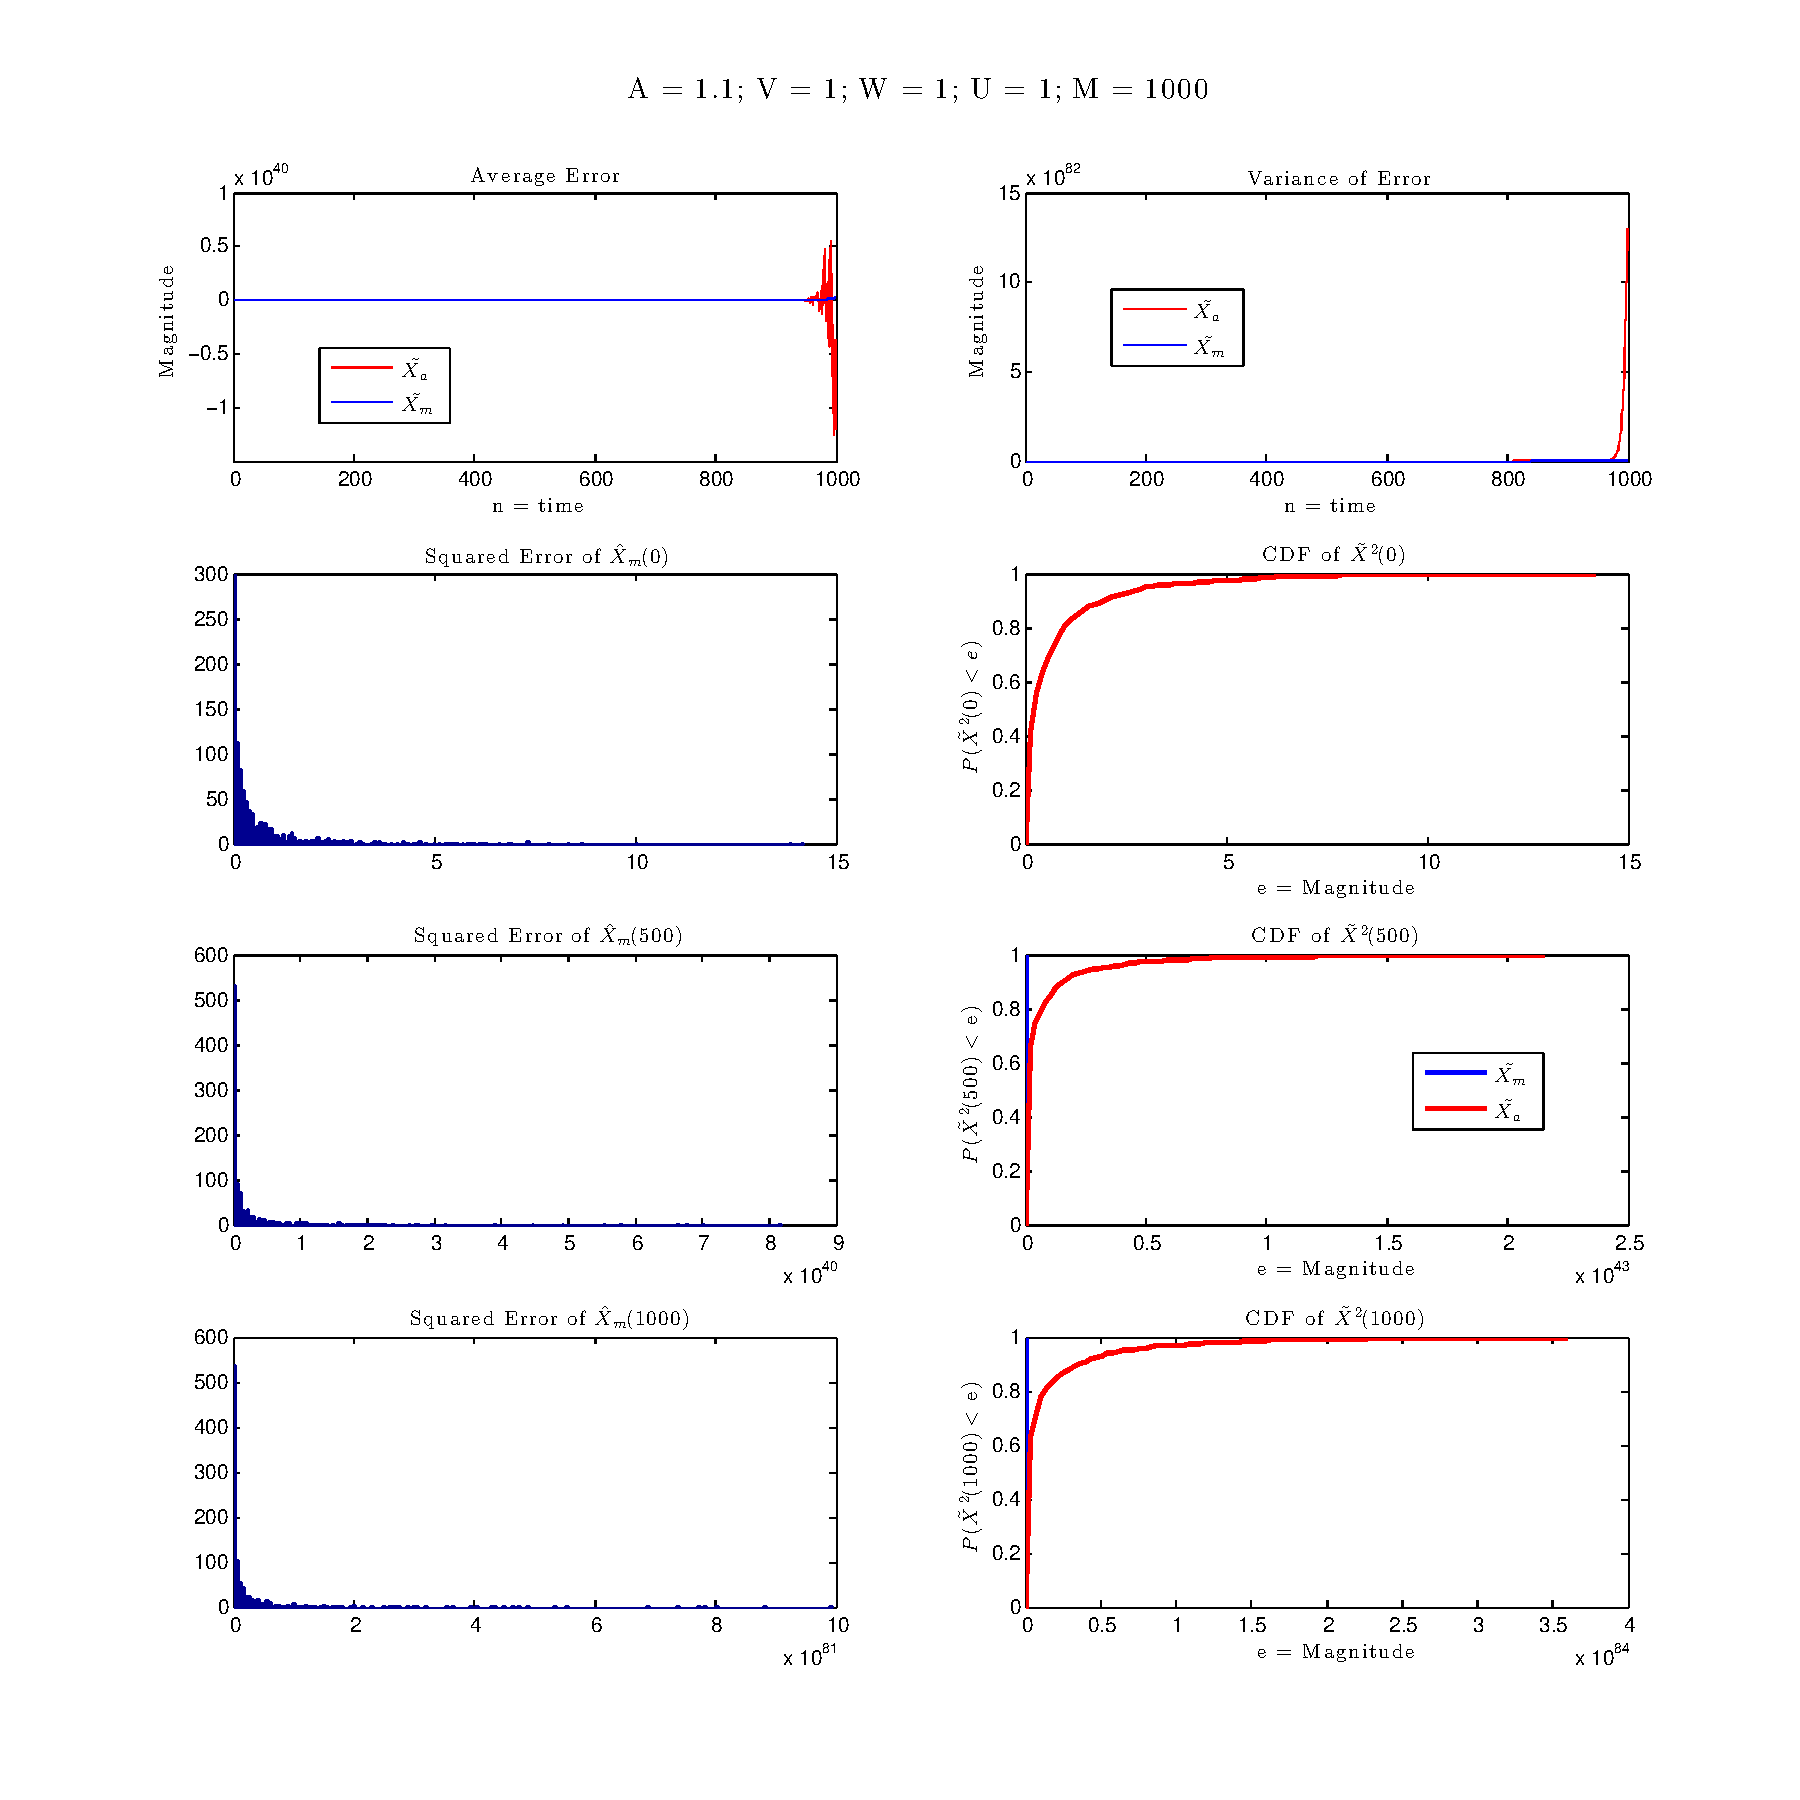
\includegraphics[width=\textwidth]{/Users/leahdickstein/Dropbox/R.edu/Sahai/140706/kfmul_a11_m1000}
\end{minipage}
\begin{minipage}[c]{0.5\textwidth}
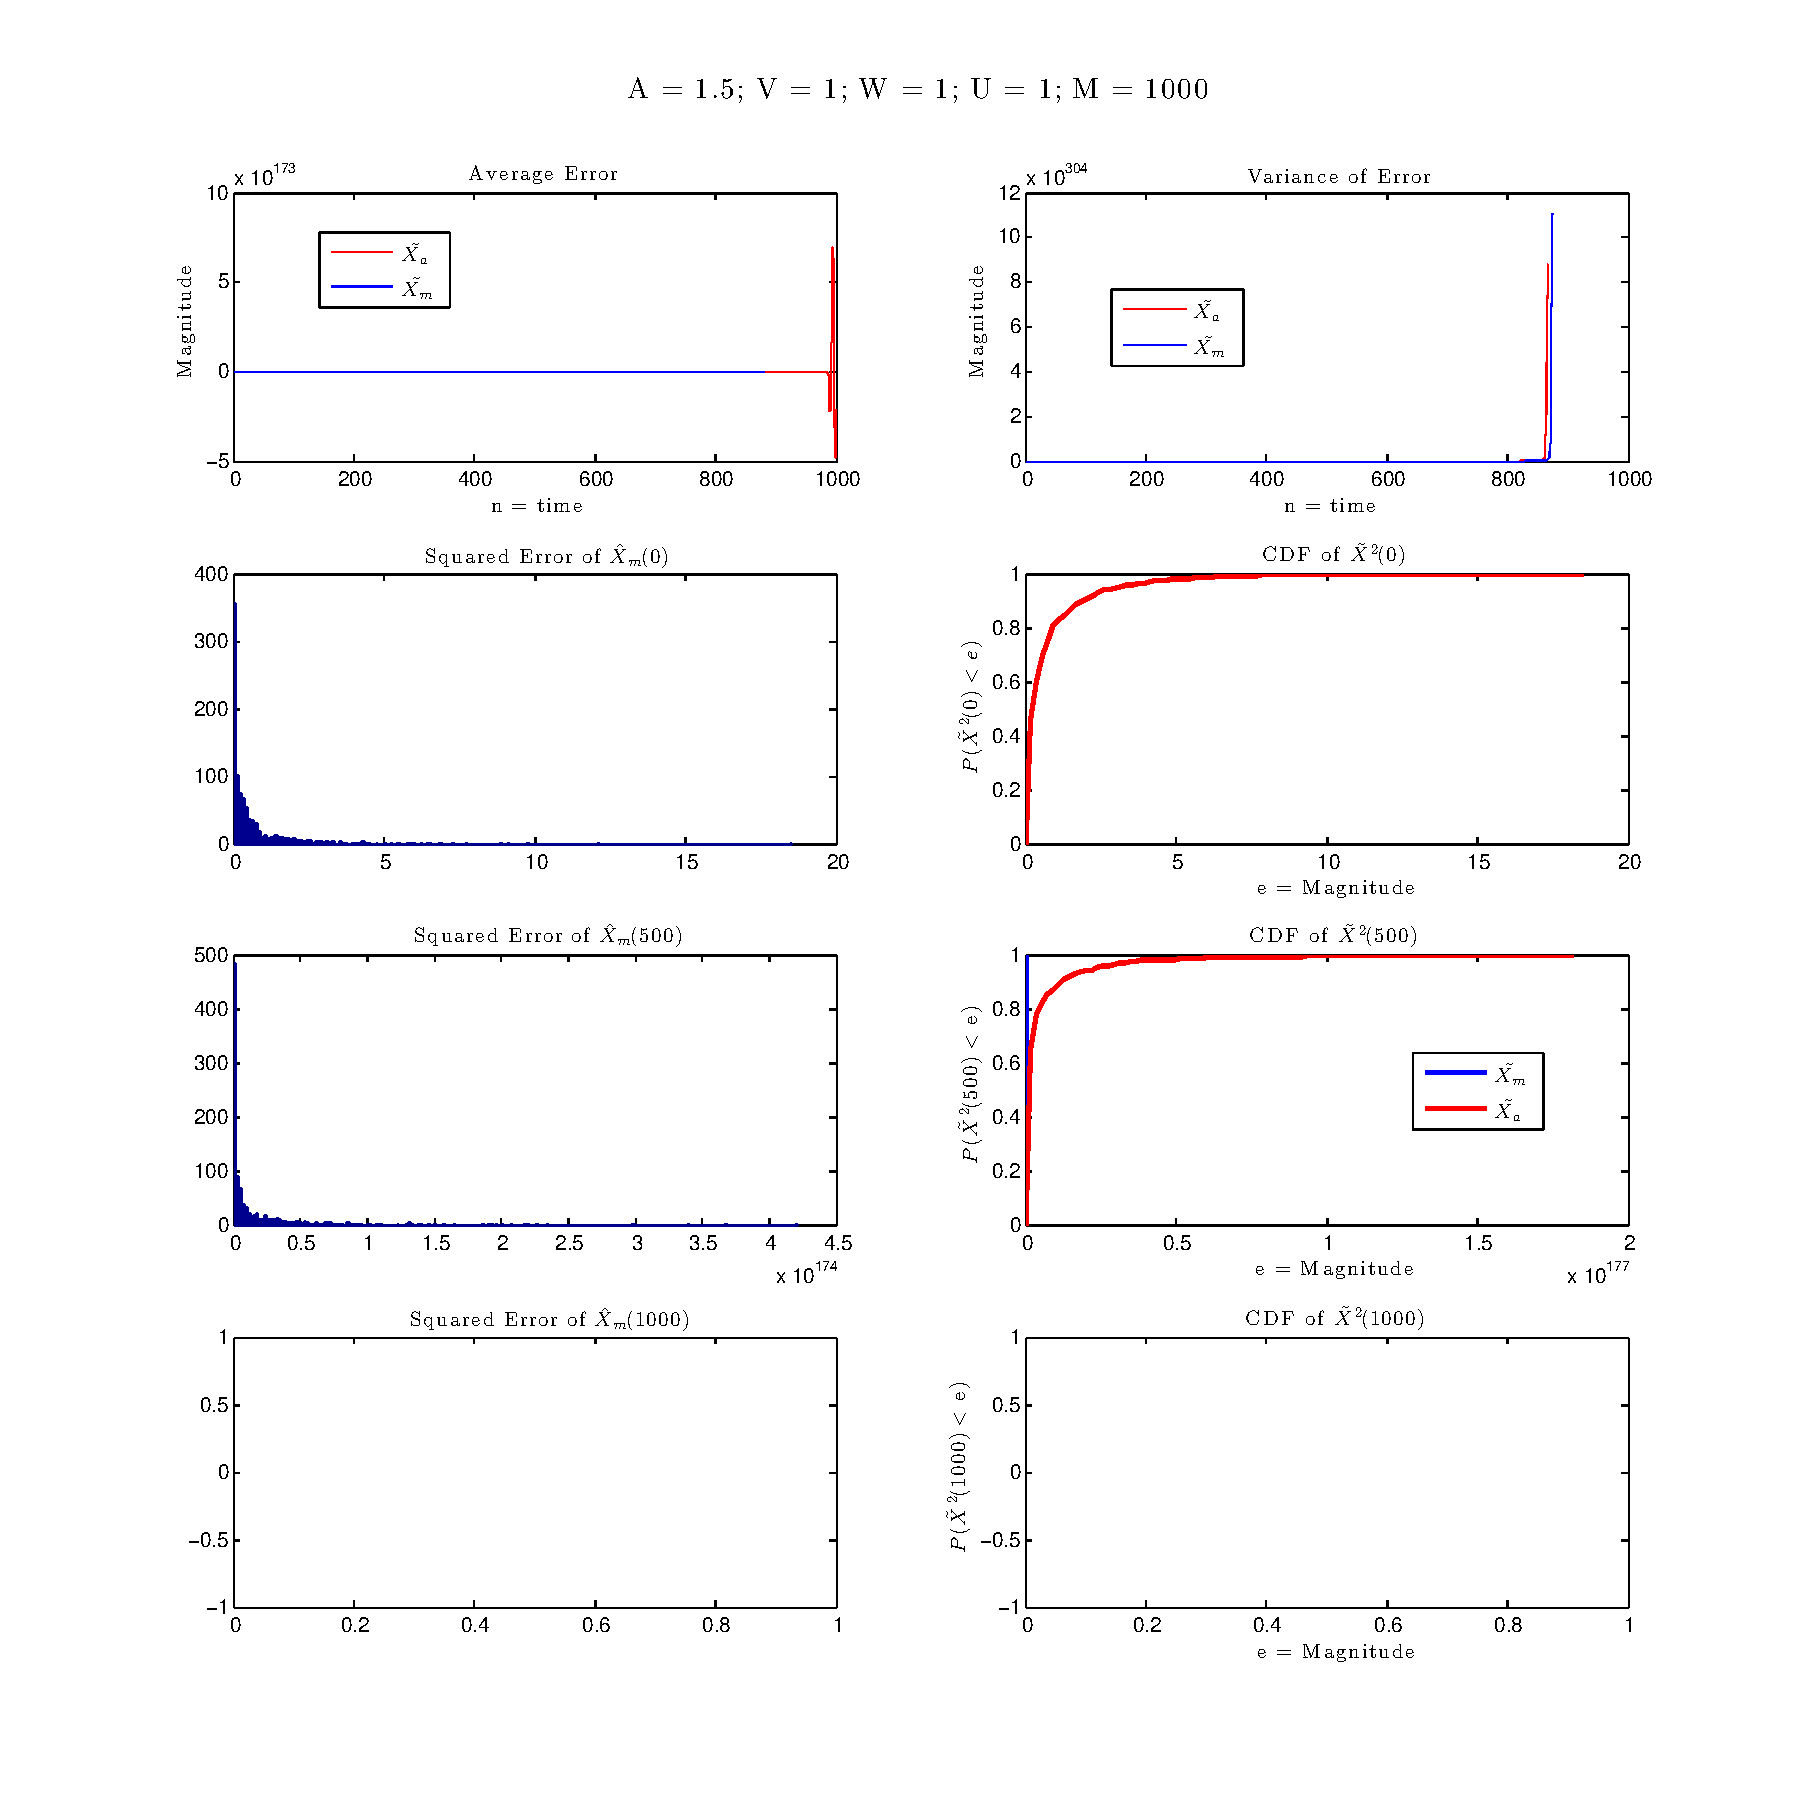
\includegraphics[width=\textwidth]{/Users/leahdickstein/Dropbox/R.edu/Sahai/140706/kfmul_a15_m1000}
\end{minipage}

This is the implementation of a Kalman Filter for Multiplicative Noise (Rajasekaran) with a system that has both multiplicative and additive noise. $\tilde{X}_a$ represents the estimation error for a Kalman Filter for only additive noise, while $\tilde{X}_m$ represents the new Kalman Filter. It is apparent the new Kalman Filter is doing much better; both have bounded error variances, but $\tilde{X}_m$ is significantly lower.\\\\
In the upper left corner, A = 0.99. Since A $<$ 1, the state converges toward 0 and the estimation error variance for $X_a$ is bounded. That being said, Var($\tilde{X}_m$) is still better (bounded at a lower value) than Var($\tilde{X}_a$). In the upper right, A = 1. Var($\tilde{X}_a$) matches the behavior we would expect, which is increasing linearly similar to the previous "Ignoring Multiplicative Noise with A = 1" plots above. Var($\tilde{X}_m$) is bounded, again as we would expect since we're using a Kalman Filter intended for multiplicative noise. In the lower left, A = 1.1. In this case, you can see the estimation error variance explodes, with Var($\tilde{X}_a$) increasing up to $10^82$. Var($\tilde{X}_m$), on the other hand, remains at its low bounded value. In the lower right, A = 1.5. The system is growing too fast over n = 1000 timesteps, and Matlab can't handle the numbers because they're getting too large. Both estimation error variances appear large because of value truncation/roundoff error done in Matlab. This simply means values $A > 1.5$ aren't testable in Matlab, even if Rajasekaran's Kalman Filter applies.

\subsection{Quantization Noise: Schenato}
\begin{minipage}[c]{0.5\textwidth}
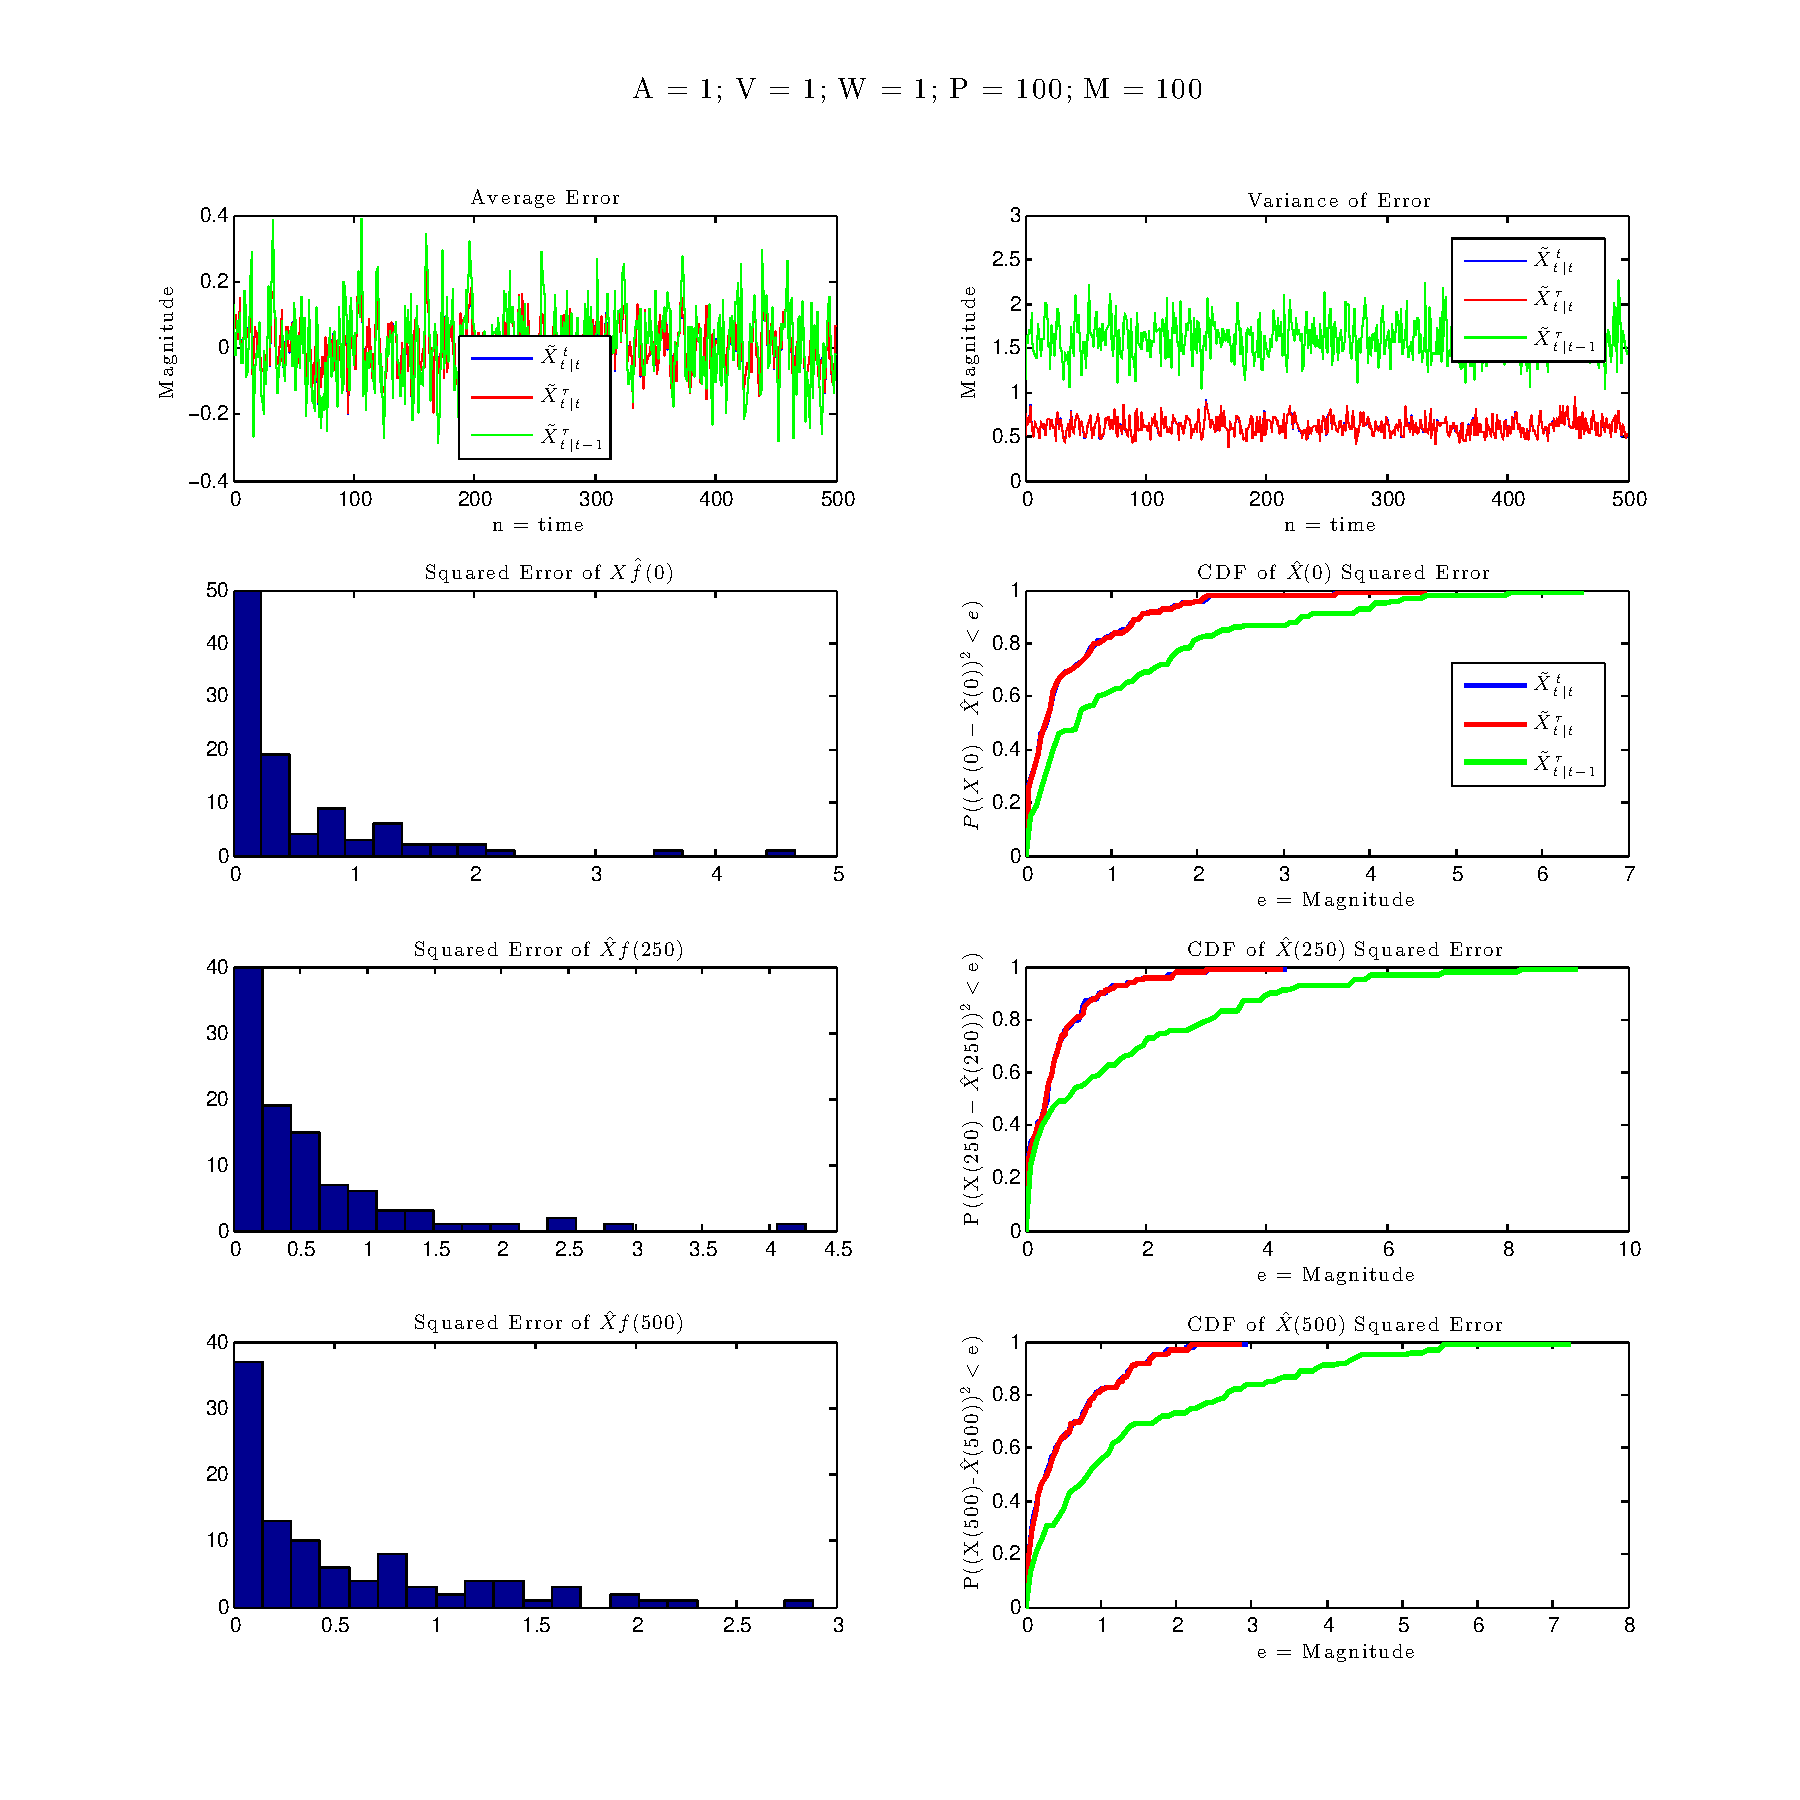
\includegraphics[width=\textwidth]{/Users/leahdickstein/Dropbox/R.edu/Sahai/140626/fig3_p100_m100}
\end{minipage}
\begin{minipage}[c]{0.5\textwidth}
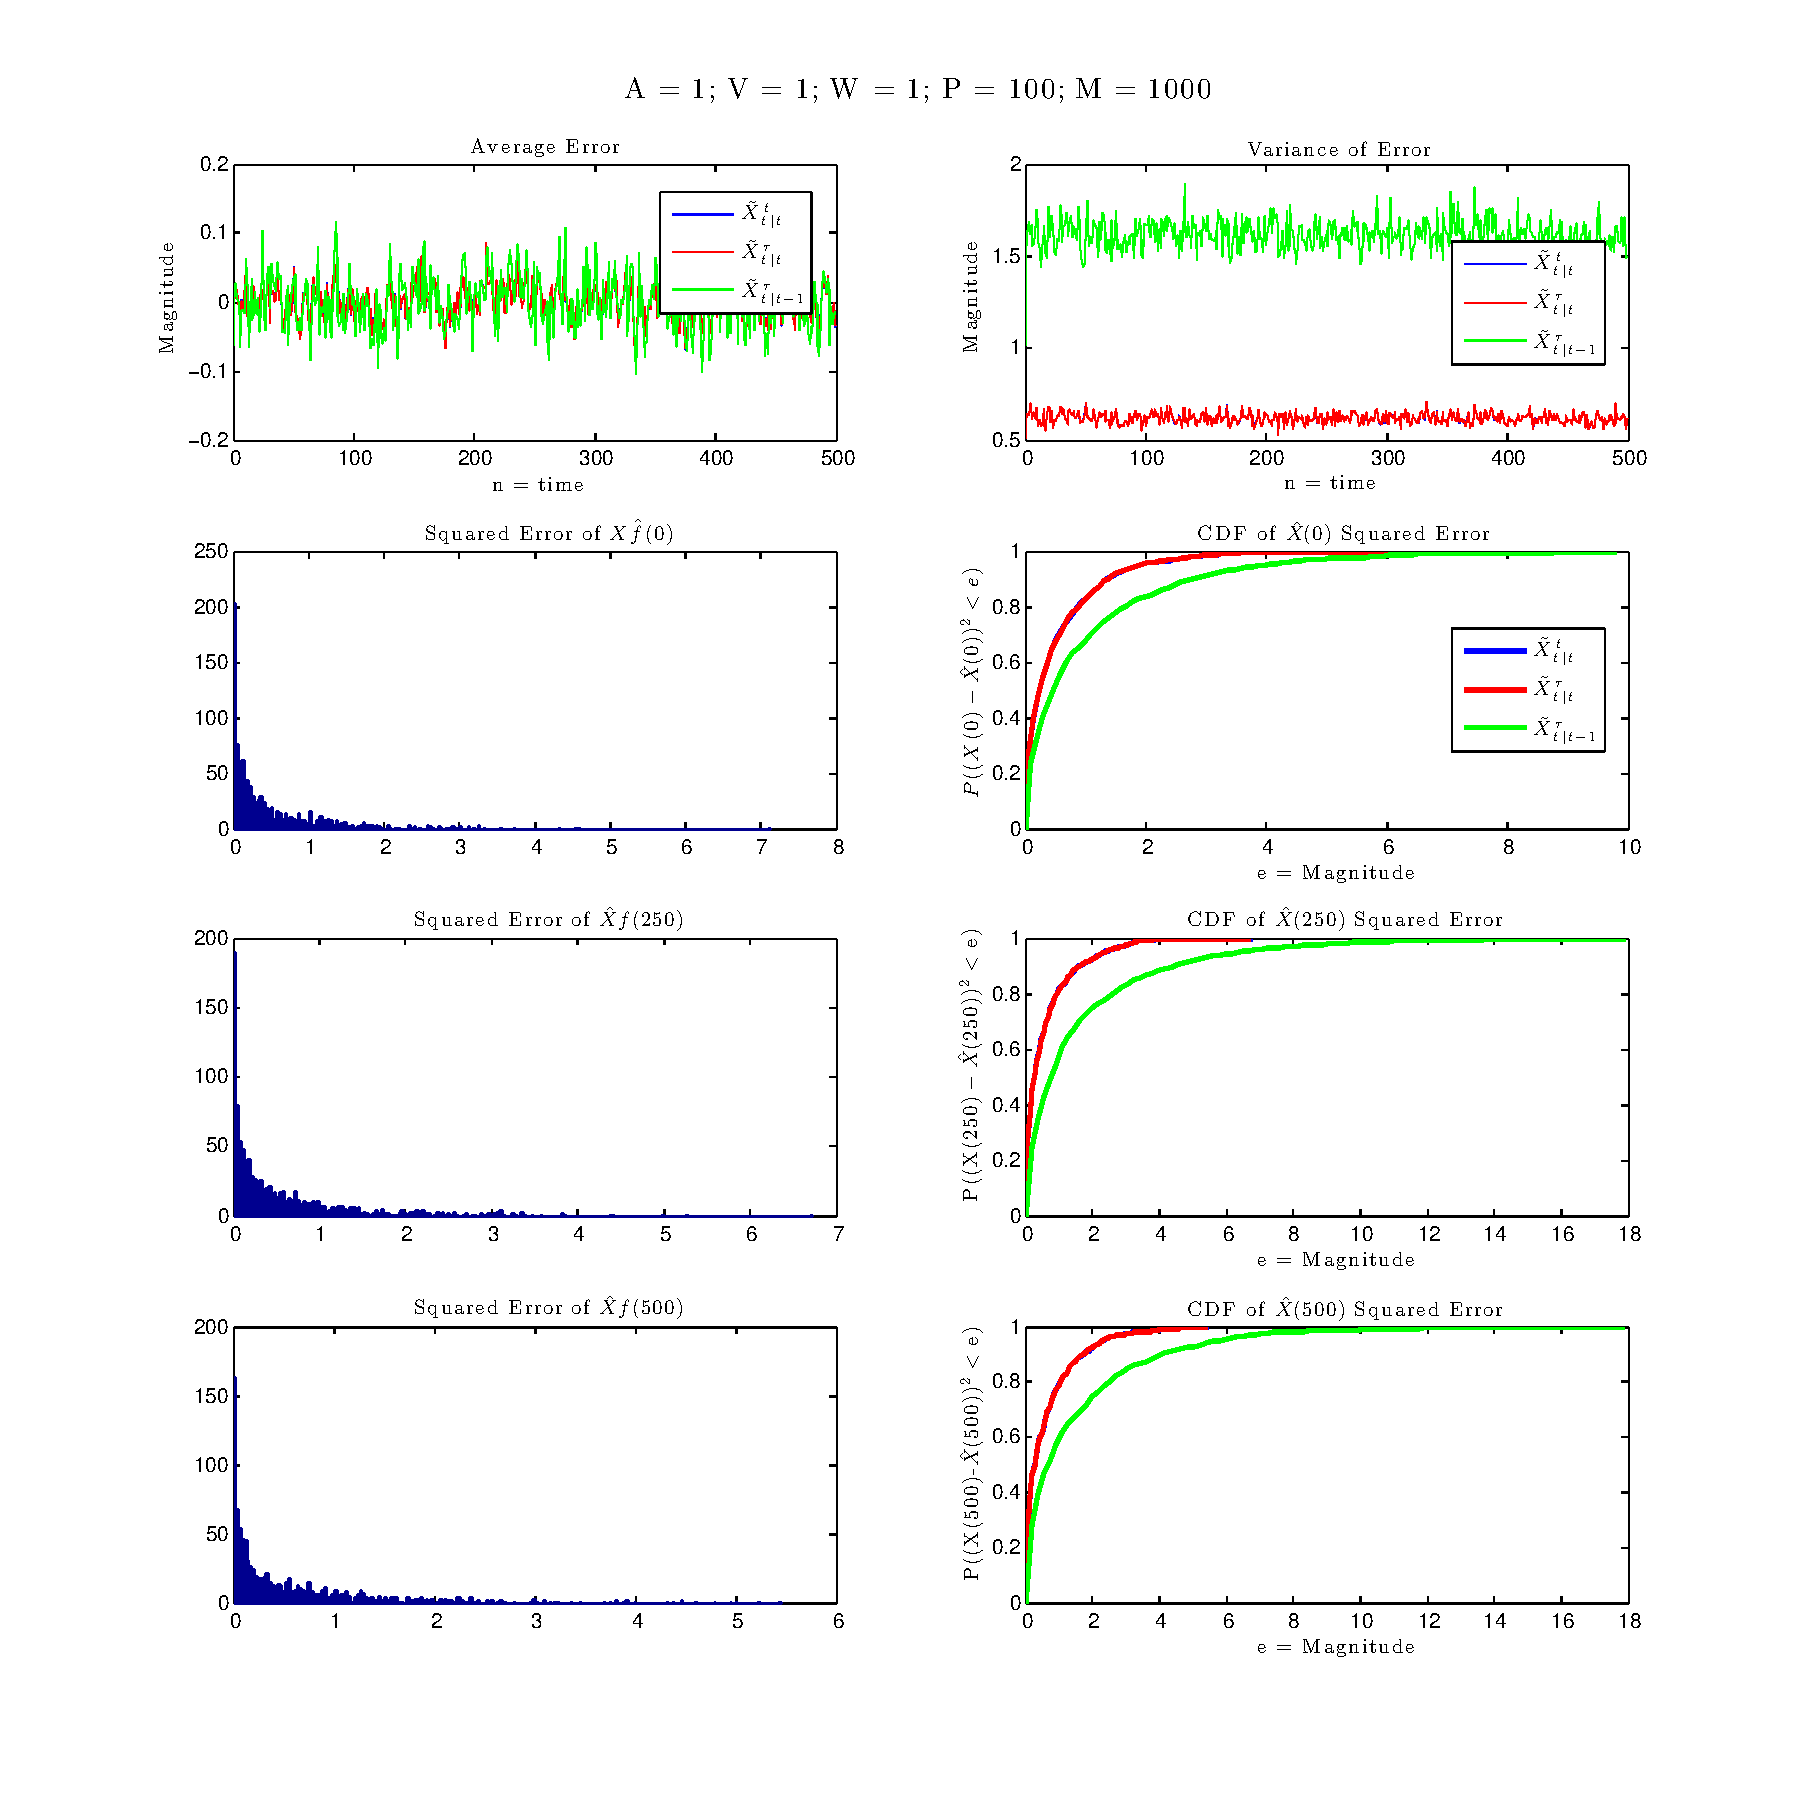
\includegraphics[width=\textwidth]{/Users/leahdickstein/Dropbox/R.edu/Sahai/140626/fig3_p100_m1000}
\end{minipage}

\begin{minipage}[c]{0.5\textwidth}
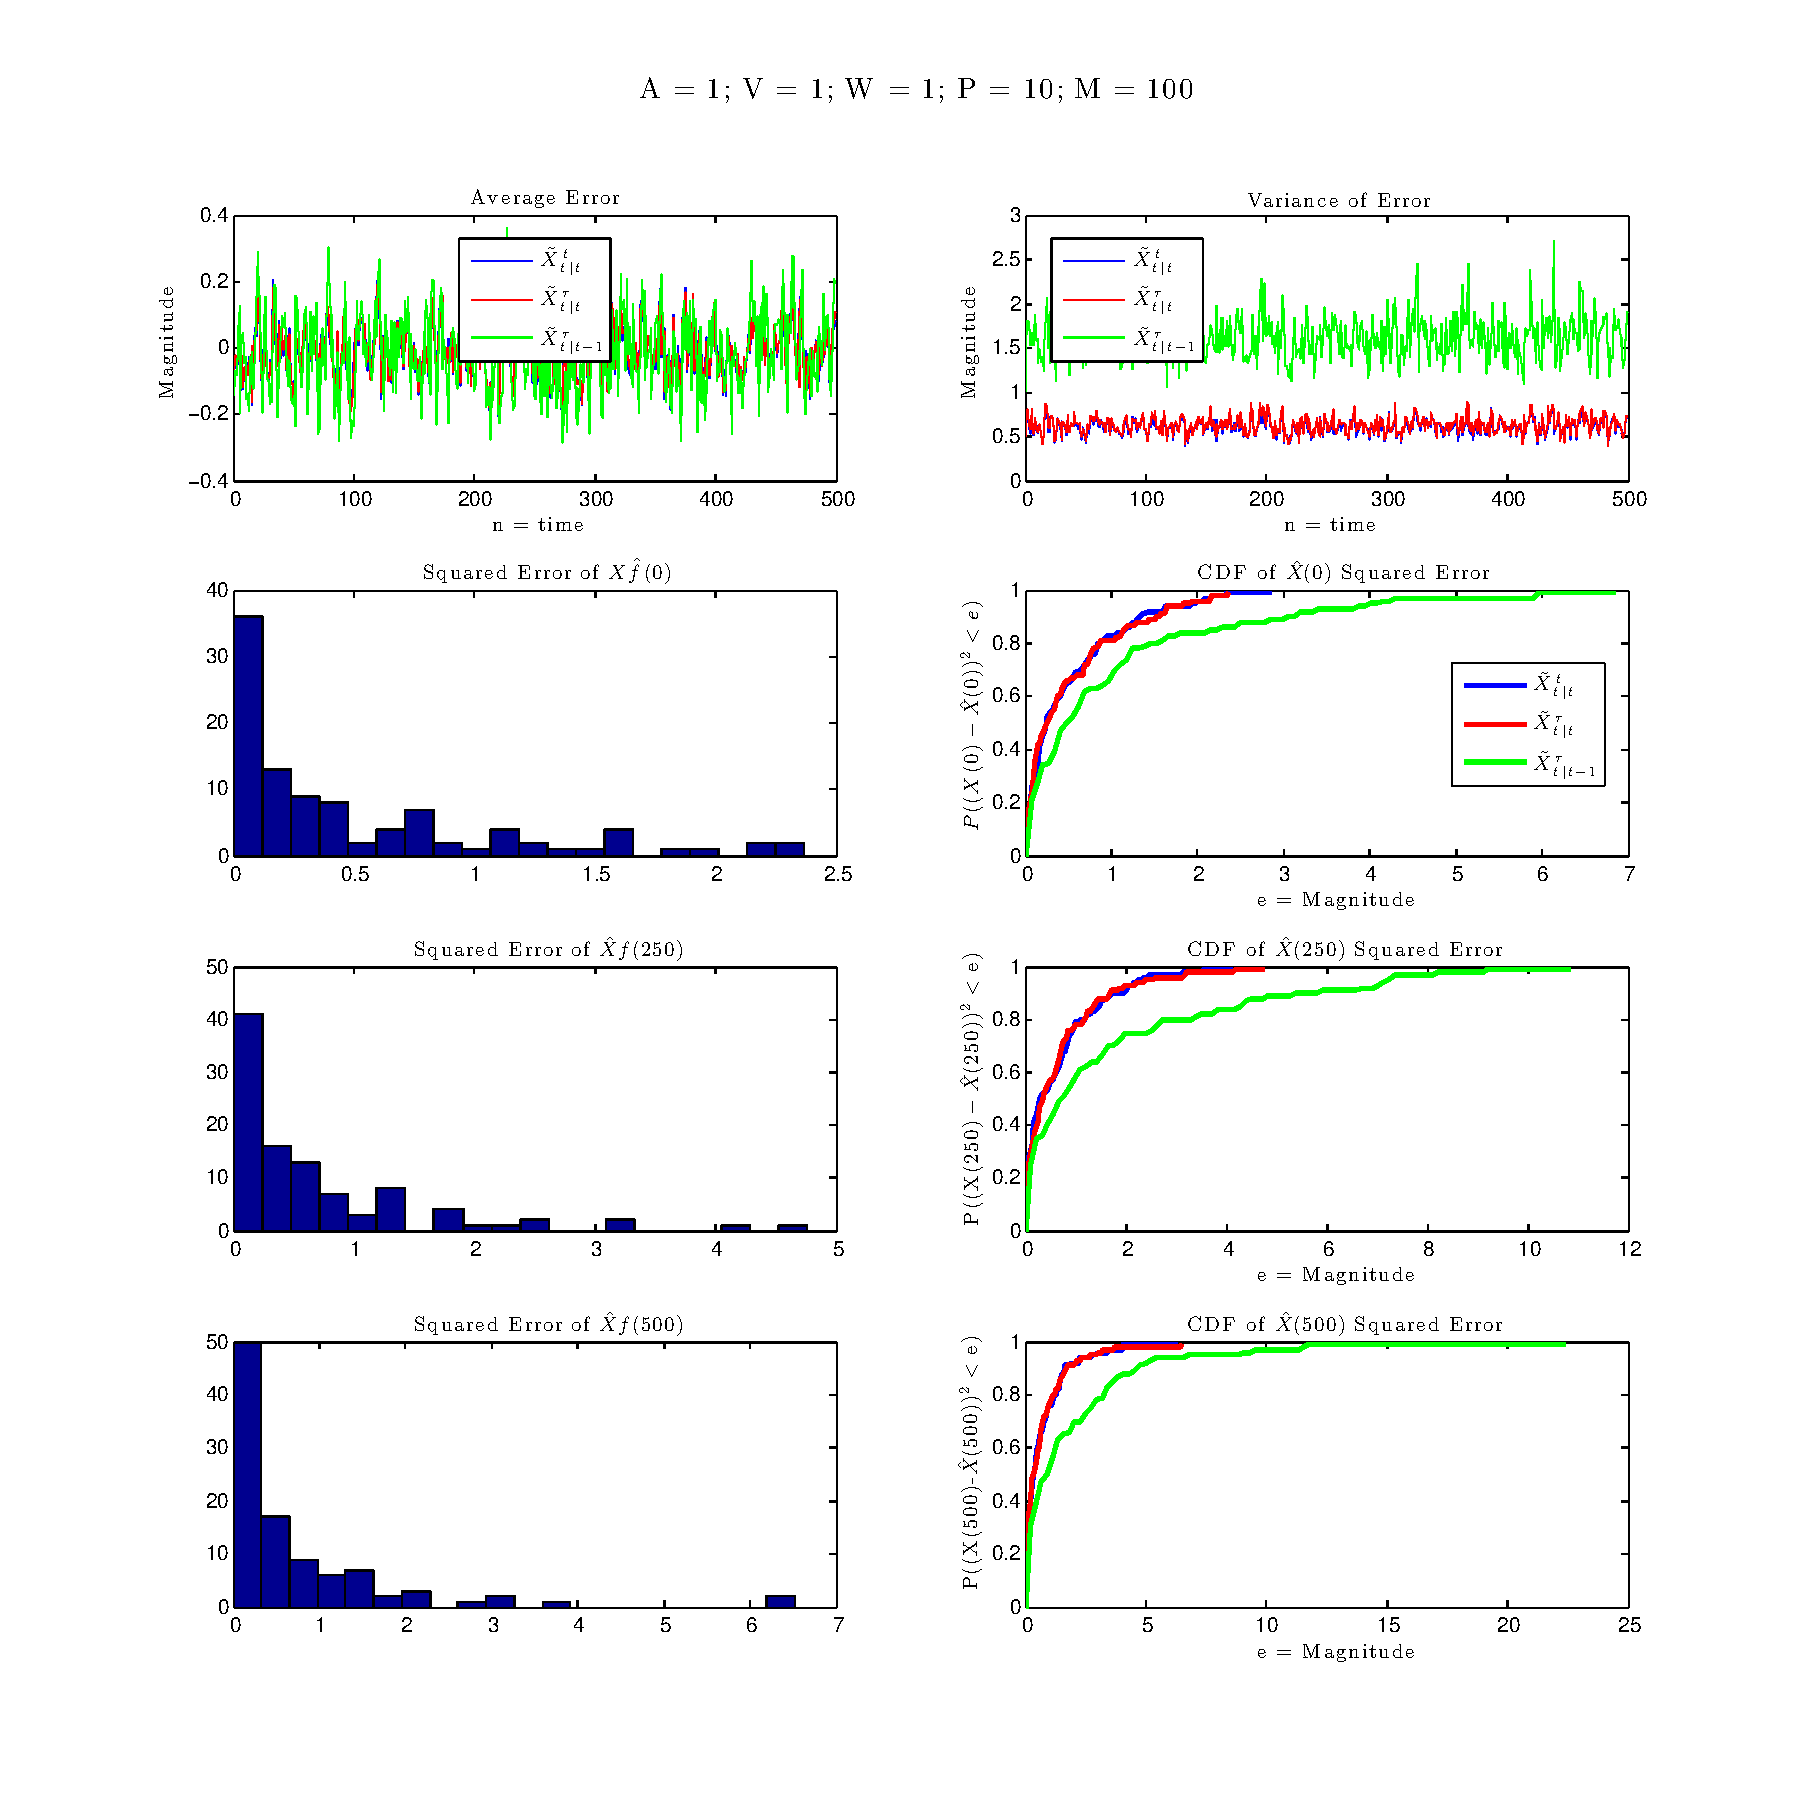
\includegraphics[width=\textwidth]{/Users/leahdickstein/Dropbox/R.edu/Sahai/140626/fig3_p10_m100}
\end{minipage}
\begin{minipage}[c]{0.5\textwidth}
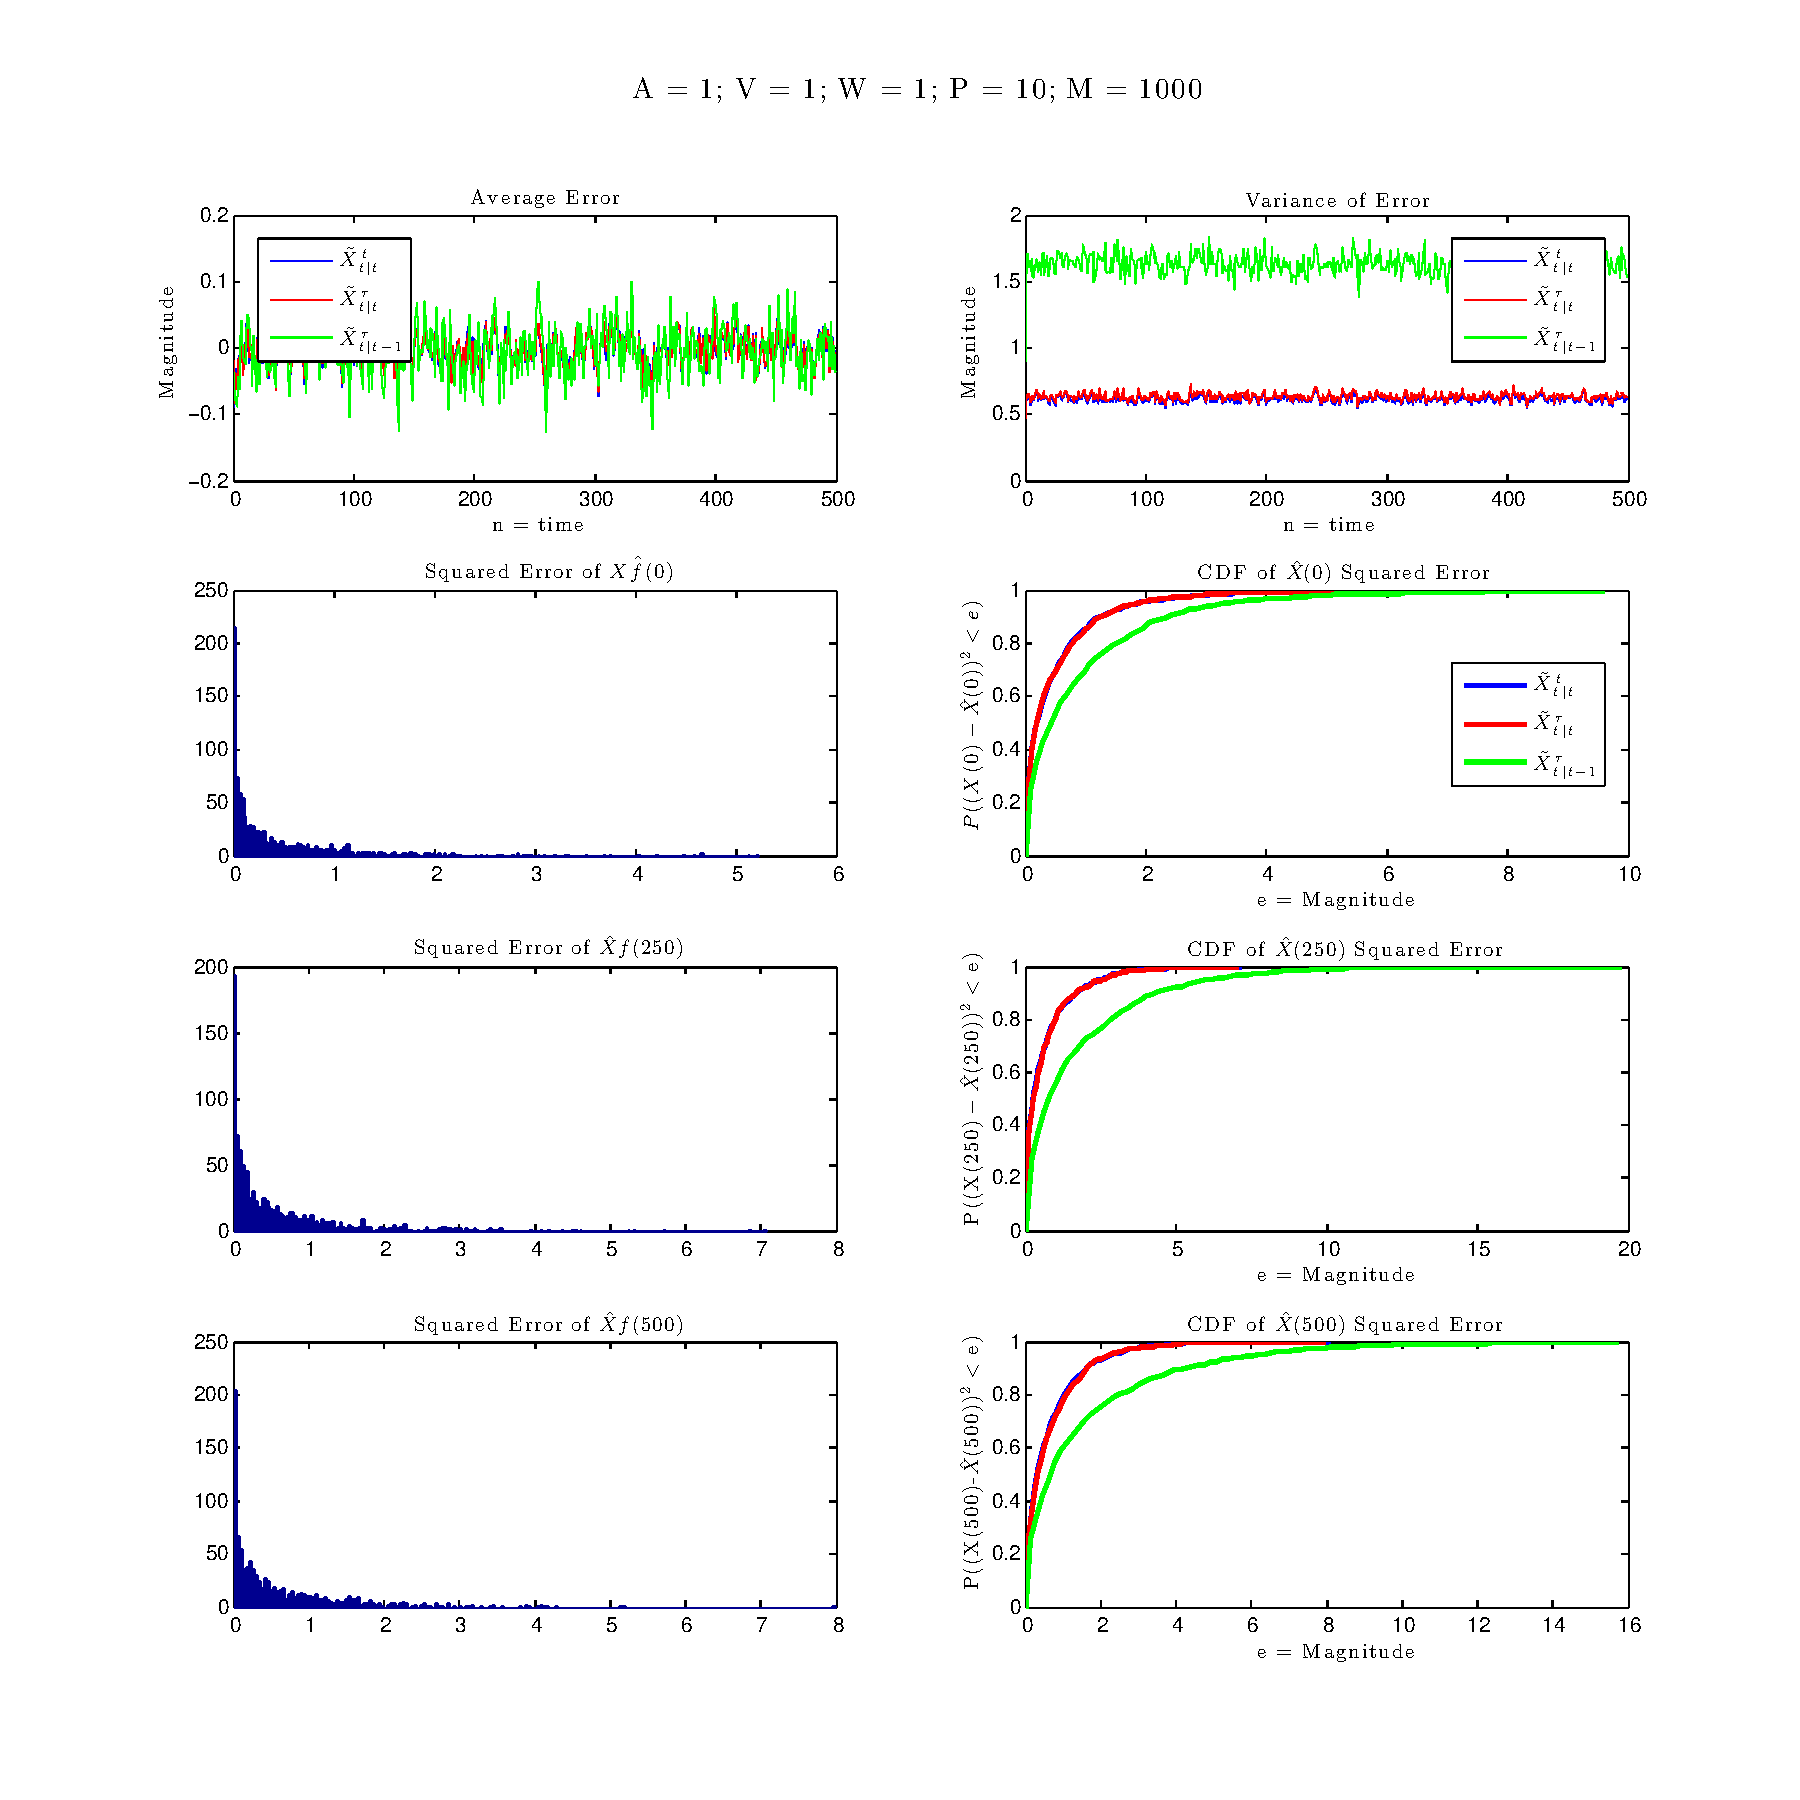
\includegraphics[width=\textwidth]{/Users/leahdickstein/Dropbox/R.edu/Sahai/140626/fig3_p10_m1000}
\end{minipage}

\begin{minipage}[c]{0.5\textwidth}
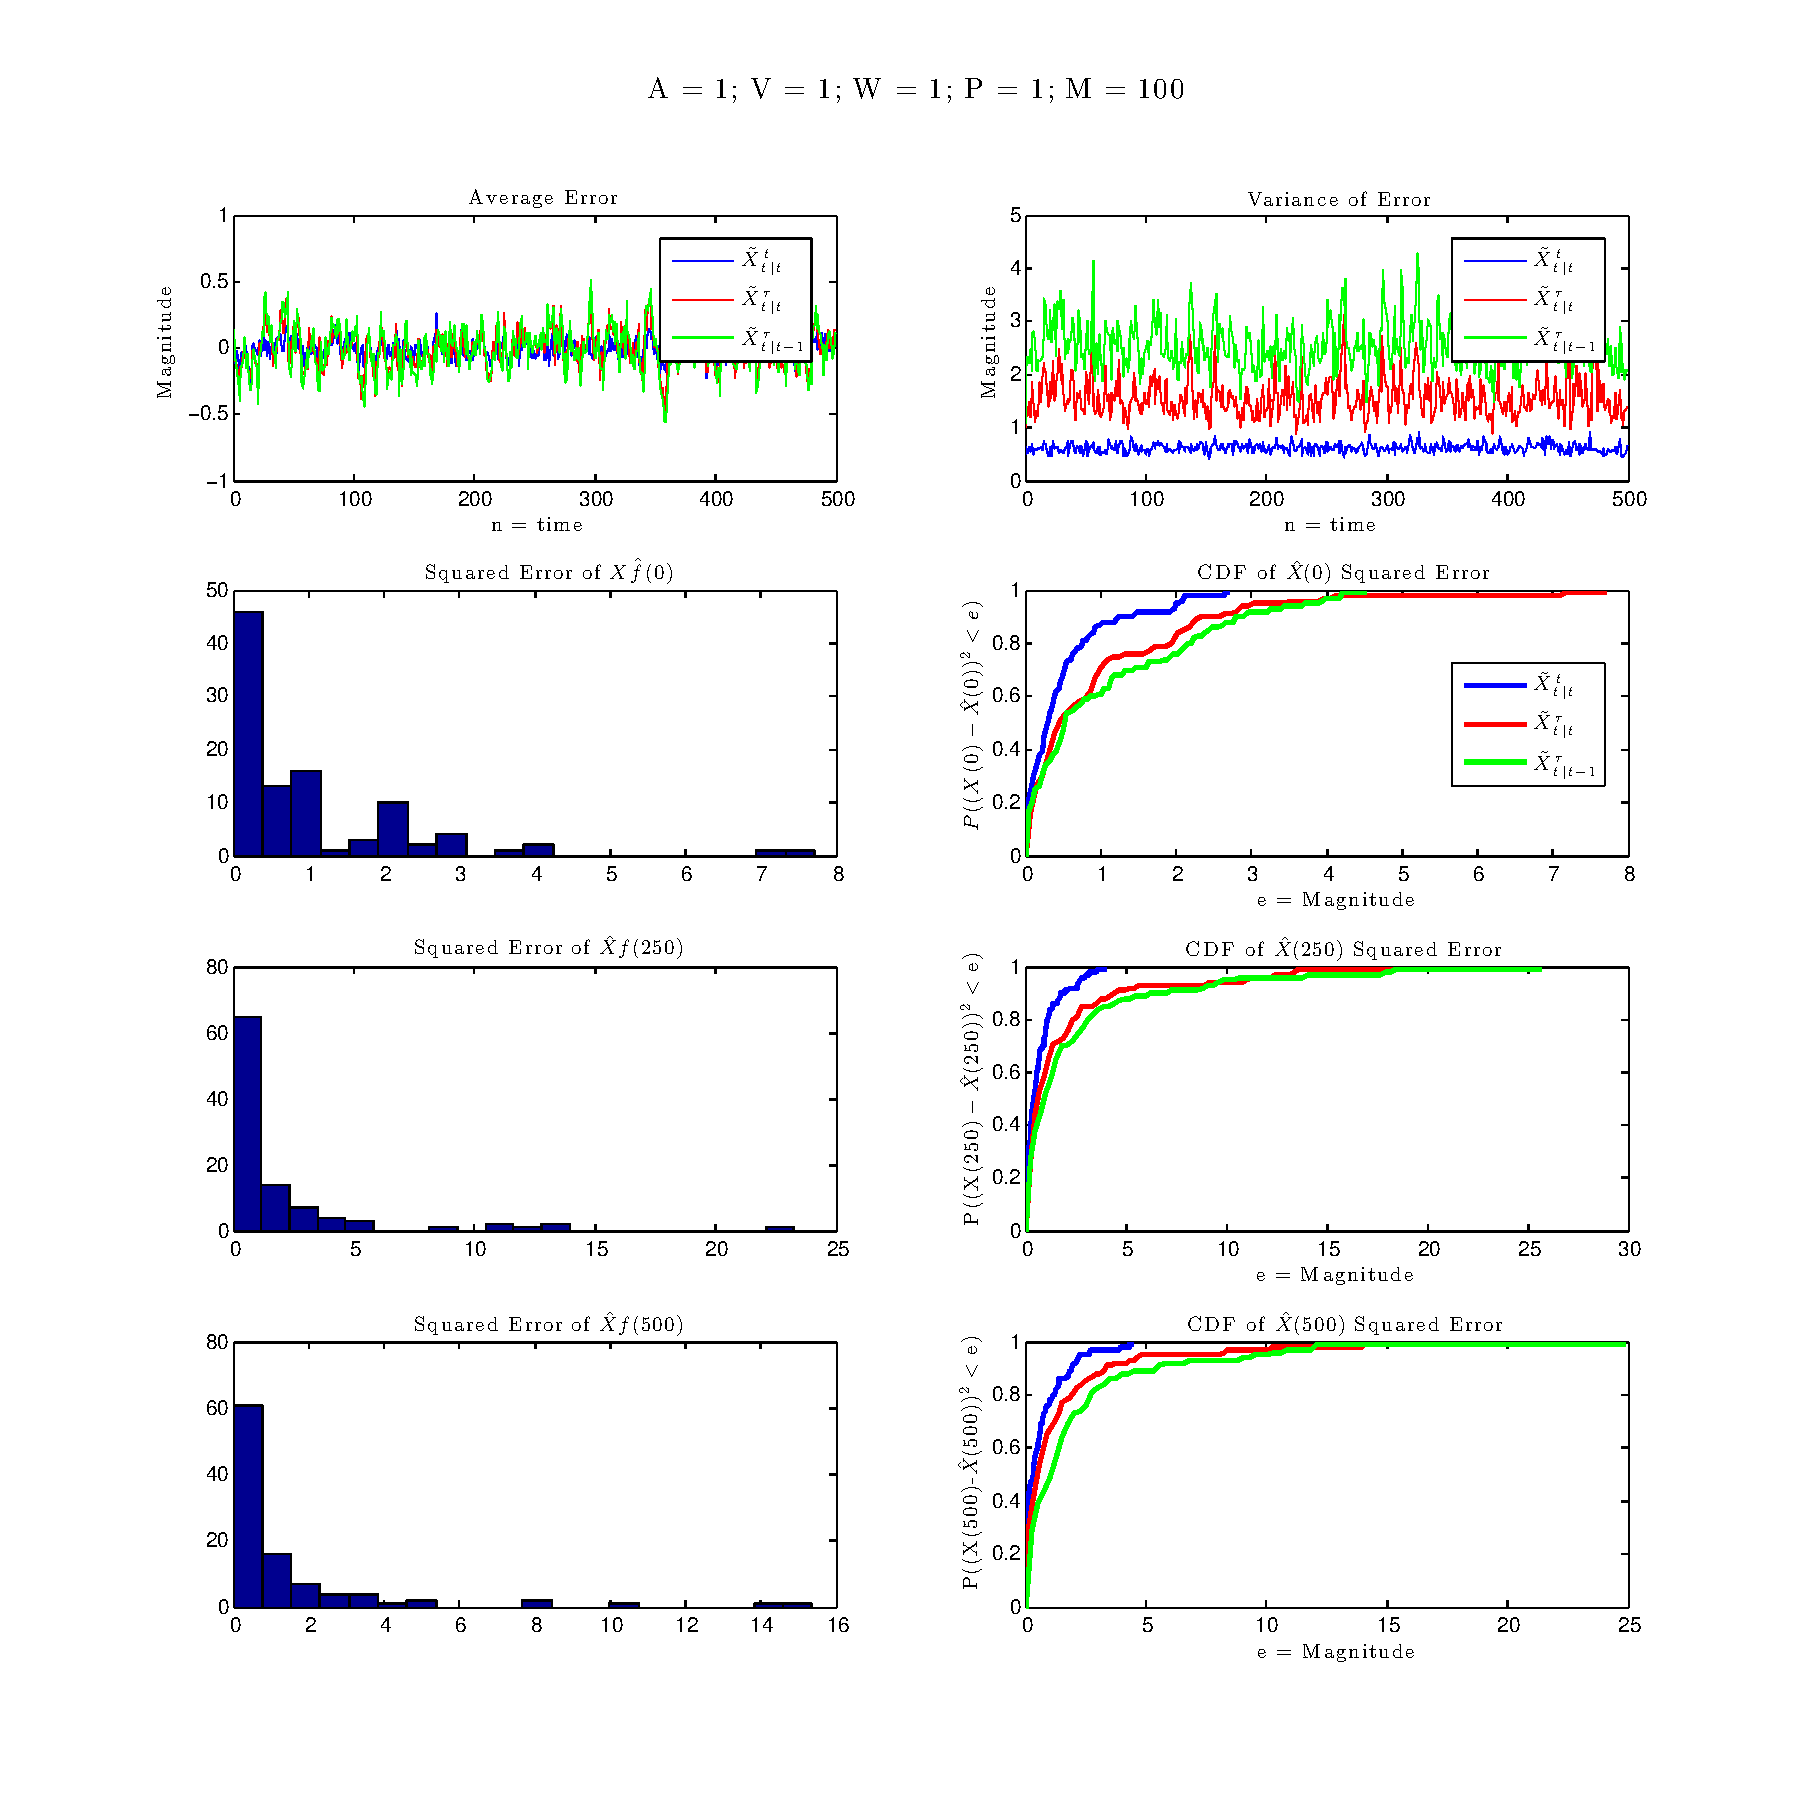
\includegraphics[width=\textwidth]{/Users/leahdickstein/Dropbox/R.edu/Sahai/140626/fig3_p1_m100}
\end{minipage}
\begin{minipage}[c]{0.5\textwidth}
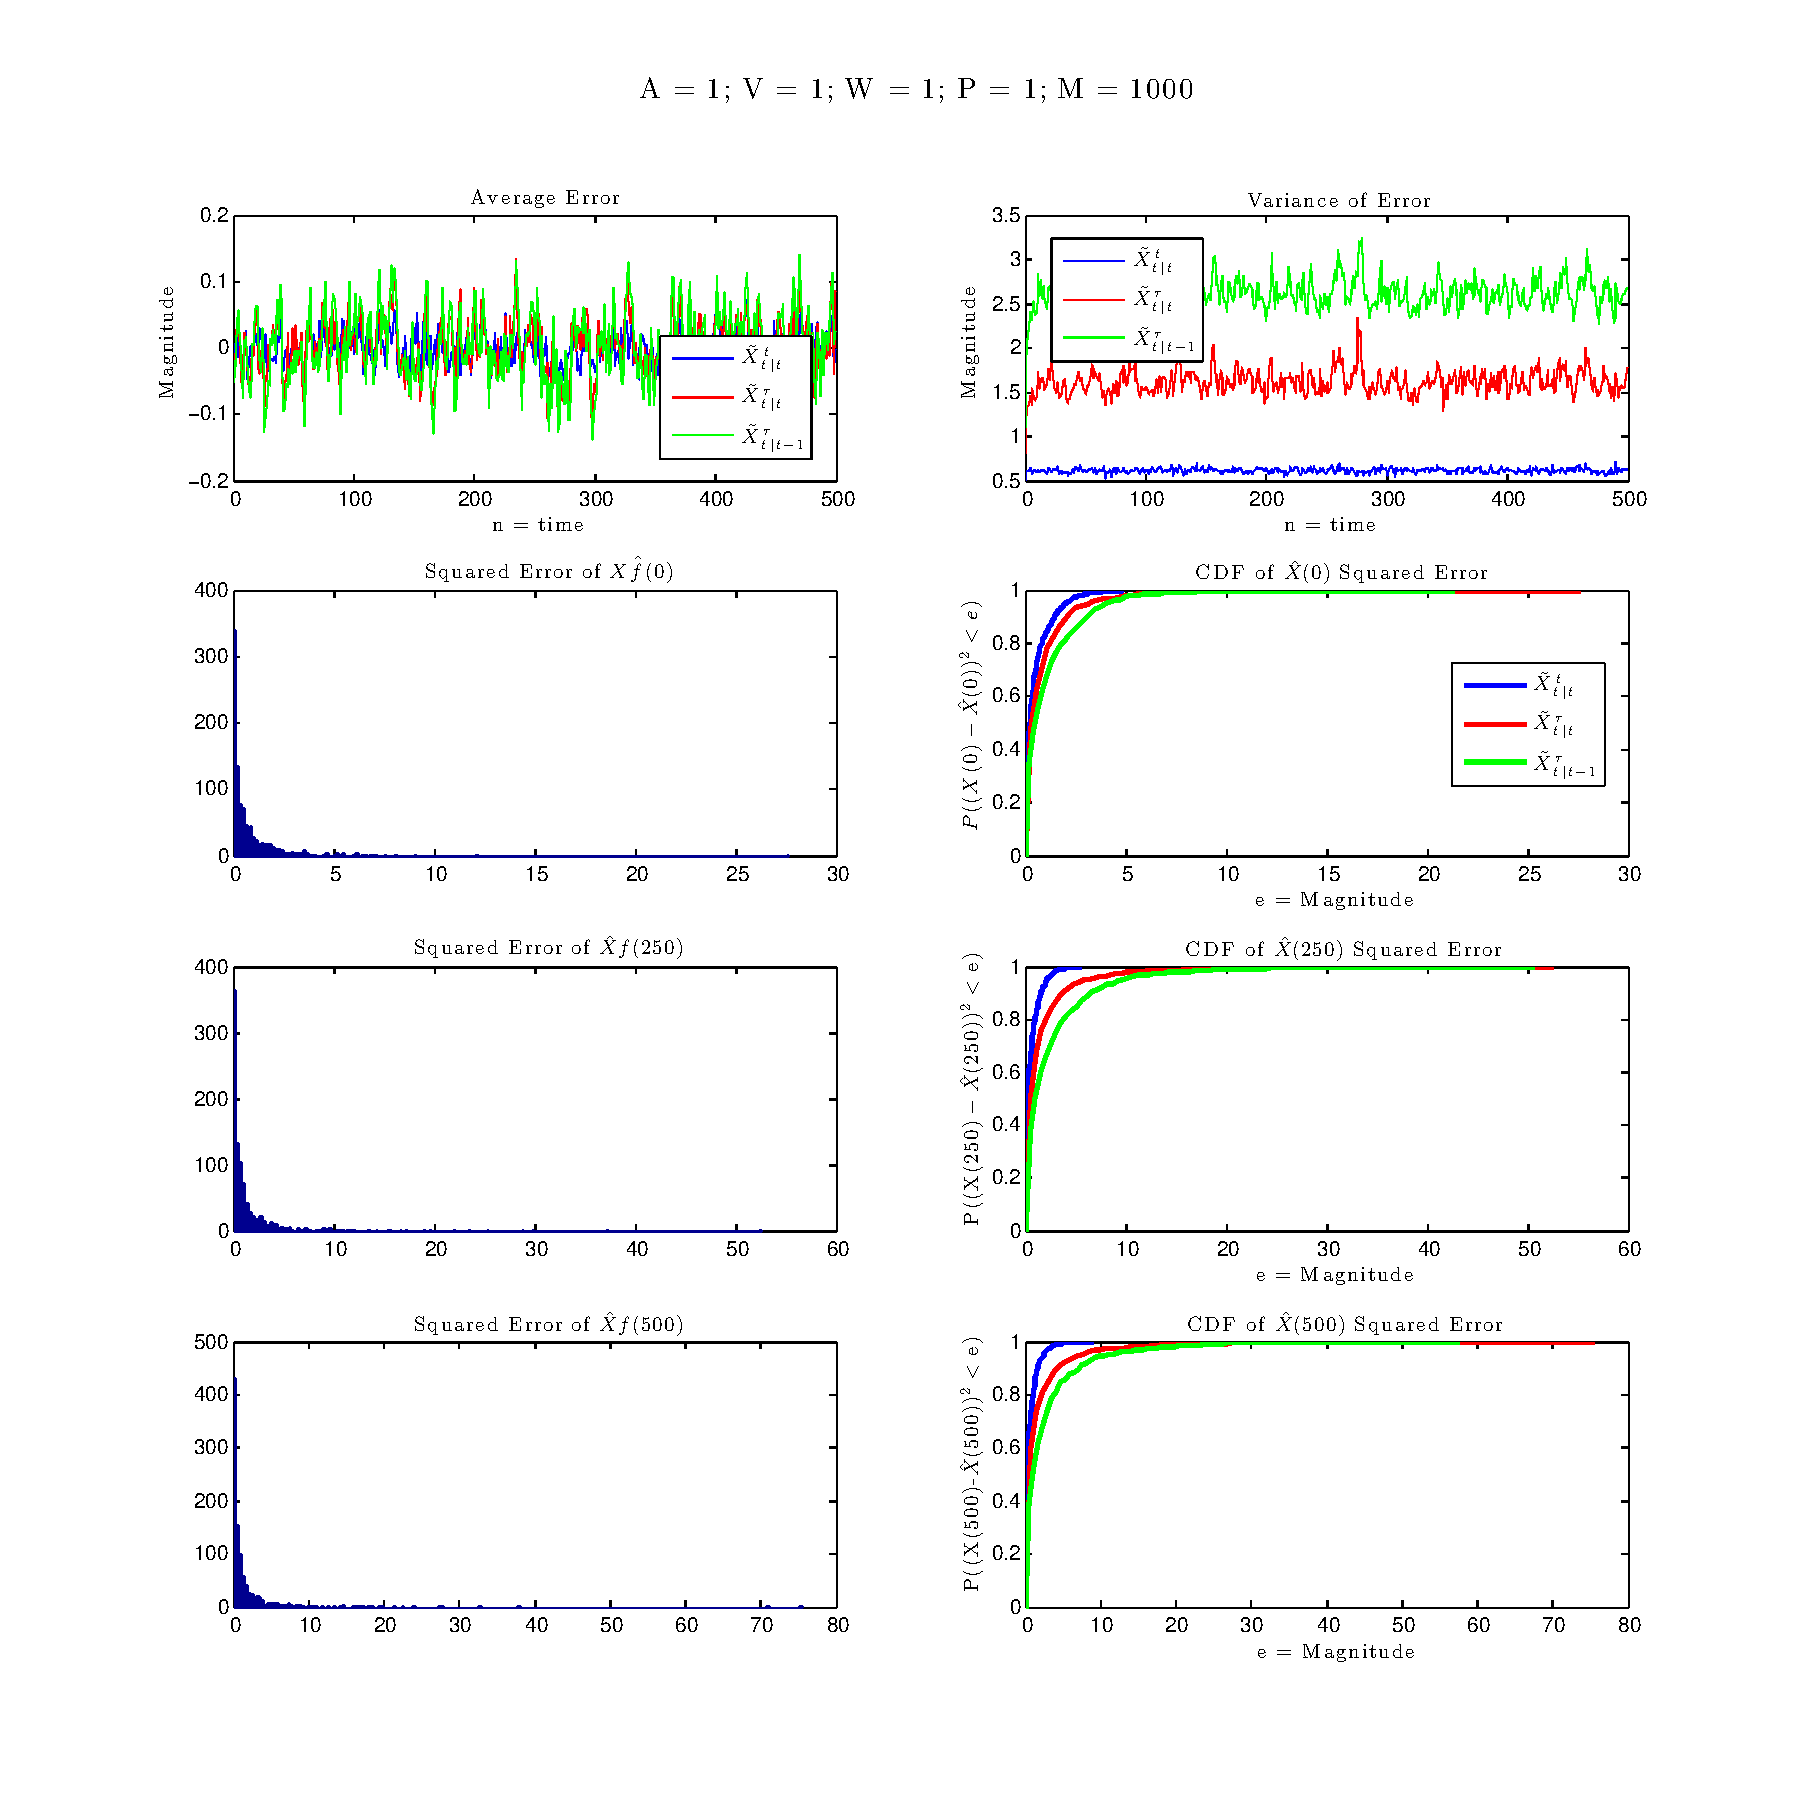
\includegraphics[width=\textwidth]{/Users/leahdickstein/Dropbox/R.edu/Sahai/140626/fig3_p1_m1000}
\end{minipage}

\begin{minipage}[c]{0.5\textwidth}
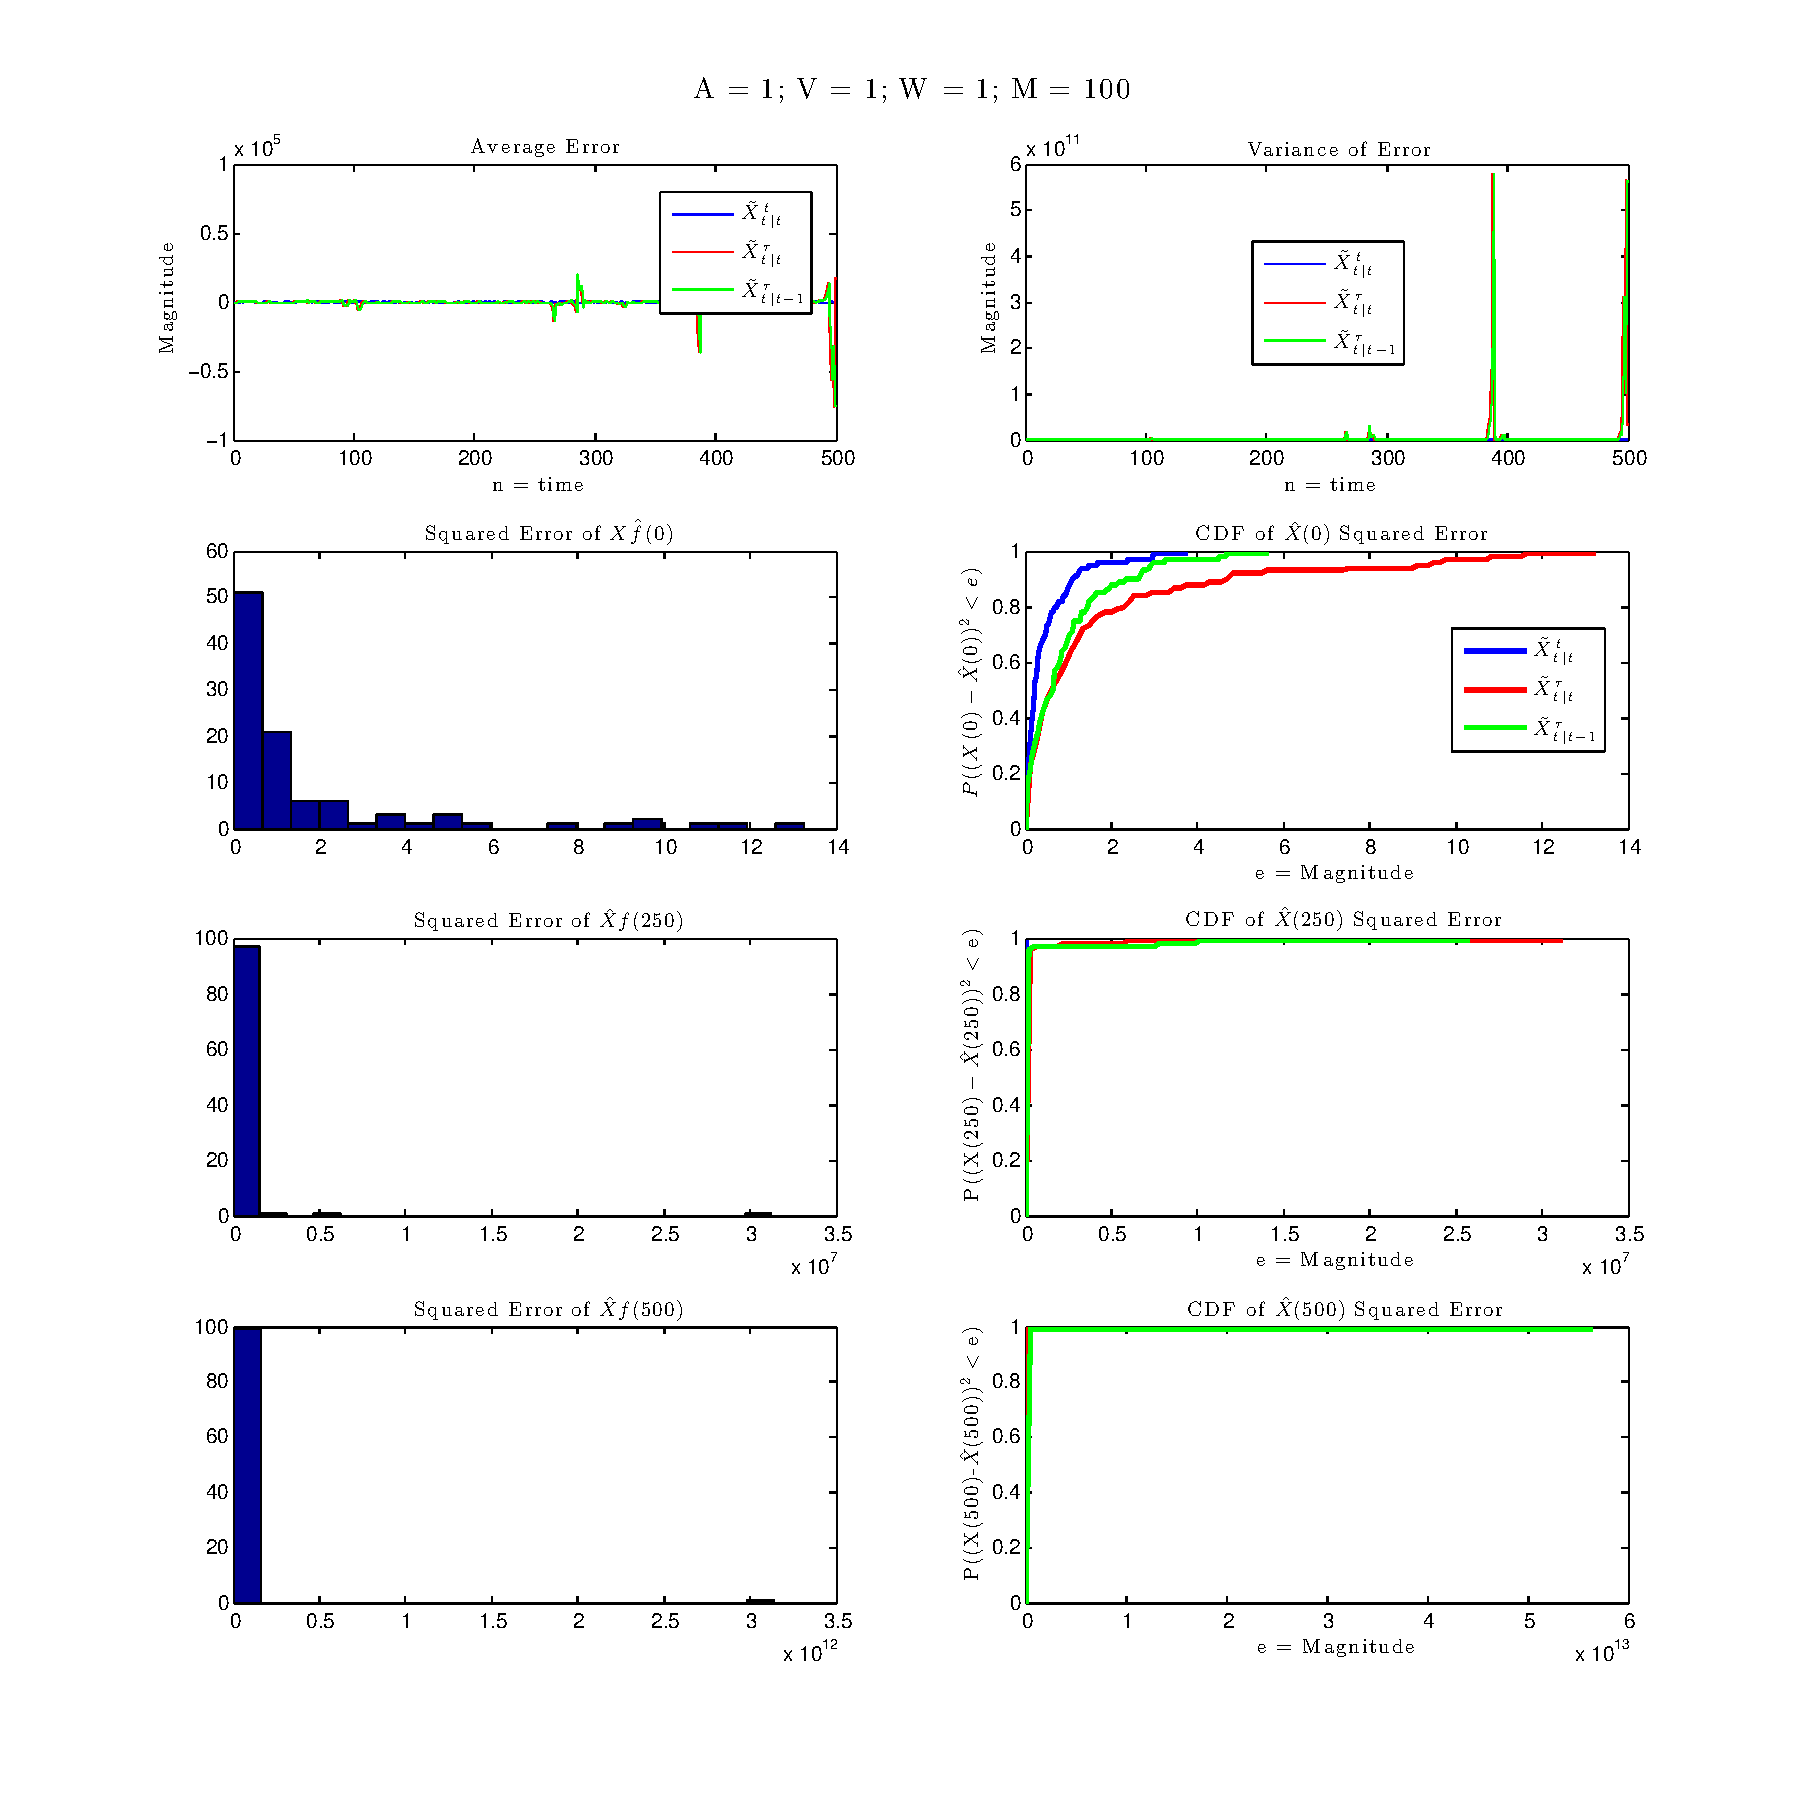
\includegraphics[width=\textwidth]{/Users/leahdickstein/Dropbox/R.edu/Sahai/140626/fig3_p001_m100}
\end{minipage}
\begin{minipage}[b]{0.5\textwidth}
These figures are the implementation of Schenato's paper, with multiplicative noise but no packet drops. Multiplicative (quantization) noise happens over the channel between the transmitter and the receiver. $\tilde{X}^t_{t|t}$ represents the transmitter's estimate of the state, using a Kalman Filter for additive noise (because so far there has only been additive noise.) $\tilde{X}^r_{t|t-1}$ represents a prediction of the state post-quantization noise, and $\tilde{X}^r_{t|t}$ represents the estimation of the state post-quantization noise. When the power is extremely small (thus the multiplicative noise has large variance), $\tilde{X}^r_{t|t-1}$ does better than $\tilde{X}^r_{t|t}$. This is because the multiplicative noise has such a huge effect, the prediction with the moderate growth A is closer to the real state than the totally inaccurate noisy signal.
\end{minipage}

\subsection{NonCoherence Estimation: Gireeja}
\begin{minipage}[c]{0.5\textwidth}
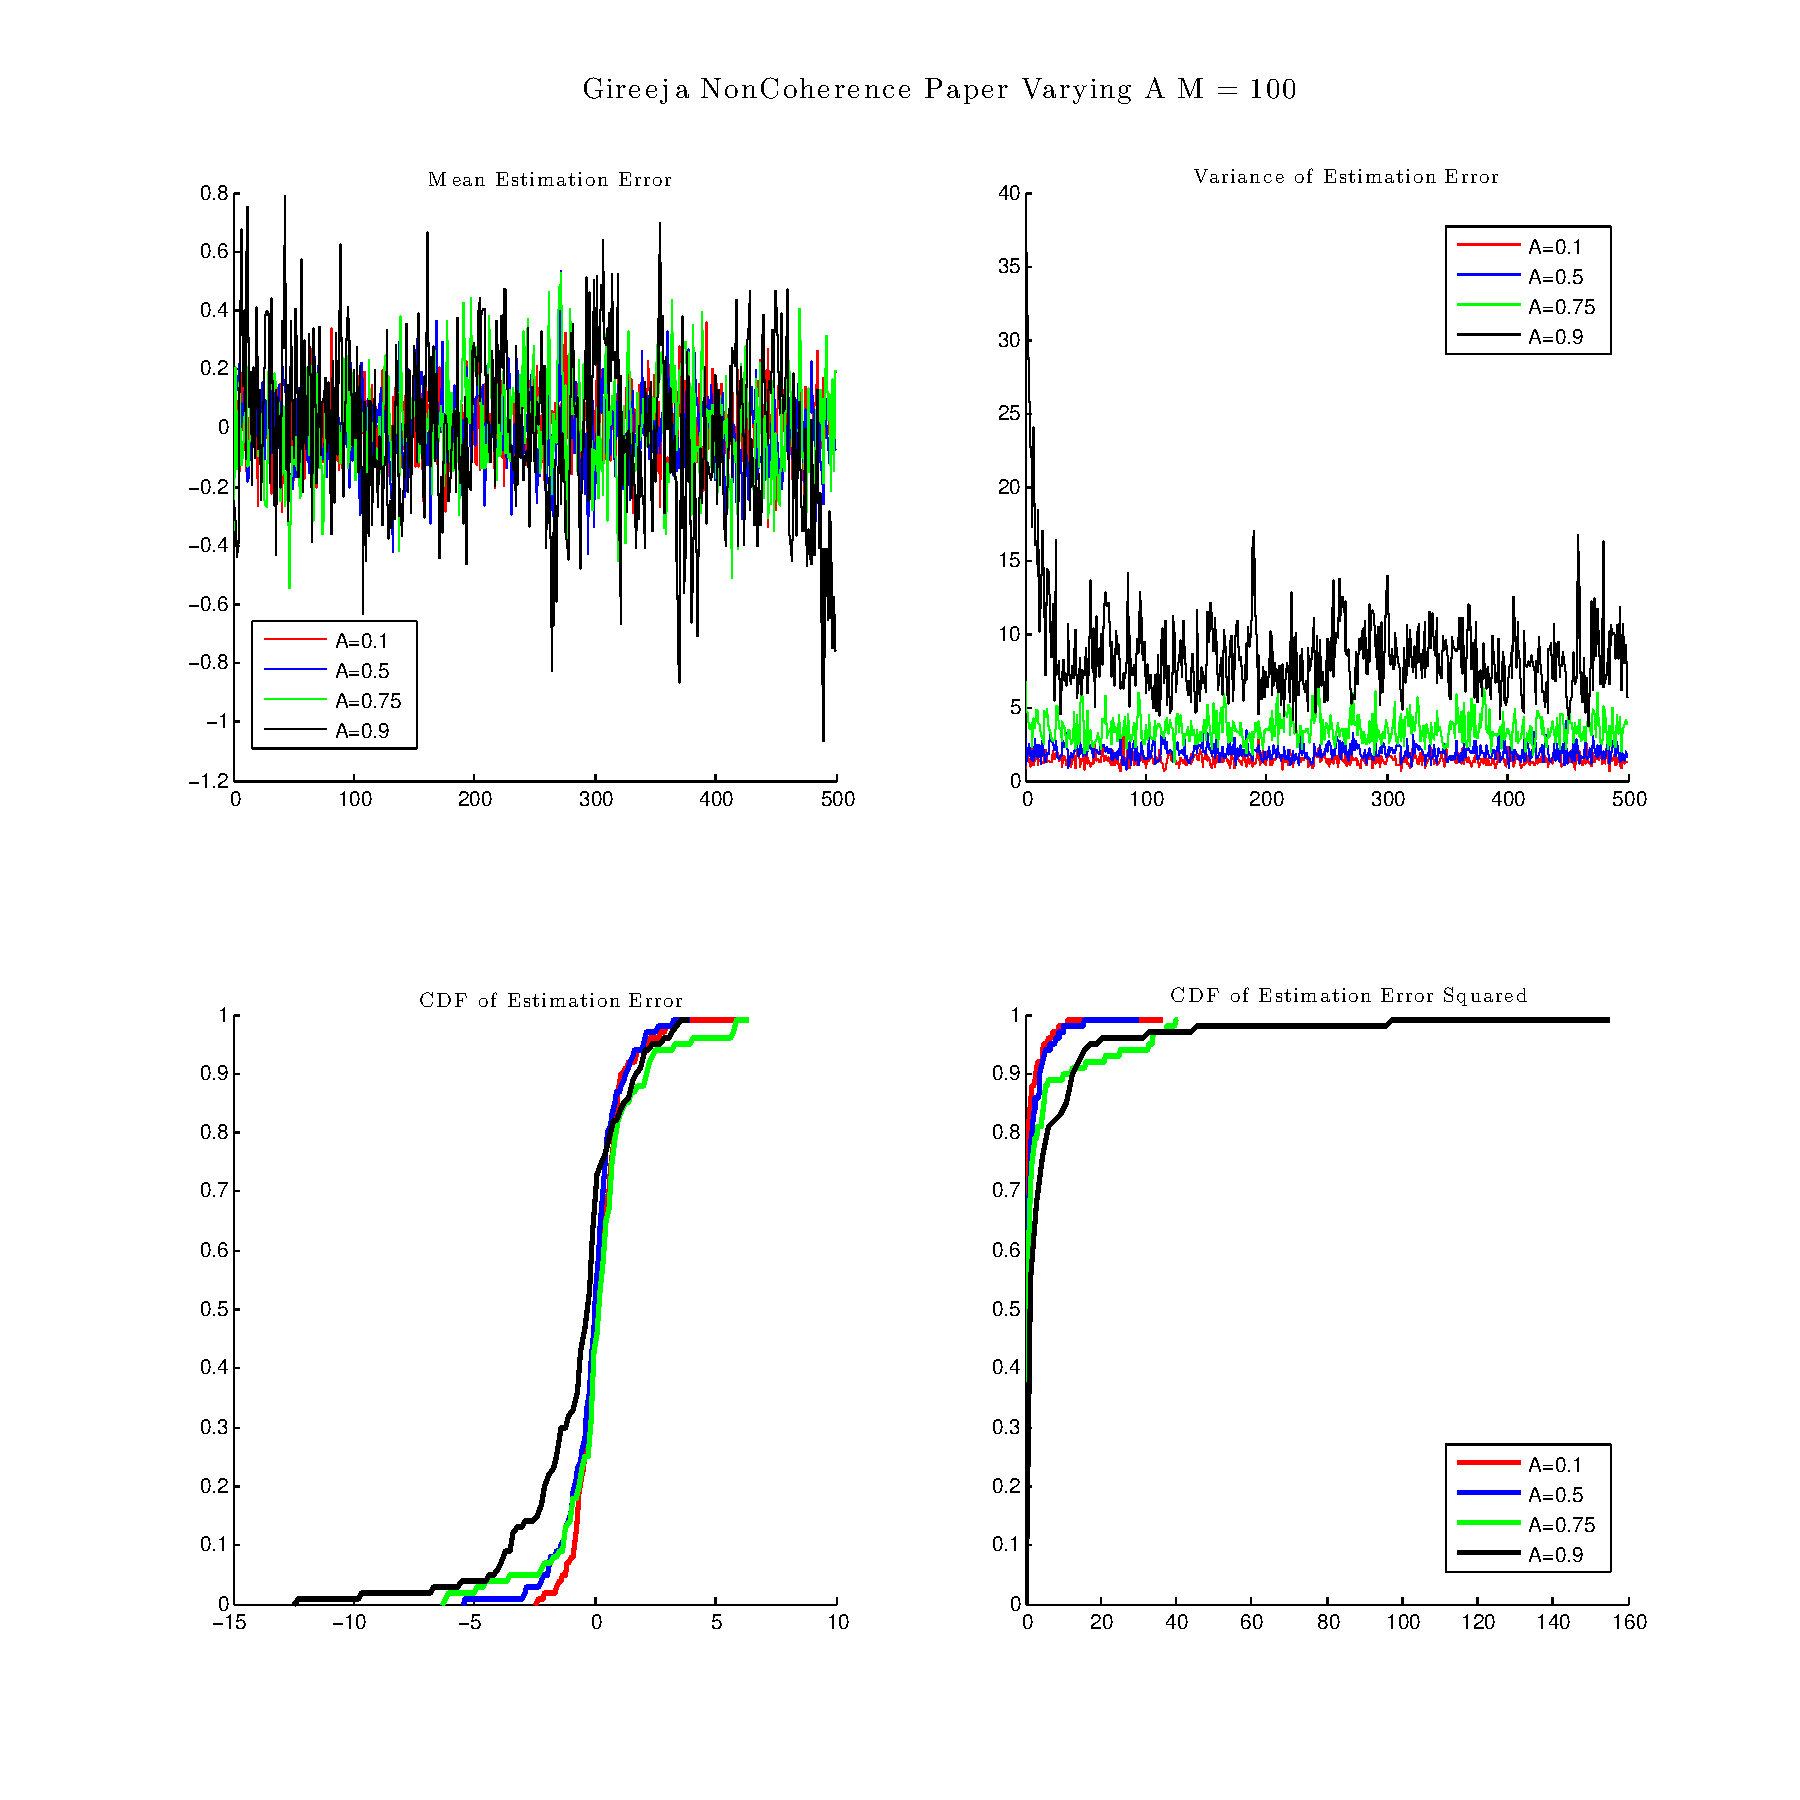
\includegraphics[width=\textwidth]{/Users/leahdickstein/Dropbox/R.edu/Sahai/140626/fig4_2}
\end{minipage}
\begin{minipage}[c]{0.5\textwidth}
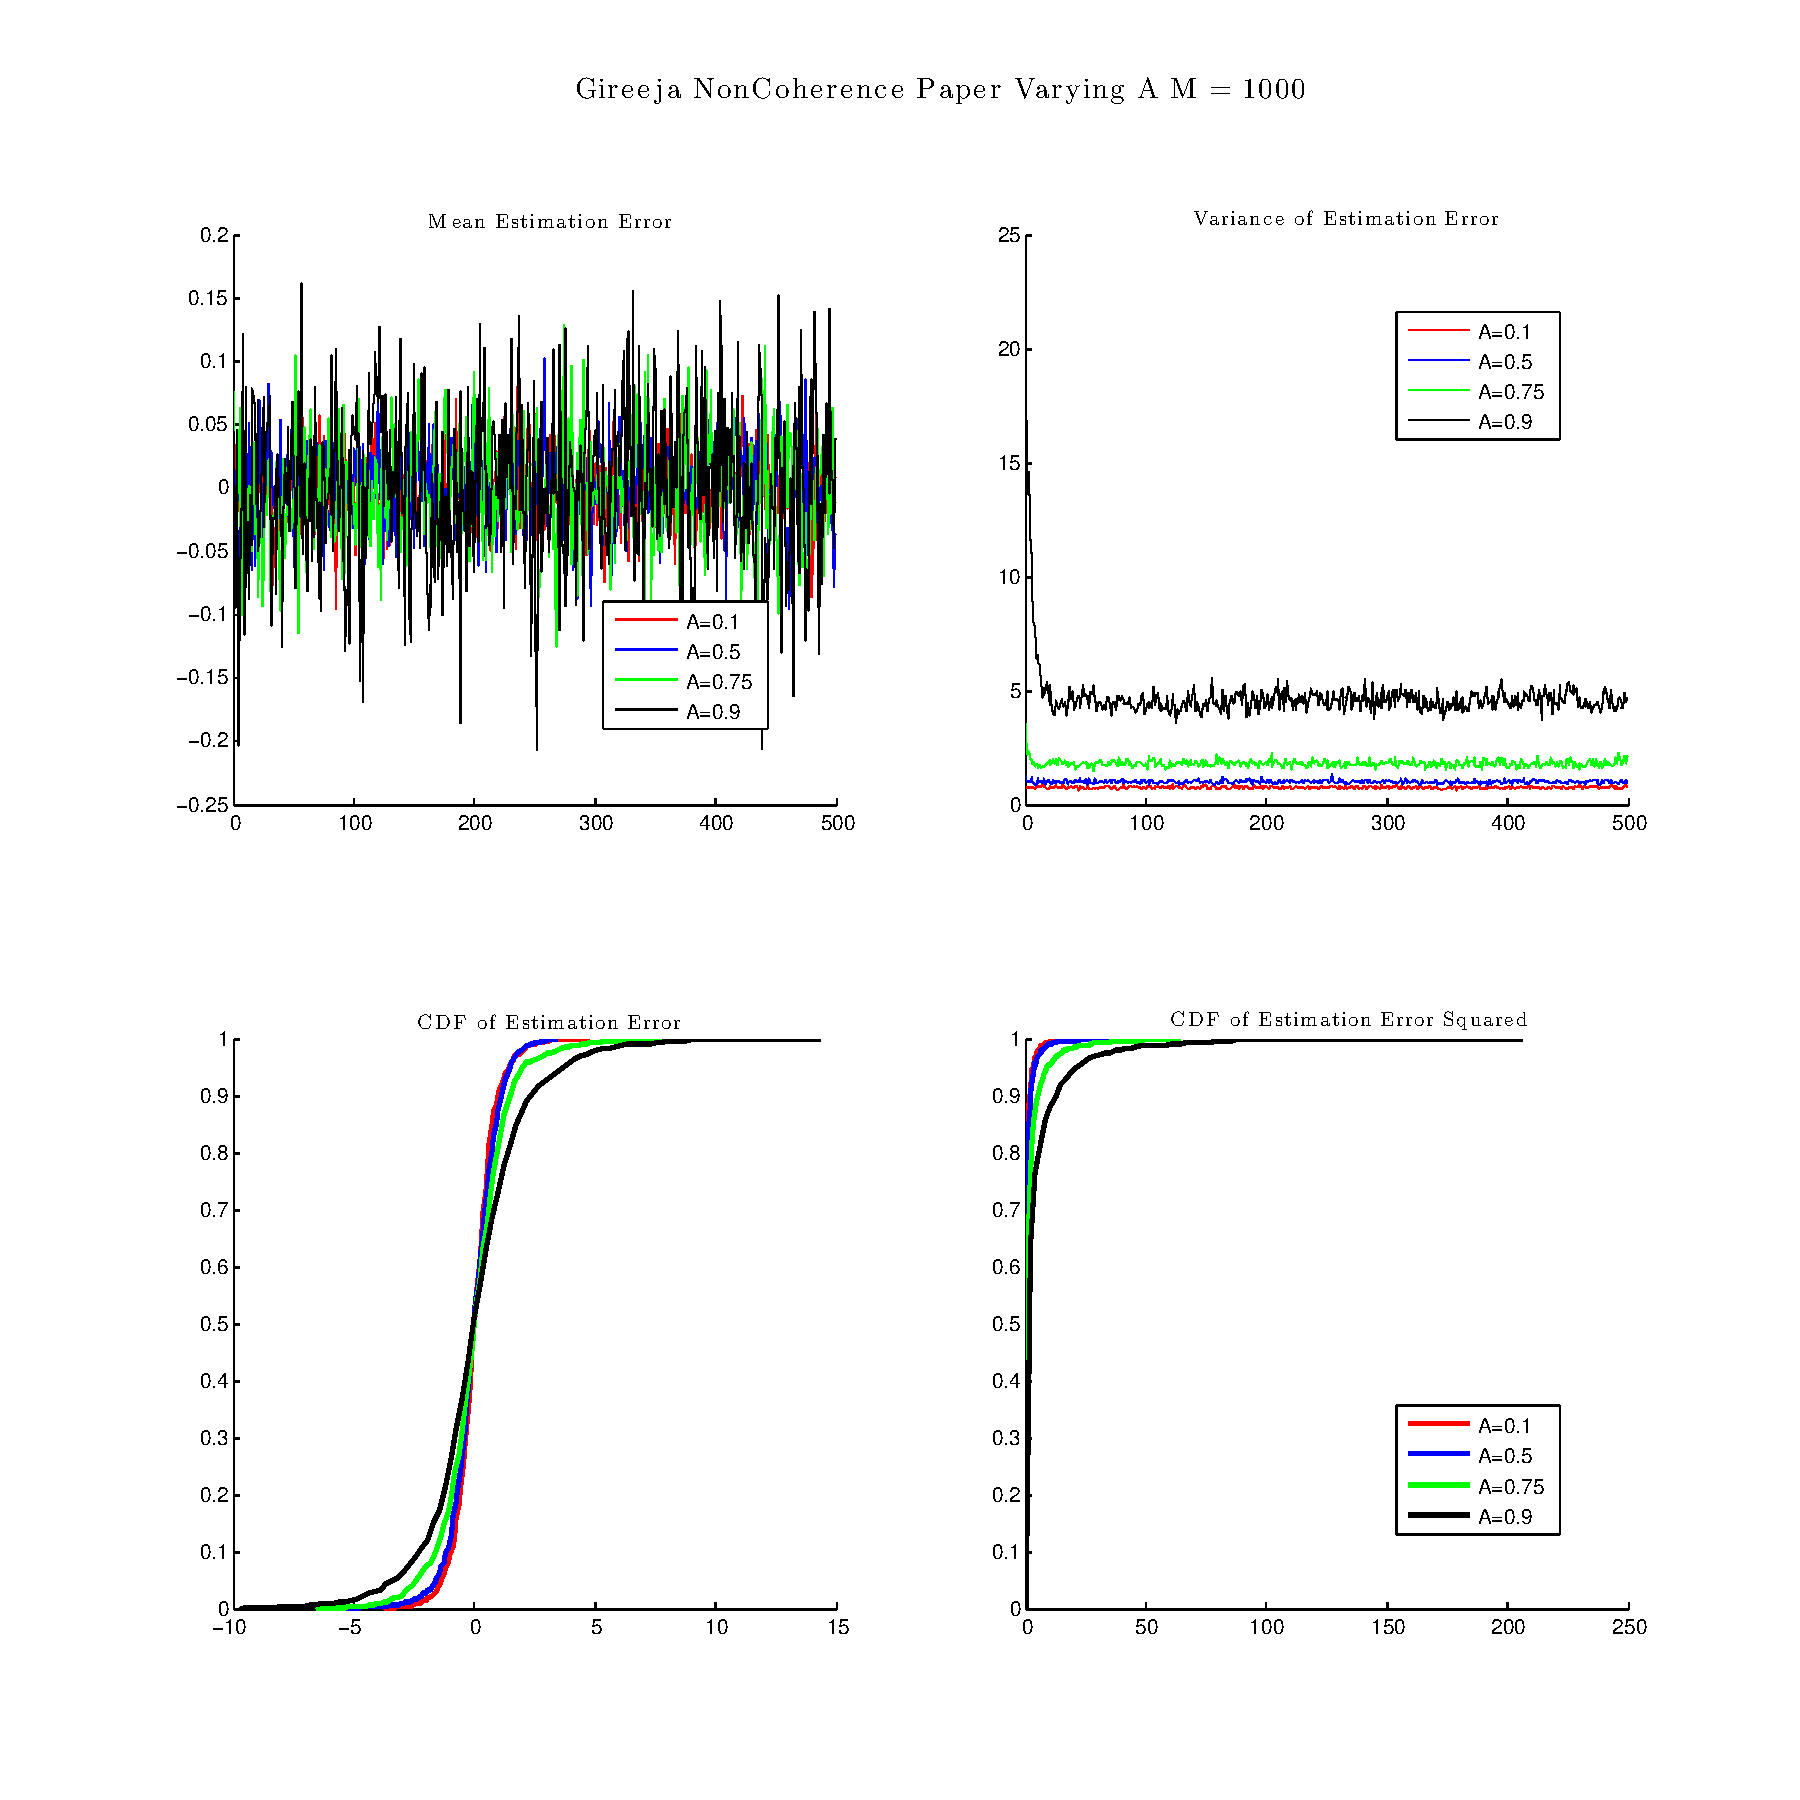
\includegraphics[width=\textwidth]{/Users/leahdickstein/Dropbox/R.edu/Sahai/140626/fig5_test_1}
\end{minipage}

\begin{minipage}[c]{0.5\textwidth}
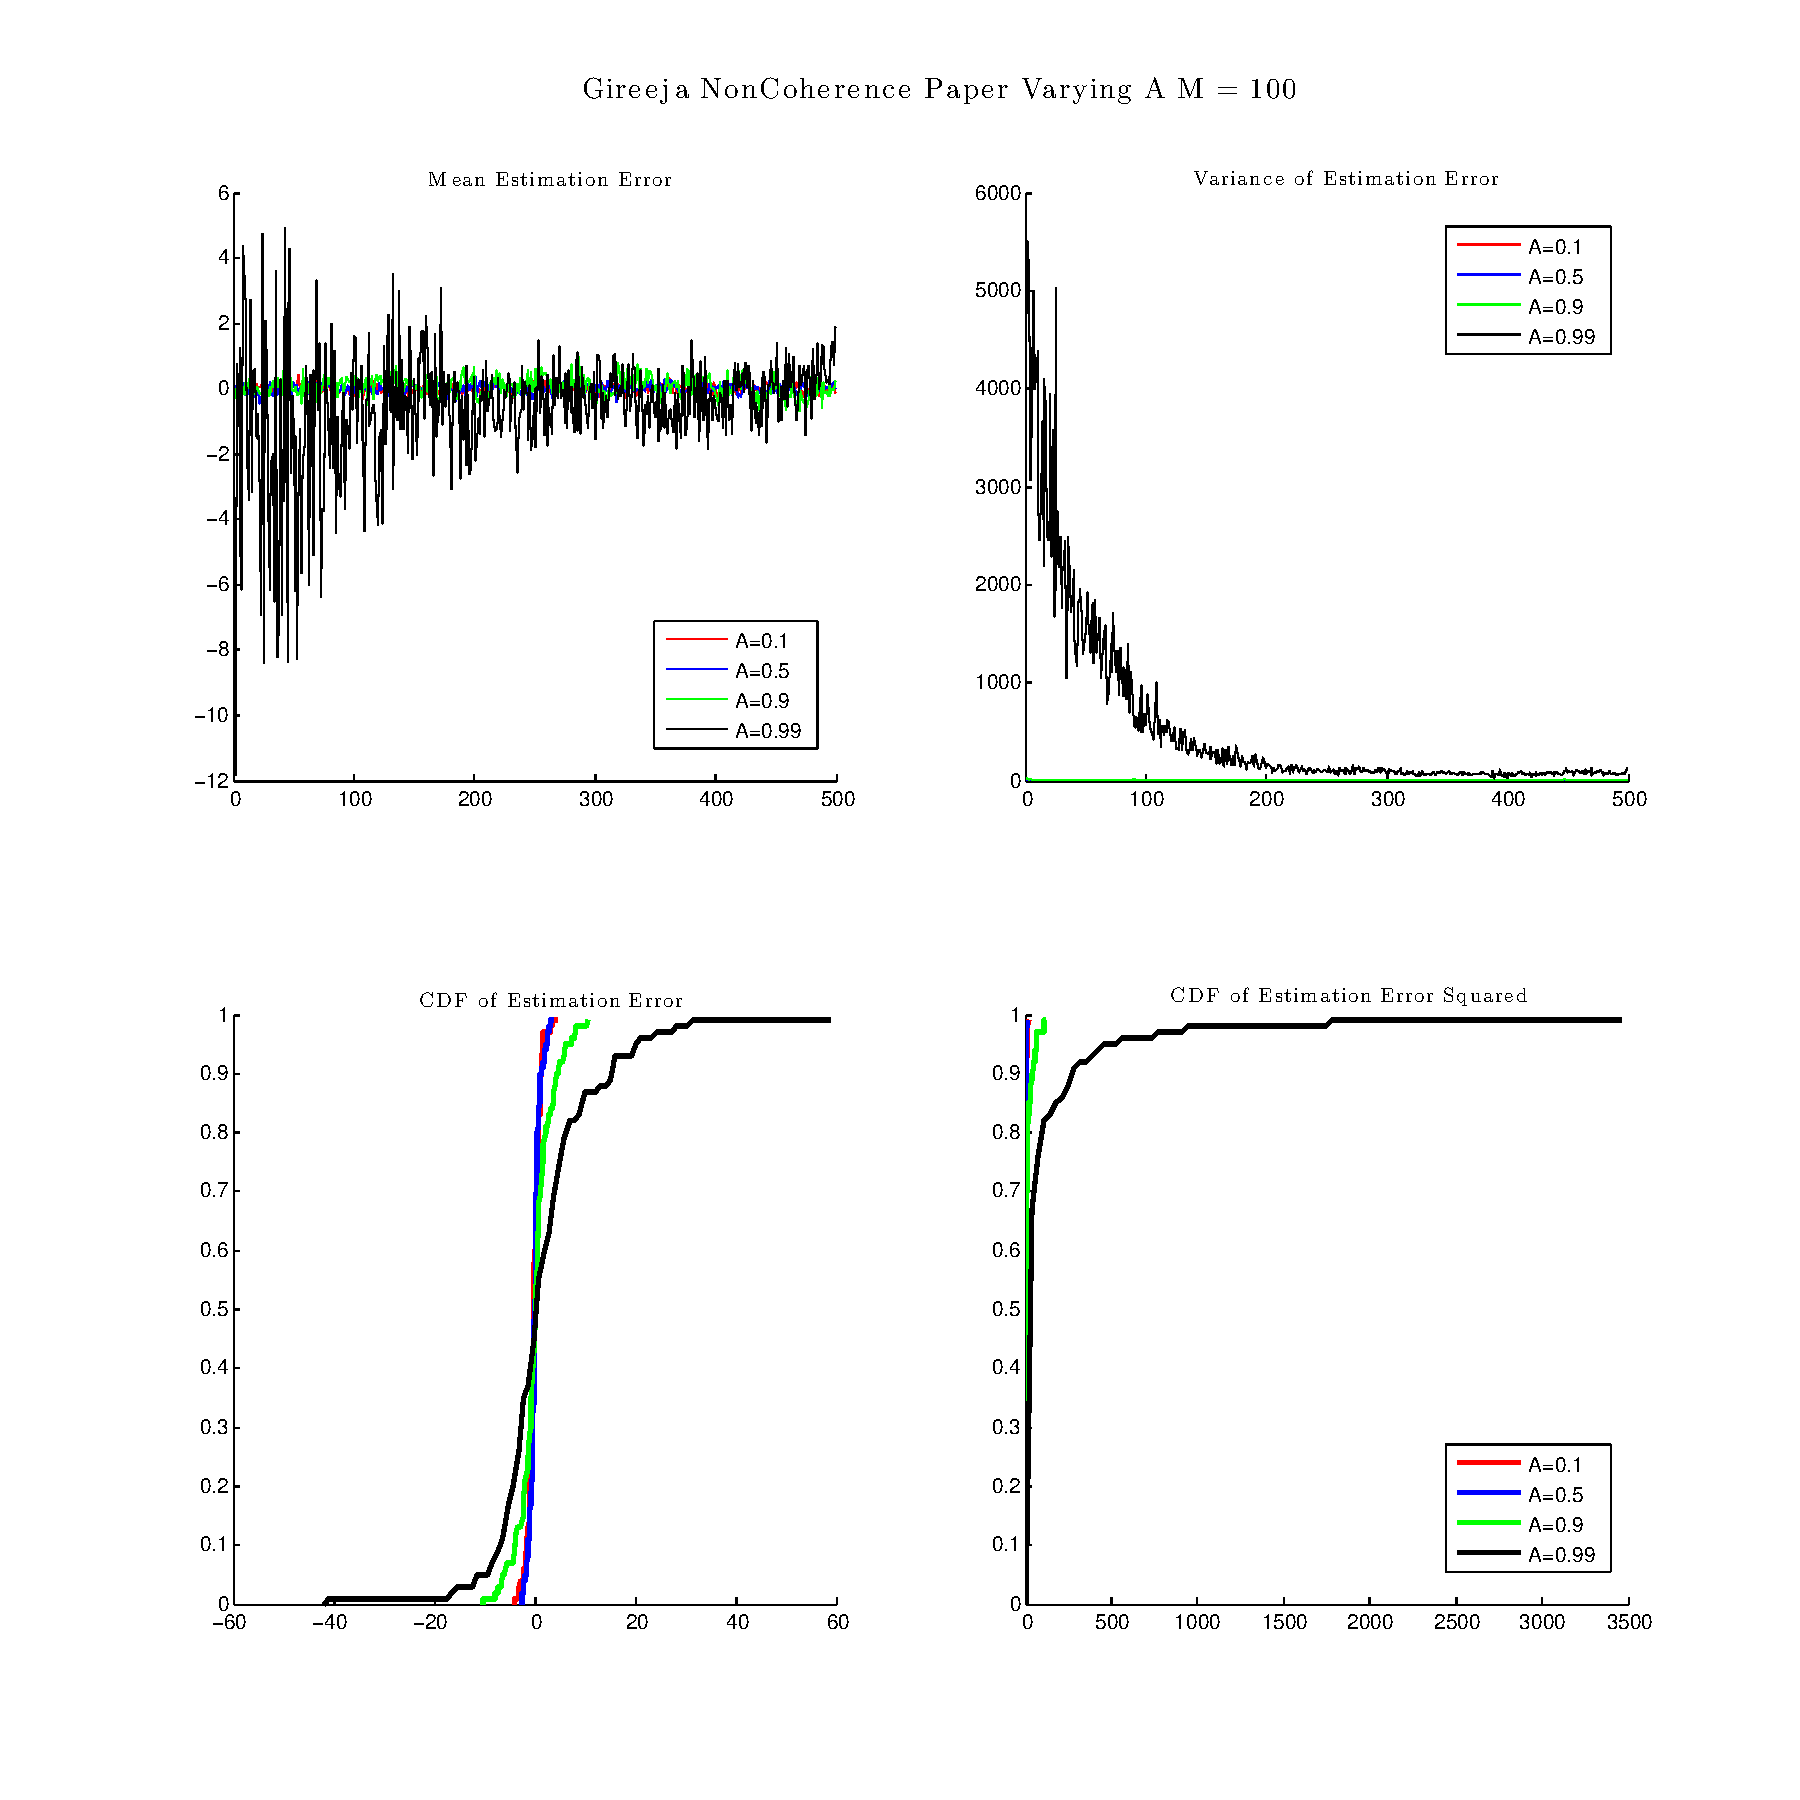
\includegraphics[width=\textwidth]{/Users/leahdickstein/Dropbox/R.edu/Sahai/140626/fig4_estimation}
\end{minipage}
\begin{minipage}[b]{0.5\textwidth}
These figures are the implementation of Gireeja's Non-Coherence paper for estimation, not control. The figures above show that A affects the final bounded value of the estimation error variance. The figure to the left shows why A must be $< 1$; when A is close to 1 it takes longer to converge towards its asymptotic estimation error variance, and when A $\geq 1$ the system will explode.
\end{minipage}

\subsection{NonCoherence Control: Gireeja}
\begin{minipage}[c]{0.5\textwidth}
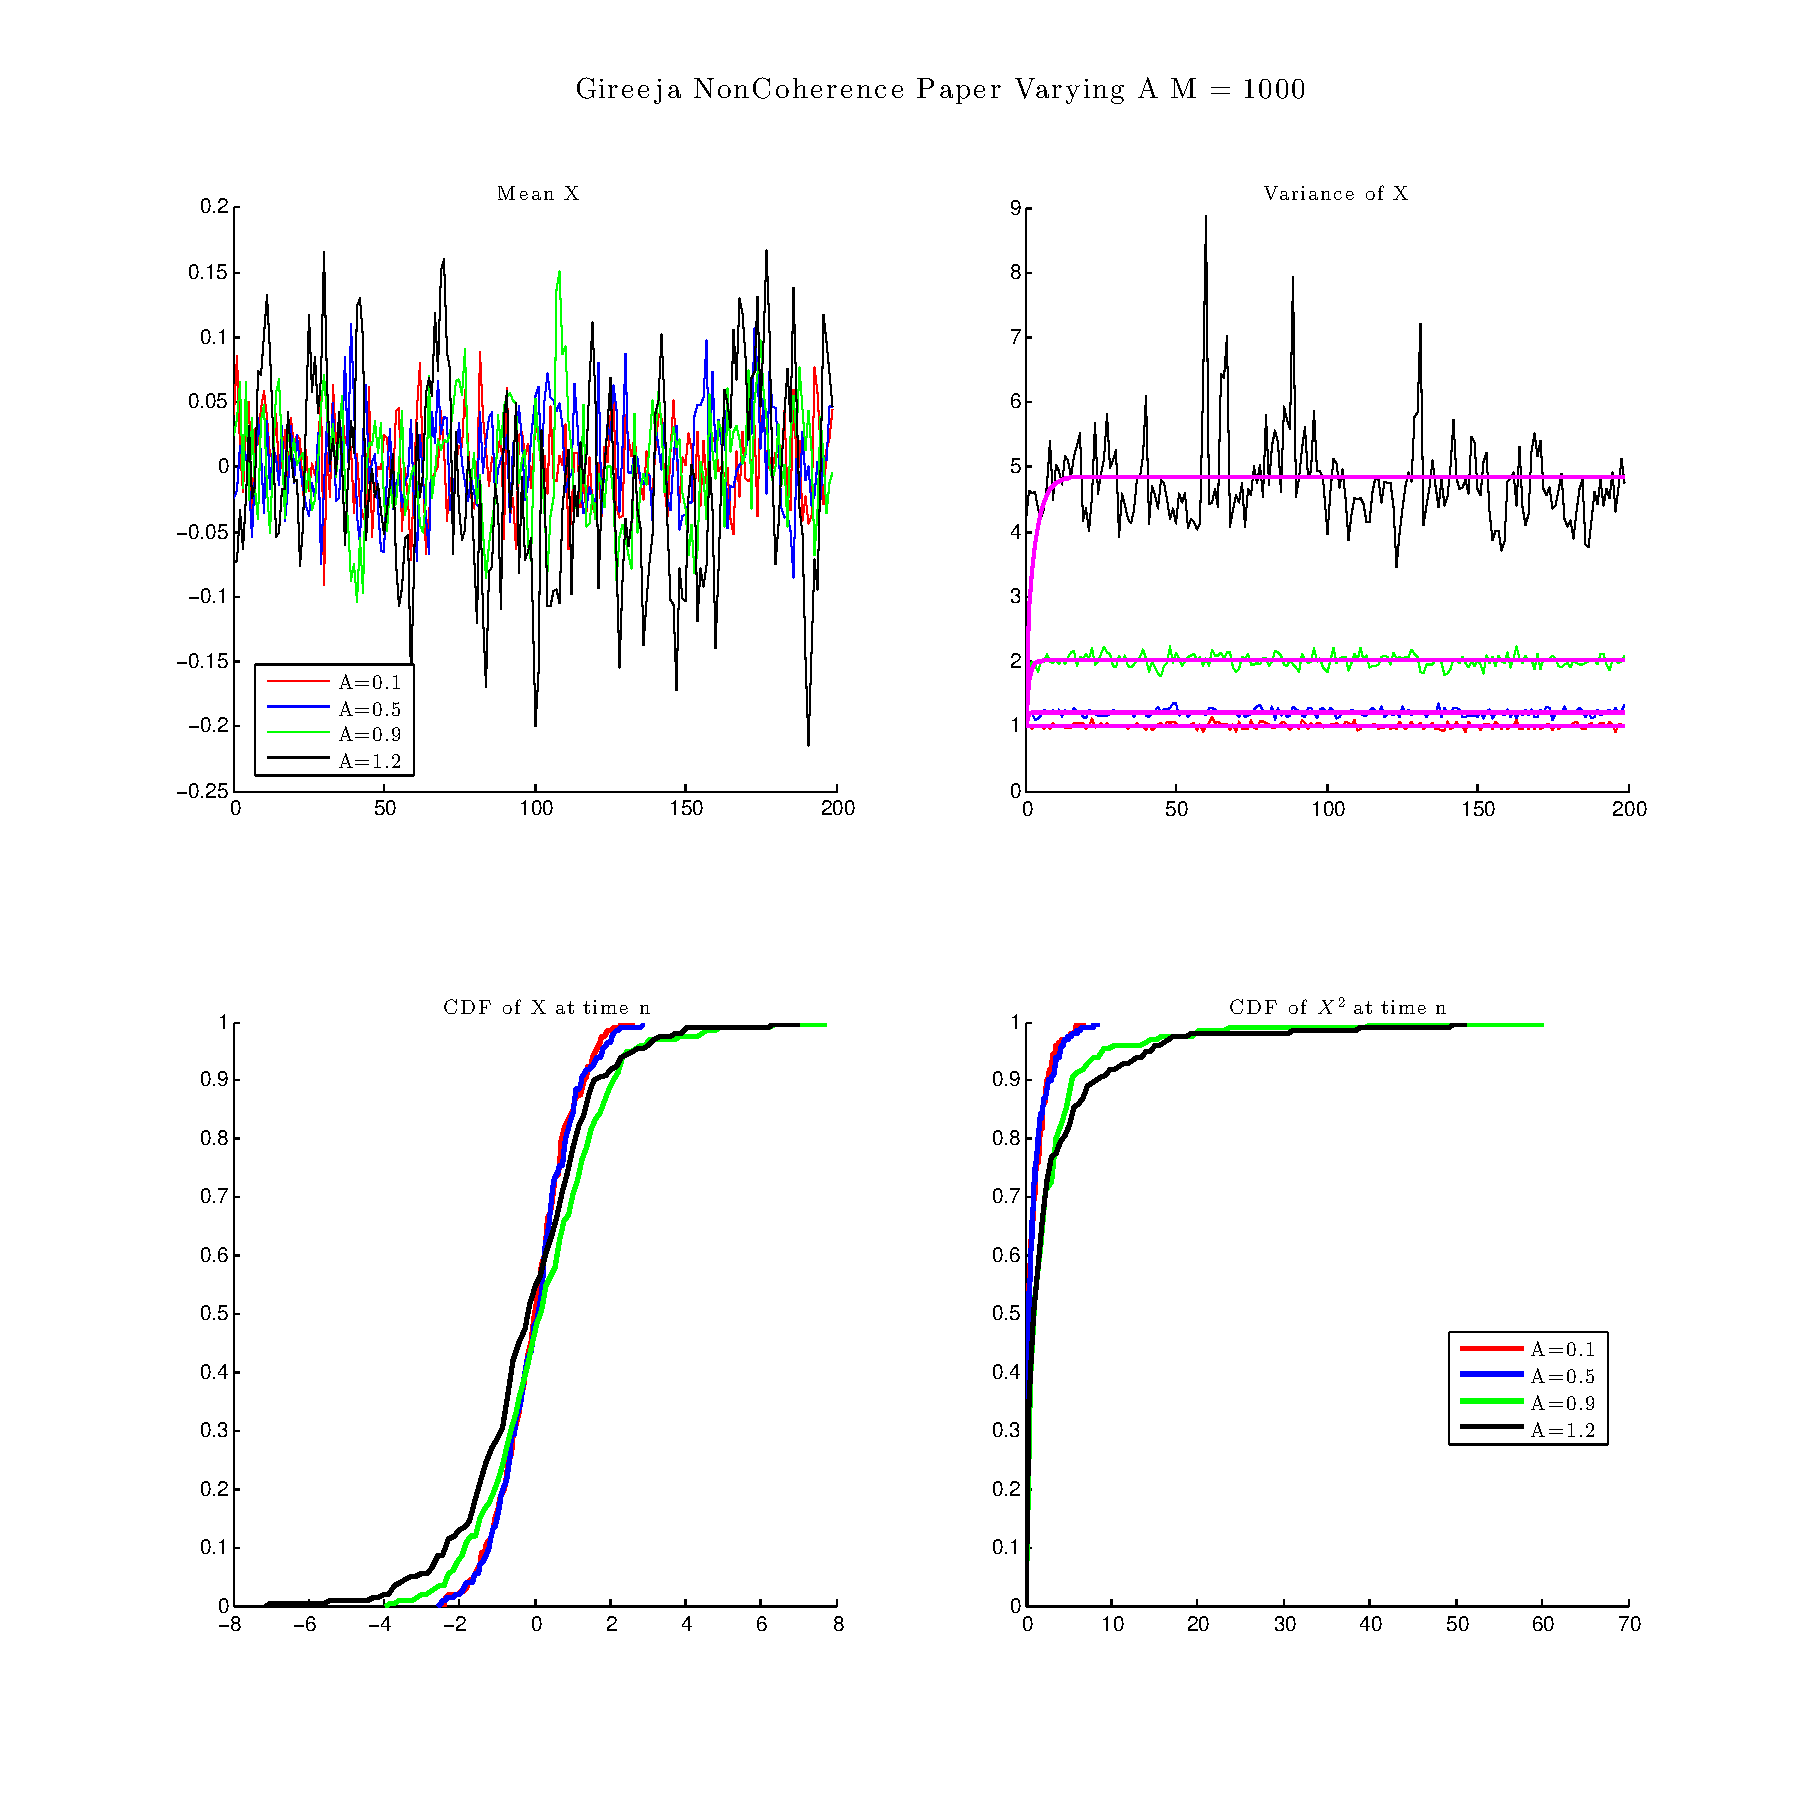
\includegraphics[width=\textwidth]{/Users/leahdickstein/Dropbox/R.edu/Sahai/140710/output0_1}
\end{minipage}
\begin{minipage}[c]{0.5\textwidth}
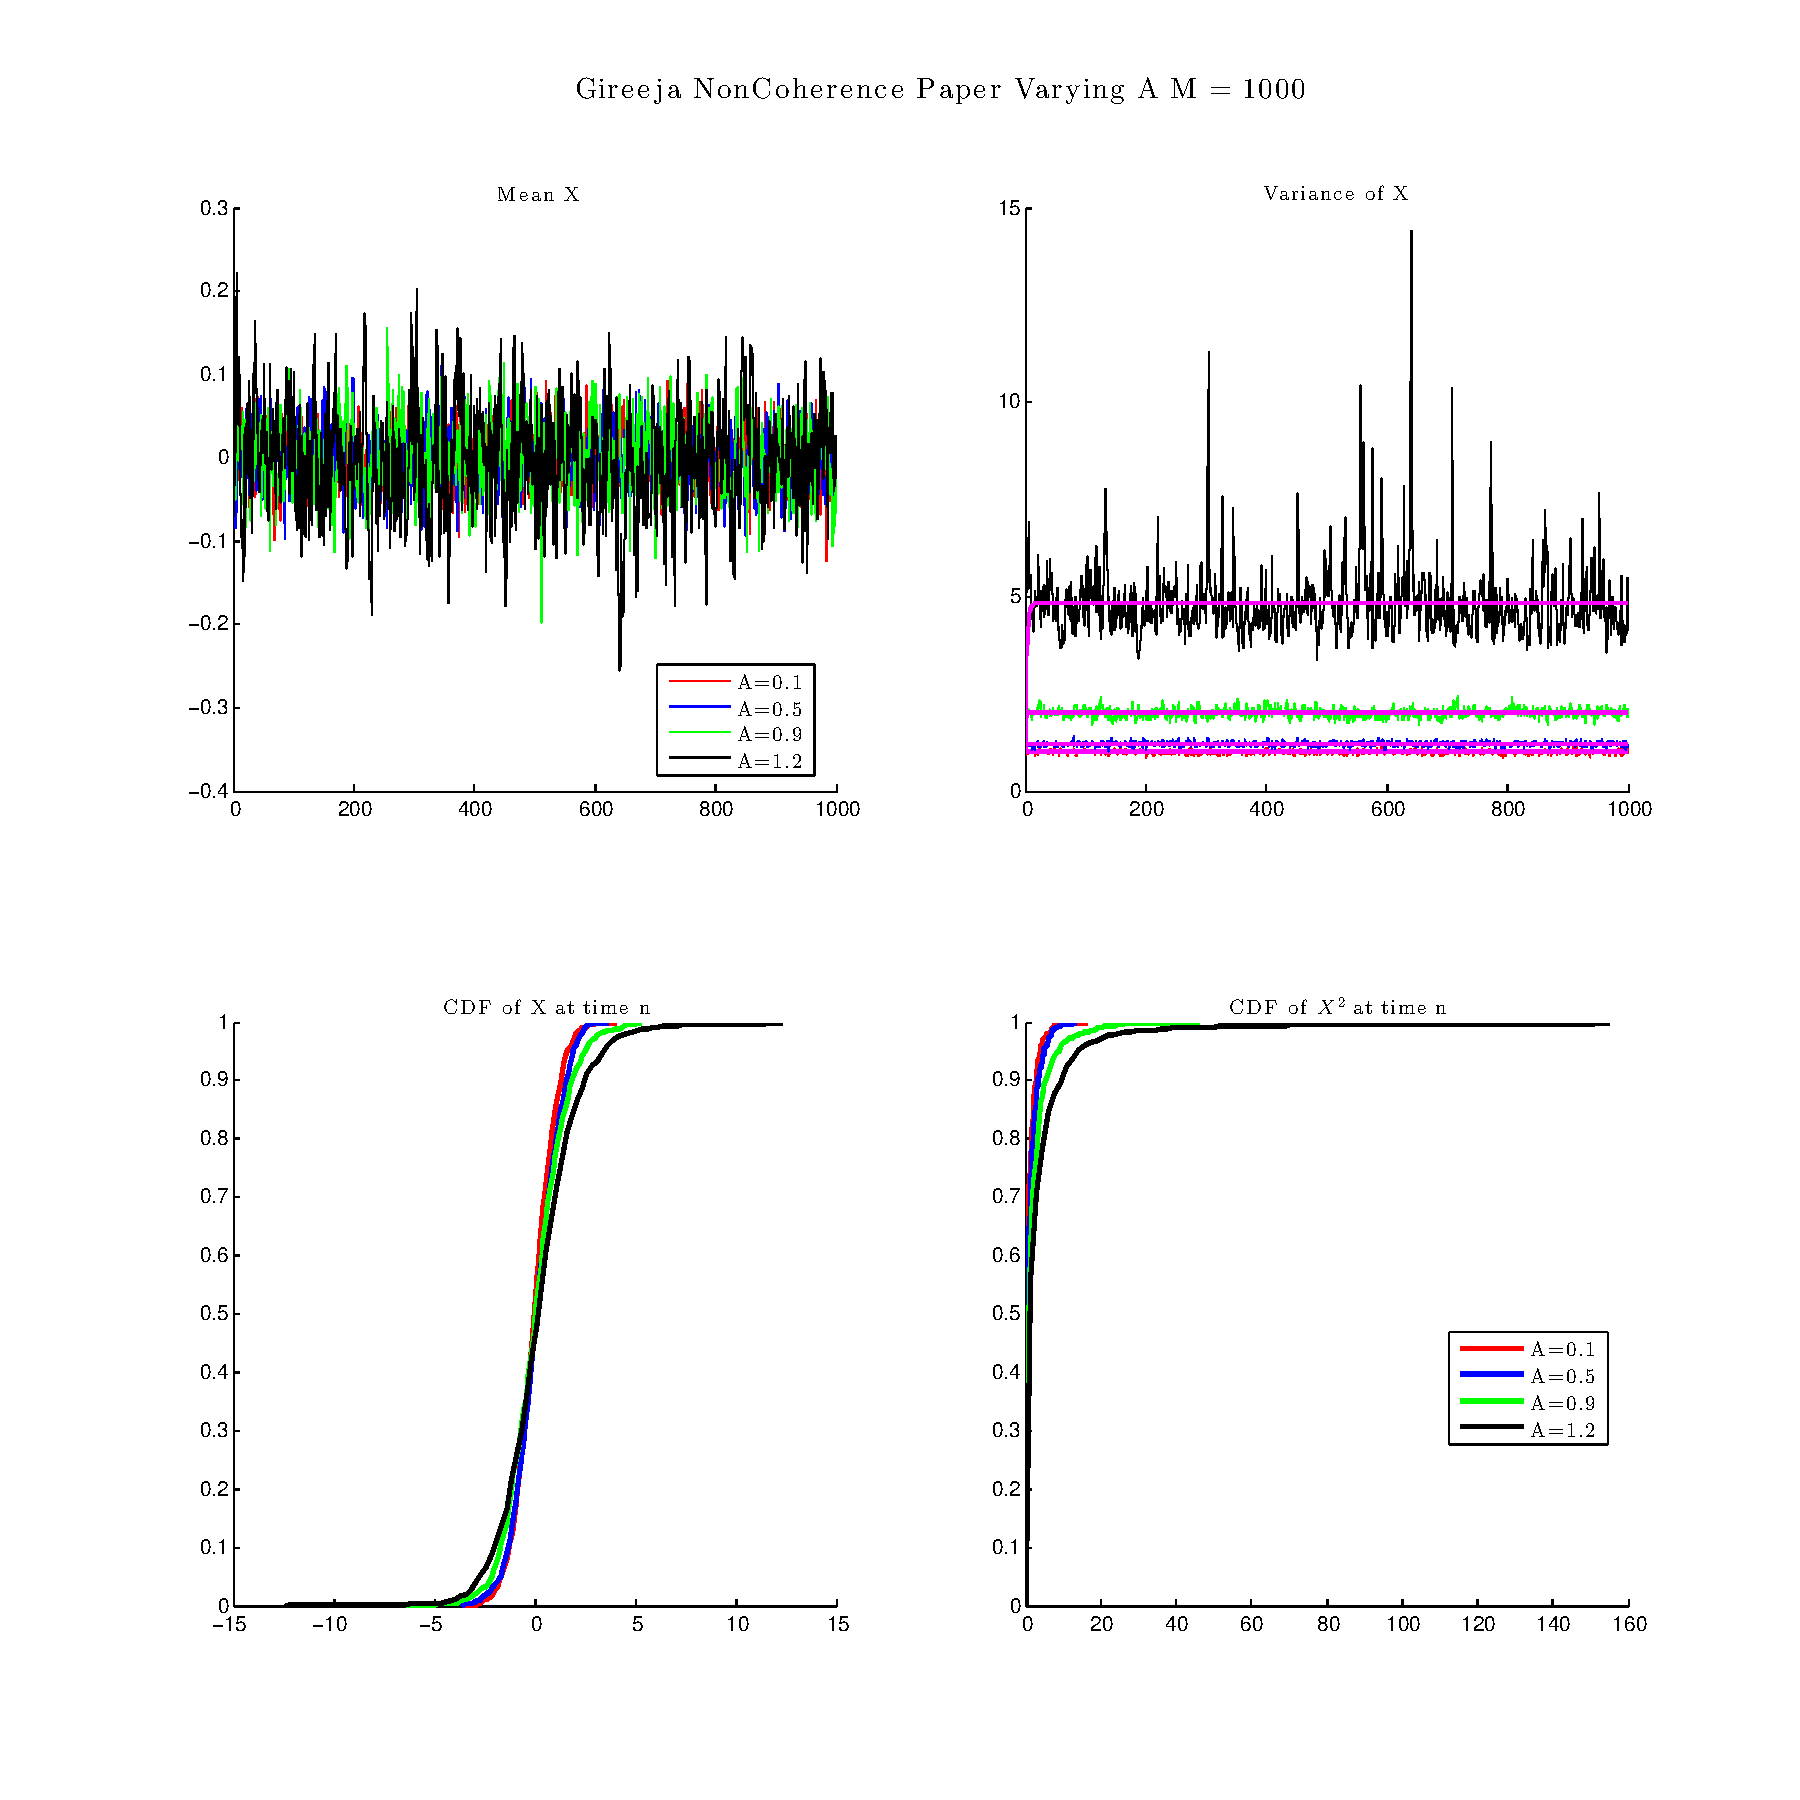
\includegraphics[width=\textwidth]{/Users/leahdickstein/Dropbox/R.edu/Sahai/140710/output0_2}
\end{minipage}

This figure is Gireeja's NonCoherence Paper Control System, and it shows the system is stabilized for varying levels of $A < 1.4$. Magenta represents the theoretical calculation for Var(X), and this figure reflects that that calculation is accurate. Over time, Var(X) quickly converges to $Var(X)^\infty$. In addition, the greater the A the higher the state variance, and this can be calculated.

\subsection{Varying A, NonCoherence Control, Gireeja}
\begin{minipage}[c]{0.5\textwidth}
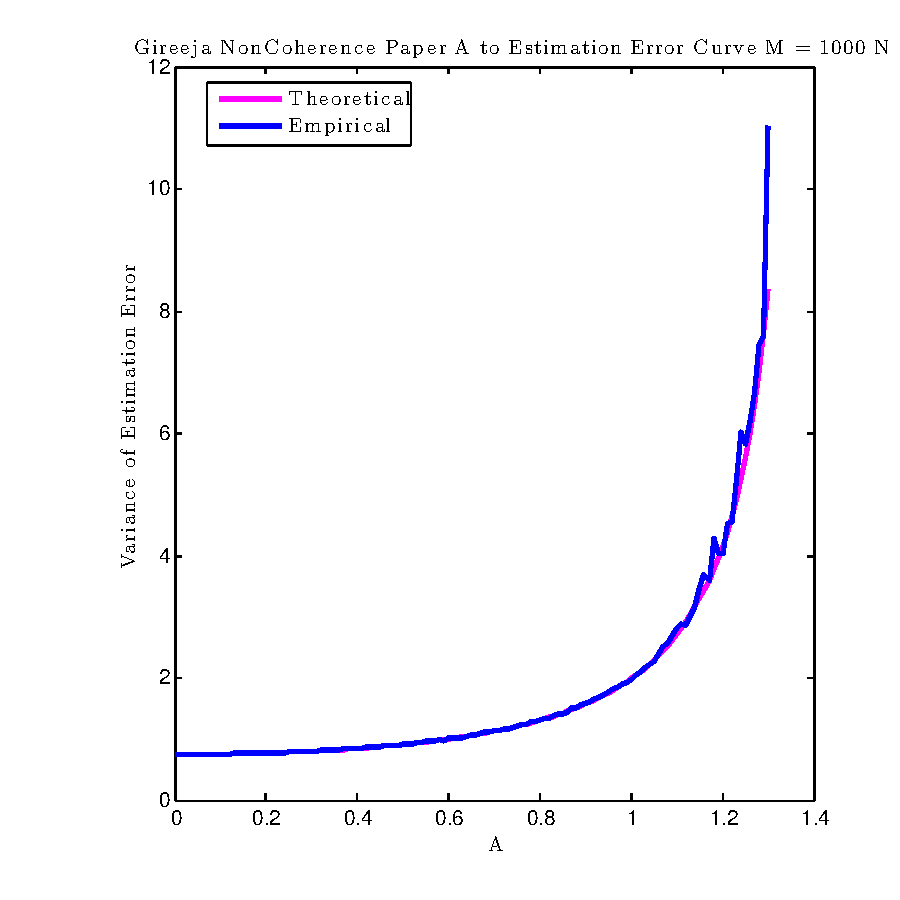
\includegraphics[width=\textwidth]{/Users/leahdickstein/Dropbox/R.edu/Sahai/140706/output1}
\end{minipage}
\begin{minipage}[b]{0.5\textwidth}
\textcolor{red}{THIS NEEDS TO BE UPDATED!!} In this figure, blue represents the asymptotic empirical variance for levels of A 0:0.01:1.3, while magenta represents the asymptotic theoretical variance. These values are mean(mean()), or averaged over both trials and timesteps. The curve appears roughly exponential, or at the very least when $A > 1$ the curve rises sharply. Based on Gireeja's paper, for these values the curve should asymptote at $\sqrt{2} = 1.414$, which is reflected in the curve. Since this curve was generated over n = 250 timesteps and M = 1000 trials, the spikes in the blue curve should \textit{not} be attributed to randomness. \textcolor{red}{Multiple runs could confirm whether those spikes are significant or not.}
\end{minipage}

\subsection{Rajasekaran vs Schenato: Prediction vs Estimation}
\begin{minipage}[c]{0.5\textwidth}
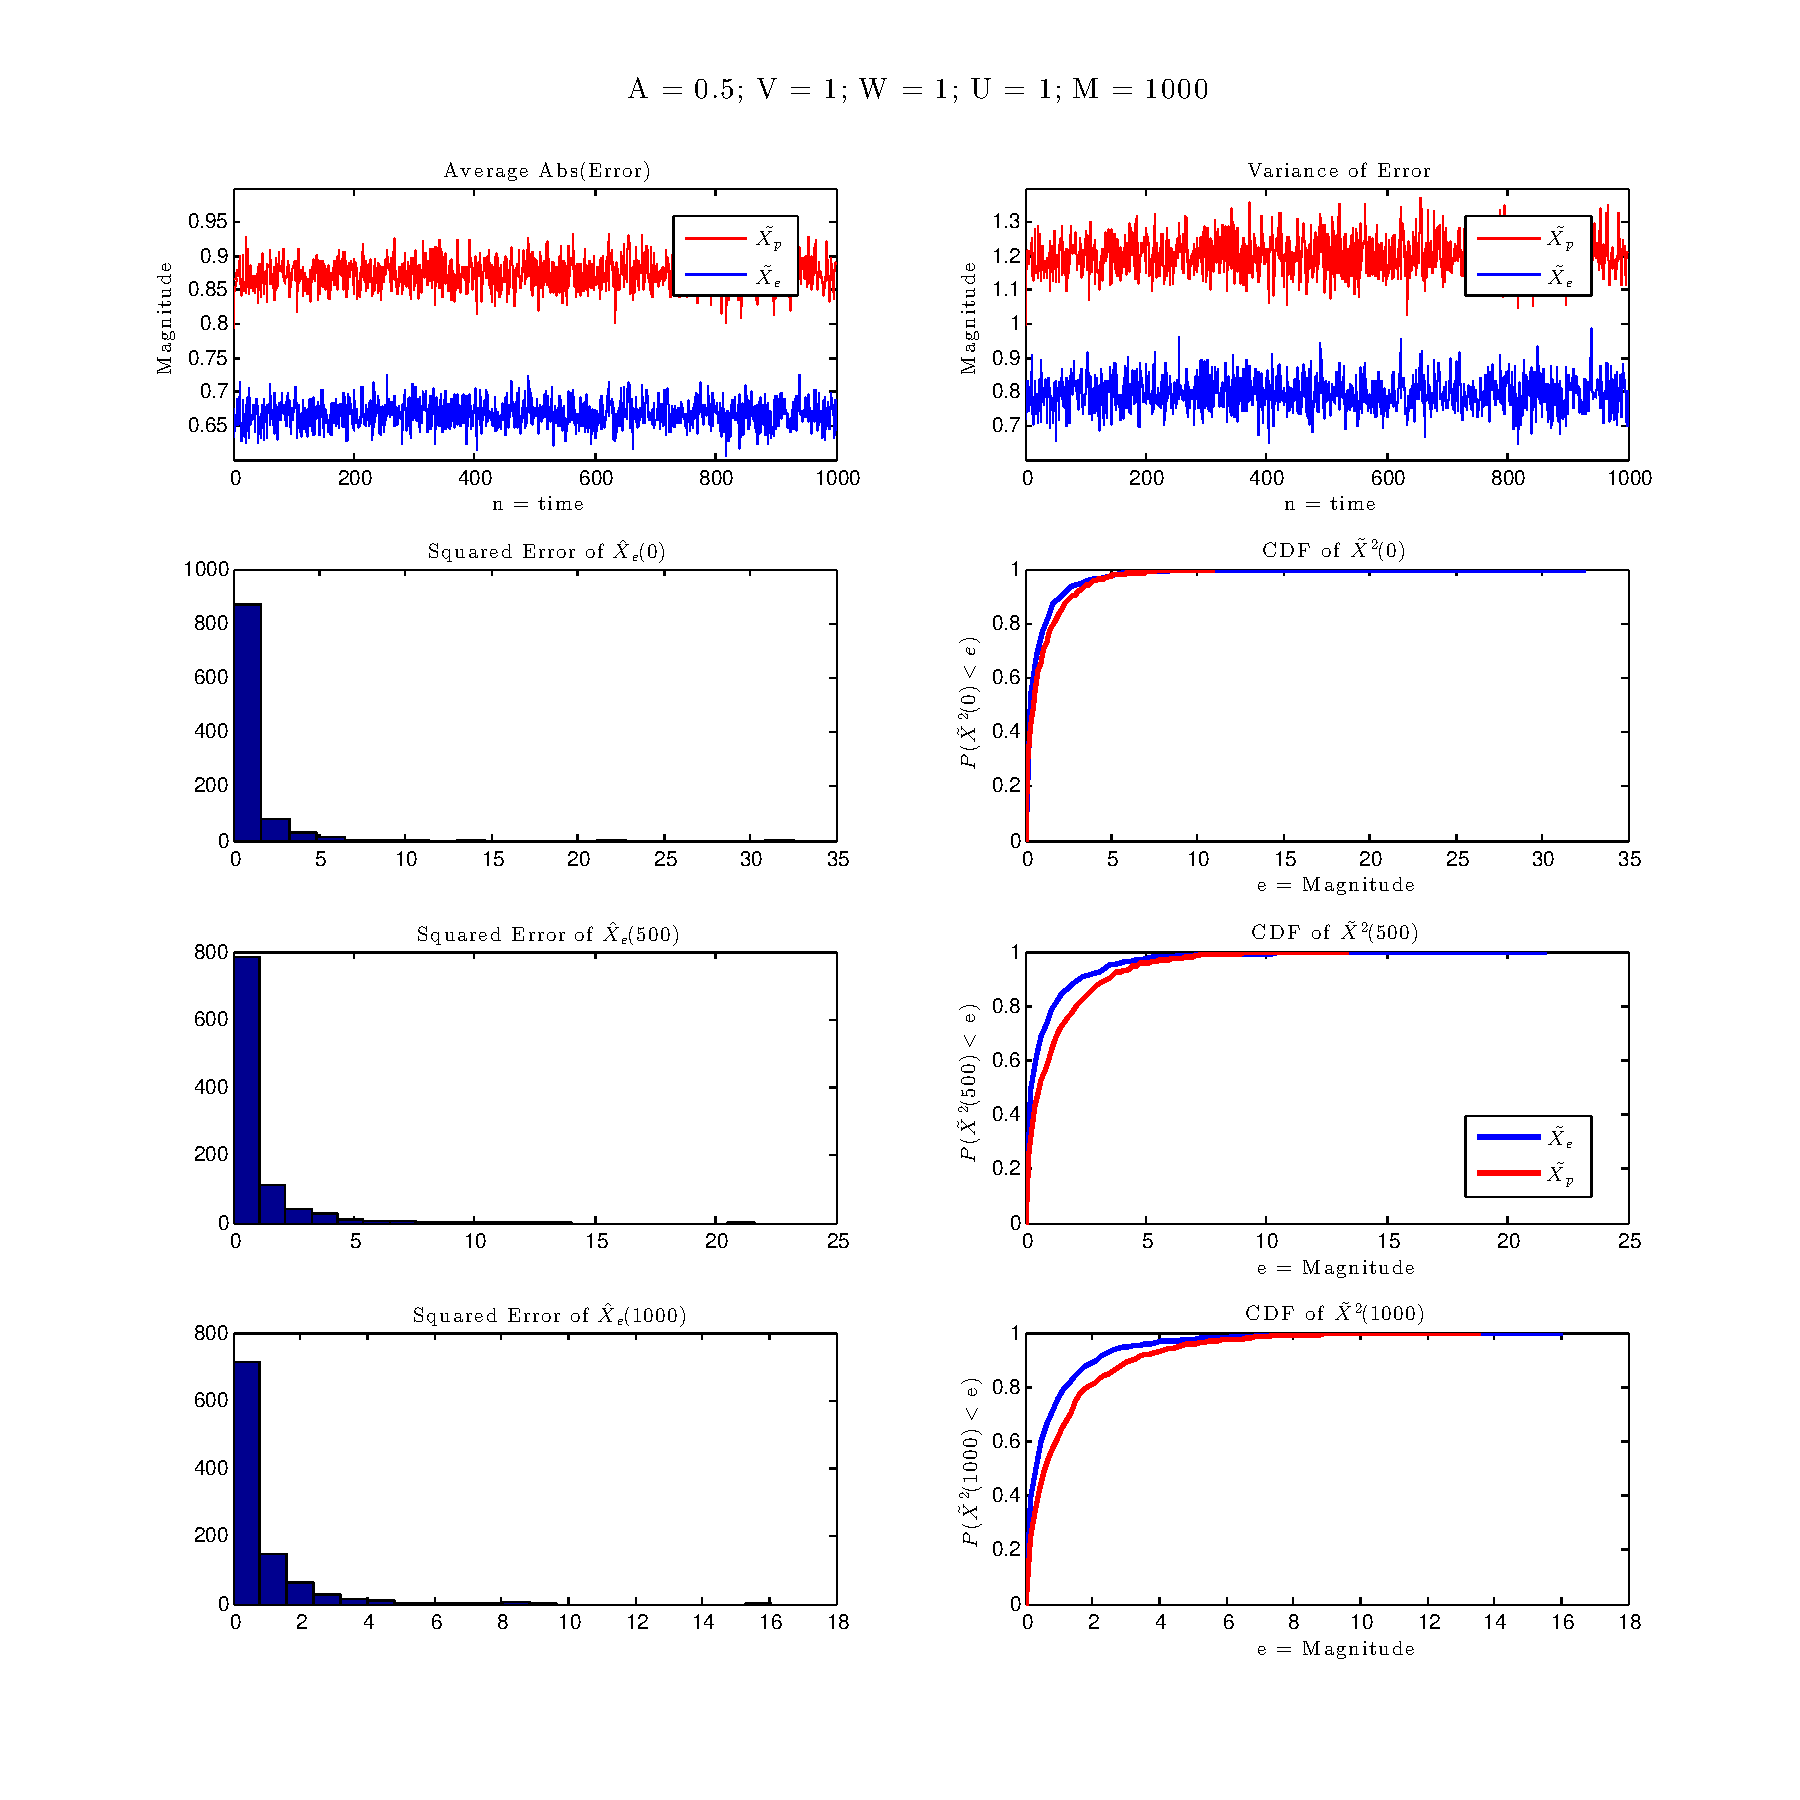
\includegraphics[width=\textwidth]{/Users/leahdickstein/Dropbox/R.edu/Sahai/140710/raj_a05_p1}
\end{minipage}
\begin{minipage}[c]{0.5\textwidth}
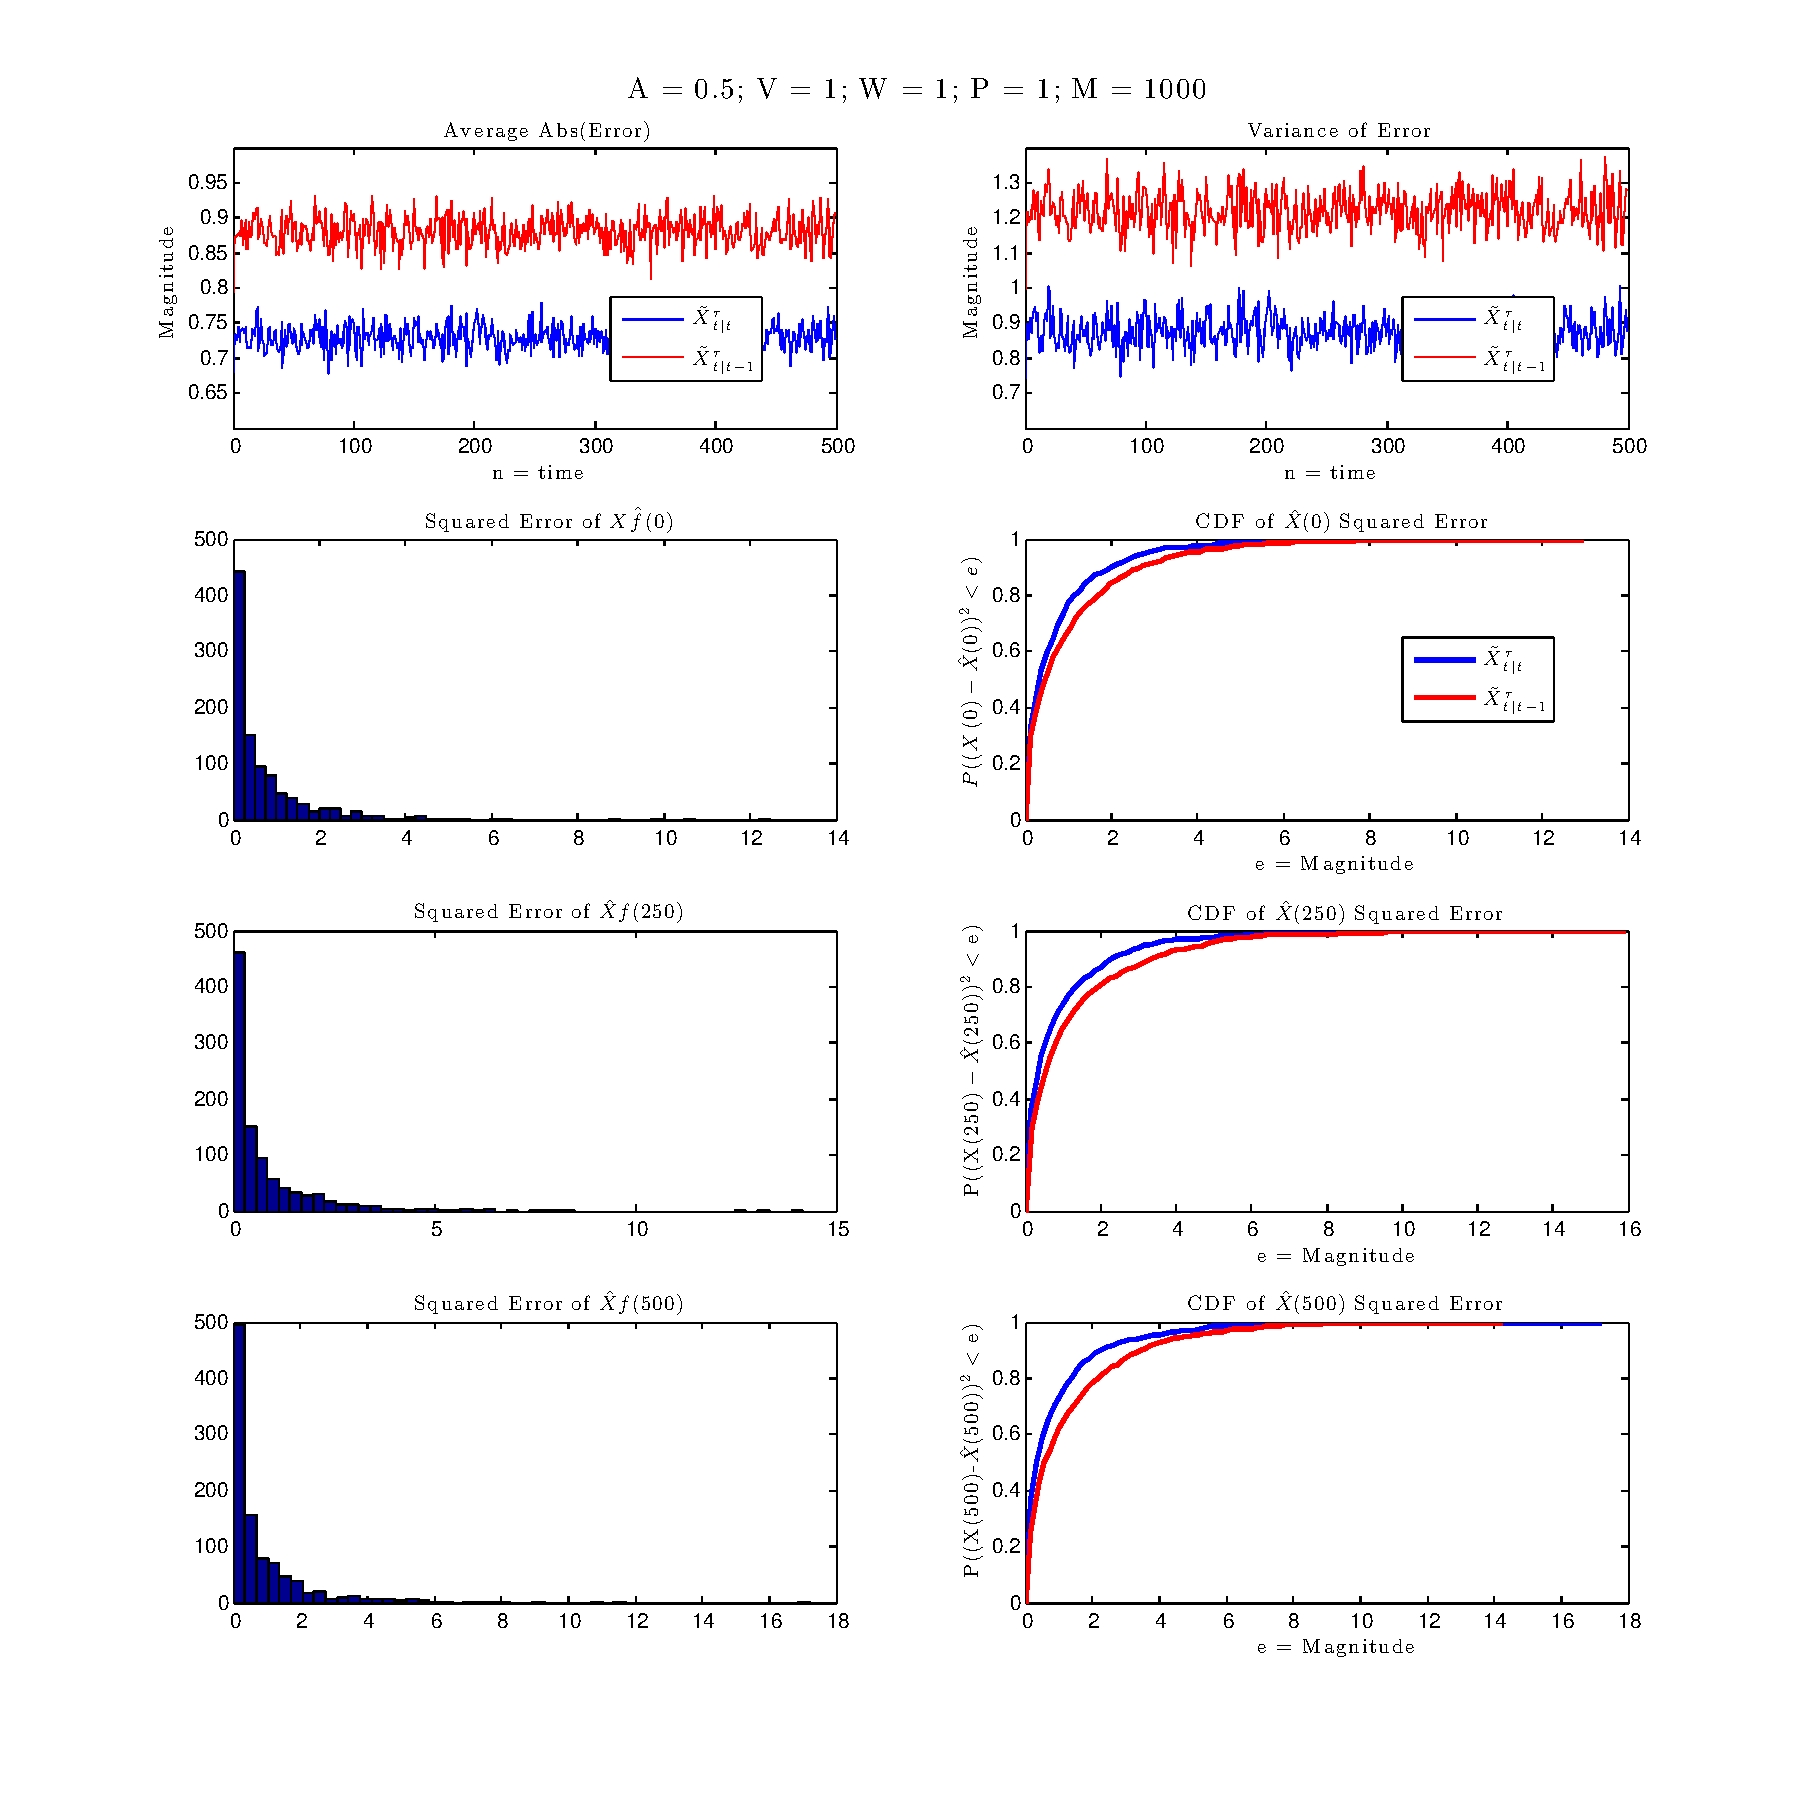
\includegraphics[width=\textwidth]{/Users/leahdickstein/Dropbox/R.edu/Sahai/140710/schenato_a05_p1}
\end{minipage}

\begin{minipage}[c]{0.5\textwidth}
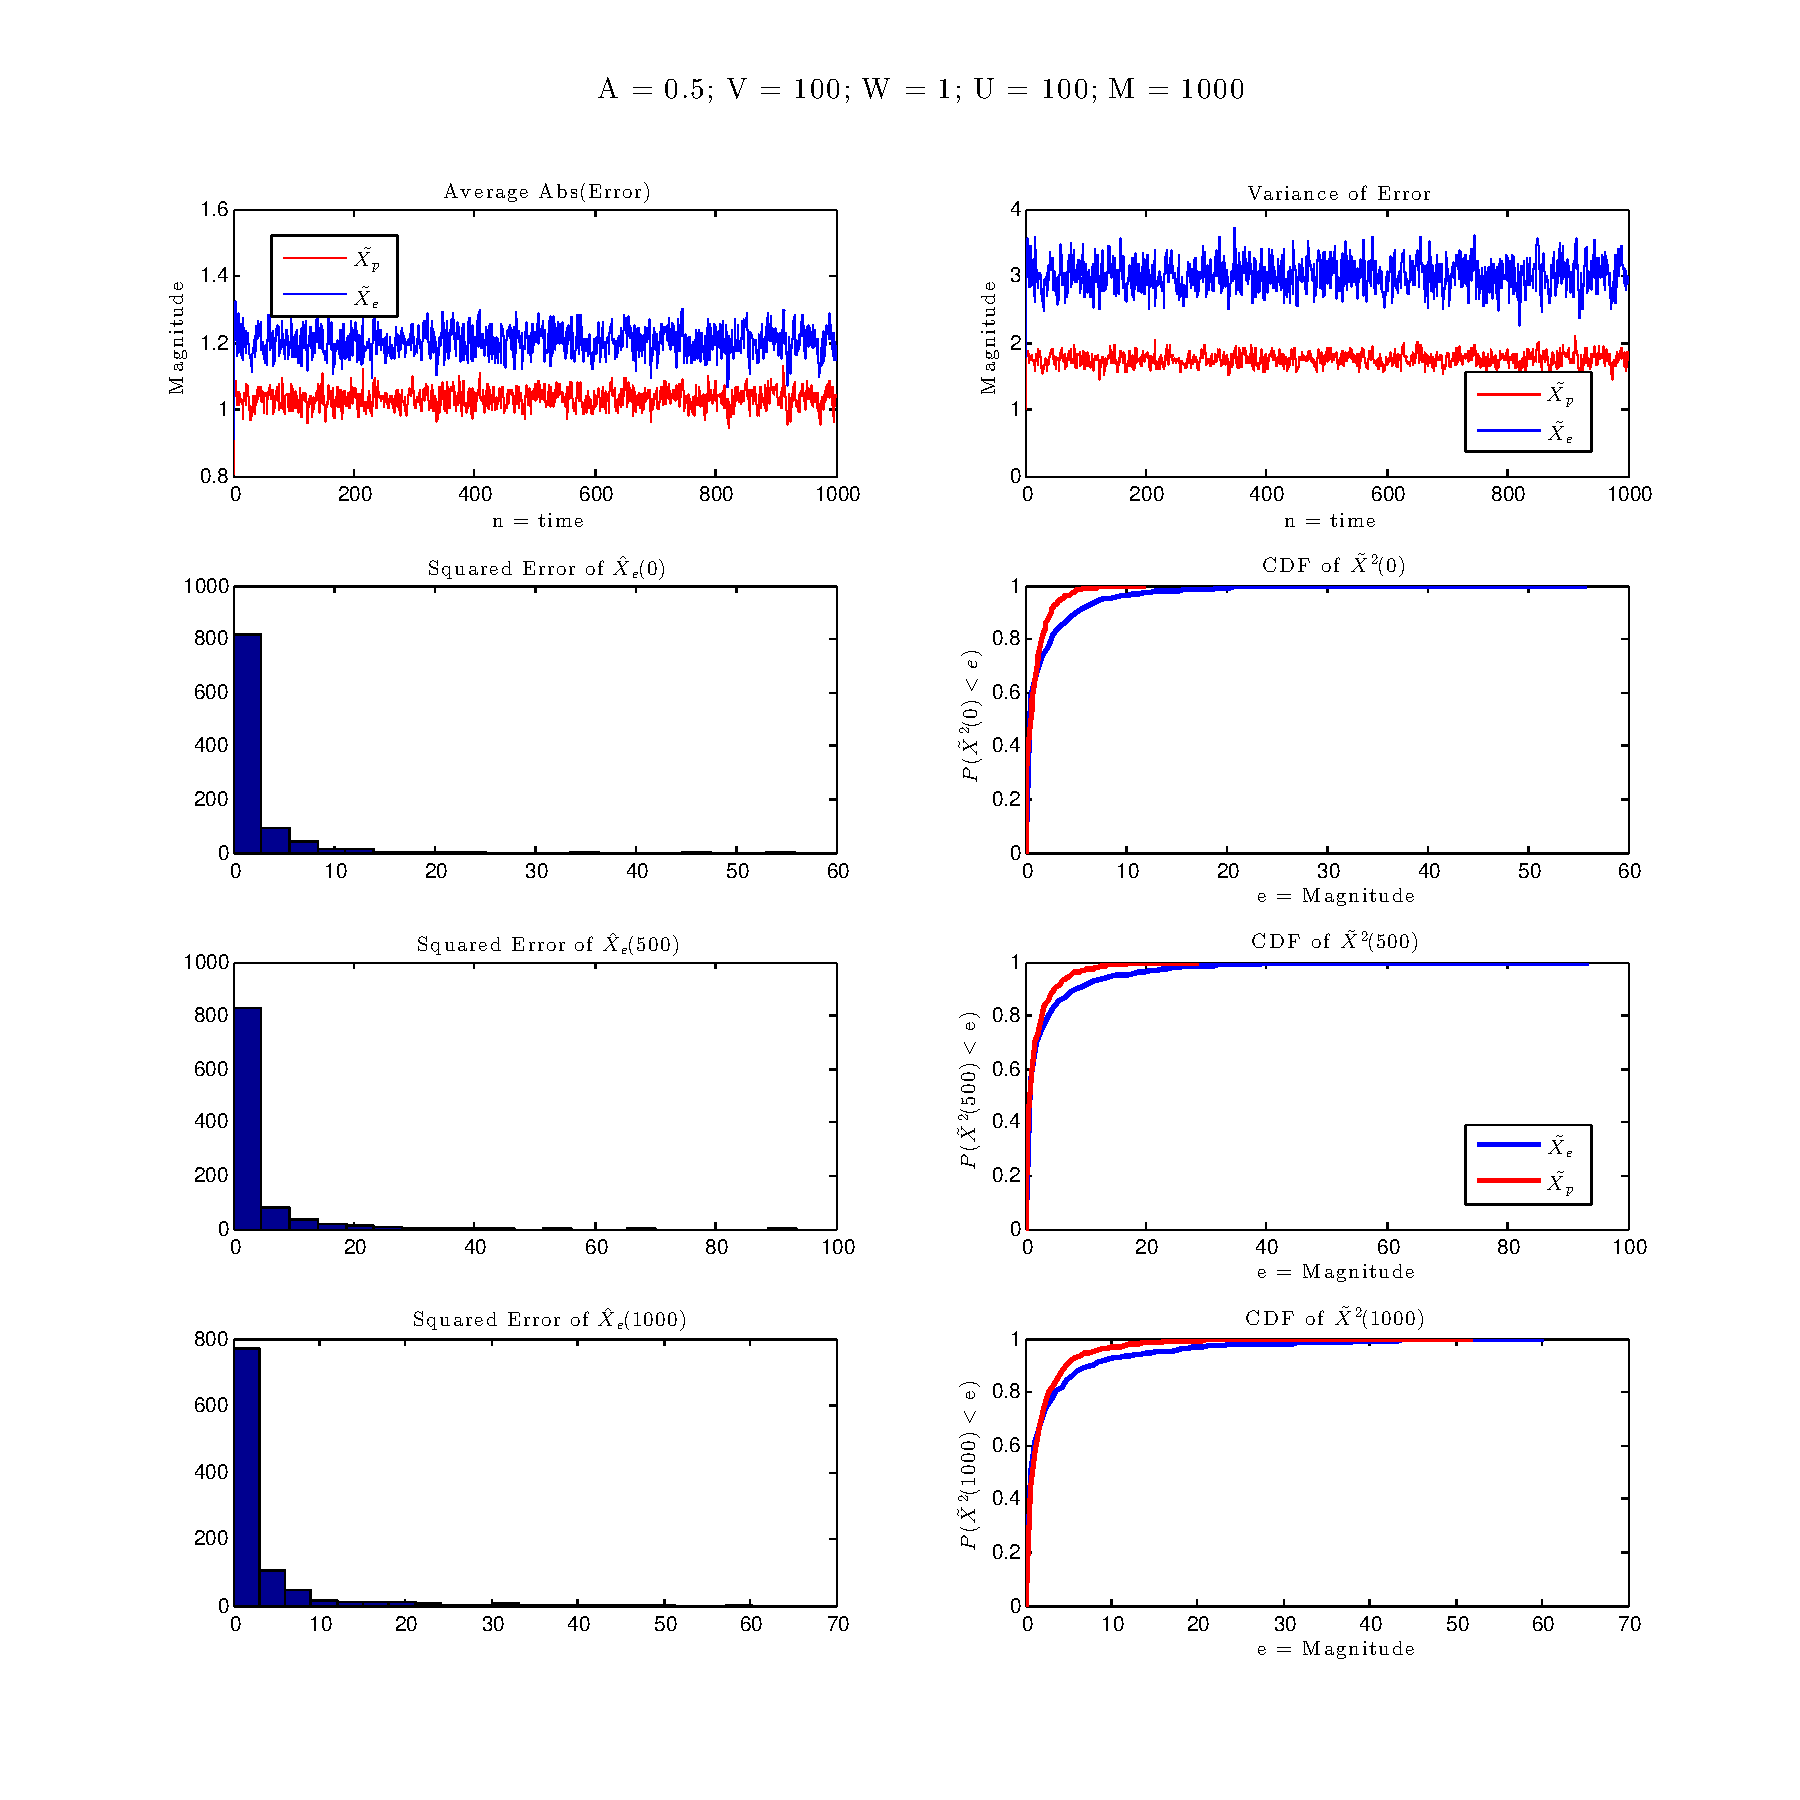
\includegraphics[width=\textwidth]{/Users/leahdickstein/Dropbox/R.edu/Sahai/140710/raj_a05_p001}
\end{minipage}
\begin{minipage}[c]{0.5\textwidth}
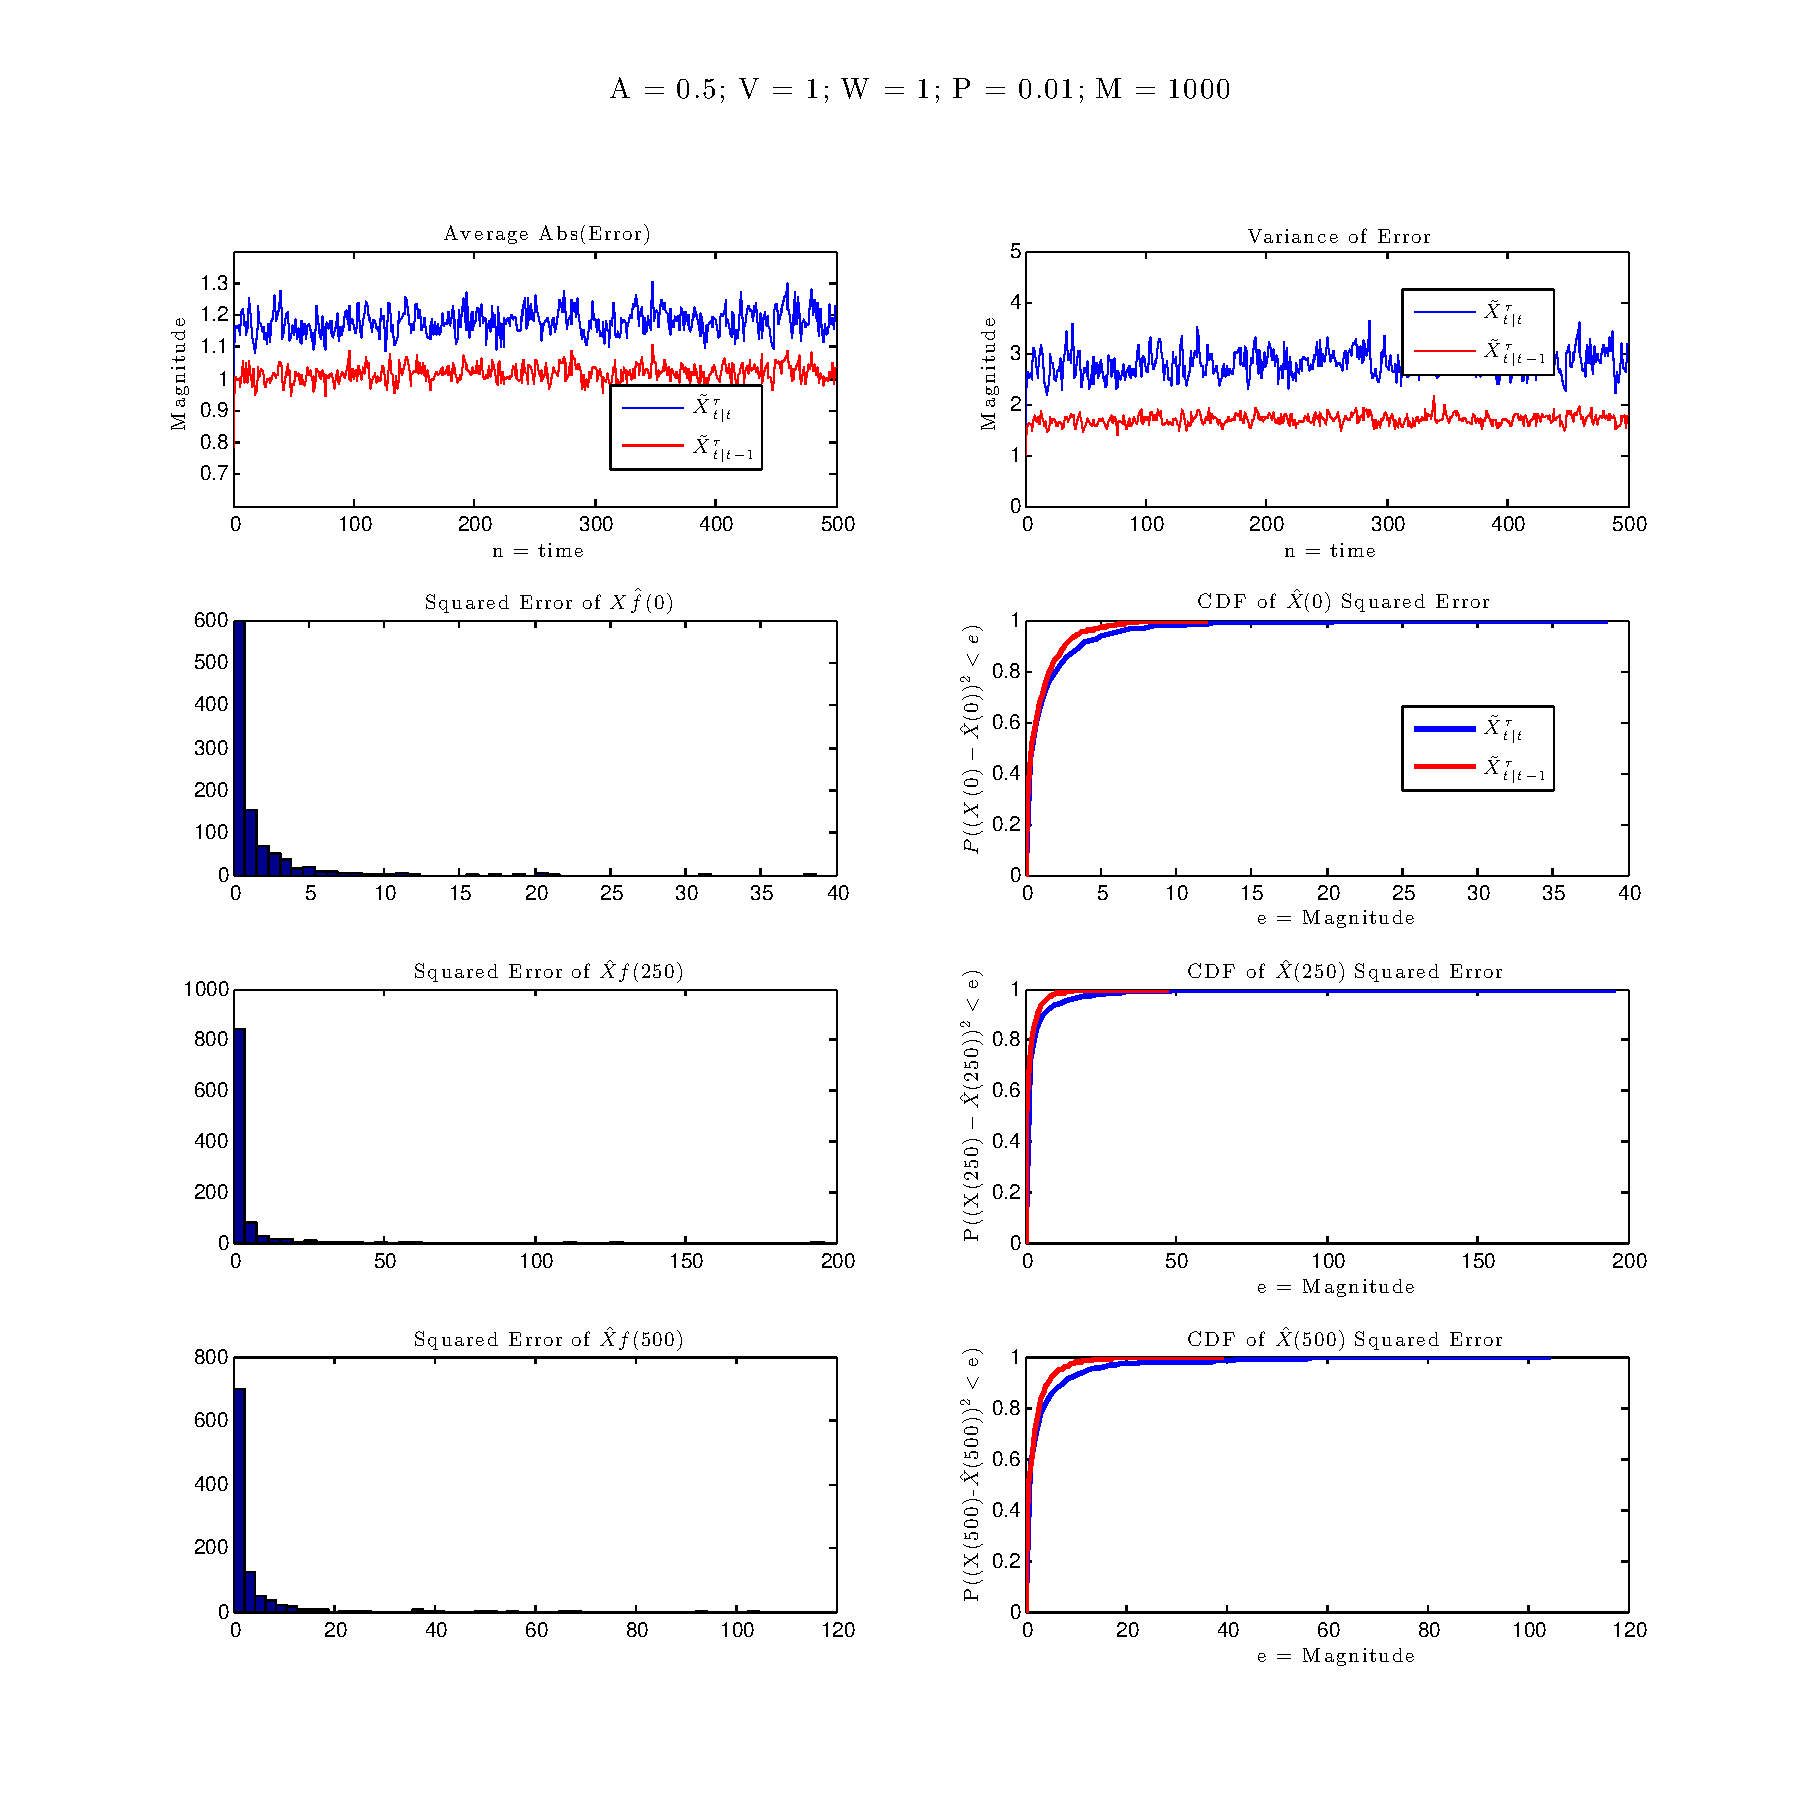
\includegraphics[width=\textwidth]{/Users/leahdickstein/Dropbox/R.edu/Sahai/140710/schenato_a05_p001}
\end{minipage}

Left = Rajasekaran's Kalman Filter, Right = Schenato's Receiver Estimators.\\
In all four figures, red represents prediction and blue represents estimation. 

\end{document}